%%%%%%%%%%%%%%%%%%%%%%%%%%%%%%%%%%%%%%%%%%%%%%%%%
%% Masters thesis presentation slides on
%% Training Neural Networks on Embedded Devices
%%
%% Uppsala Beamer theme
%% http://www.it.uu.se/katalog/daz/uppsala_beamer
%% by Frédéric Haziza <daz@it.uu.se>
%%%%%%%%%%%%%%%%%%%%%%%%%%%%%%%%%%%%%%%%%%%%%%%%%

\documentclass{beamer}
%\documentclass[handout]{beamer}
%\documentclass[notes]{beamer}
%\documentclass[trans]{beamer}

\usetheme[hideothersubsections]{Uppsala}

\usepackage{hyperref}
\usepackage{pgf}
\usepackage{tikz}
\usepackage{listofitems}

\usepgflibrary{arrows}
\usepgflibrary{shapes}

\usetikzlibrary{%
  arrows.meta,%
  calc,%
  fit,%
}

\usepackage[english]{babel} % or whatever
\usepackage[utf8]{inputenc} % or whatever

\usepackage{mathptmx}
\usepackage{helvet}

\usepackage[T1]{fontenc}

\title
{Training Neural Networks \\ on Embedded Devices}
\subtitle{Targeting Embedded Environments}

\author[Prasanth Shaji, Deepak Venkataram]
{Prasanth Shaji, Deepak Venkataram}

\institute[Dept. of Information Technology]
{
  Master's Thesis \\
  Uppsala University
}

\date[HDR-NN]
{\today}

%% \logo{...}

\subject{Uppsala University Master's Thesis on Training Neural Networks on Embedded Devices using the Beamer Theme for Uppsala University}

%% Unfolds piecewise element with shading.
%% Text appears, shaded, and the audience knows that somehting is coming
%% Note: if you set the number too high, the audience will try to read the
%% text that now shows up more, and will be disturbed.
%% ``dynamic'' makes elements show gradually more and more.
\setbeamercovered{transparent=9}
% \setbeamercovered{dynamic=5}

% ============================================
%        Presentation
% ============================================

\begin{document}

\begin{frame}[plain]
  \titlepage
\end{frame}

\begin{frame}
    \frametitle{Outline}
    \tableofcontents
\end{frame}

\section{NN in Embedded Devices}

\begin{frame}
  \frametitle{Neural Network Applications \\ on Embedded Devices}

  \begin{figure}
    \centering
    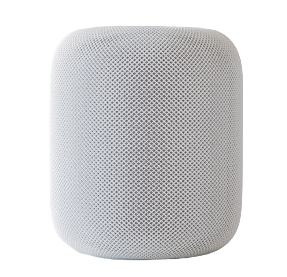
\includegraphics[scale=0.42]{images/smart-speaker}
    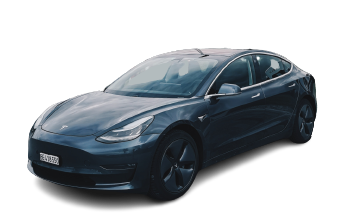
\includegraphics[scale=0.42]{images/tesla}
  \end{figure}

\end{frame}

\begin{frame}
  \frametitle{Embedded Devices}

  \begin{figure}
    \centering
    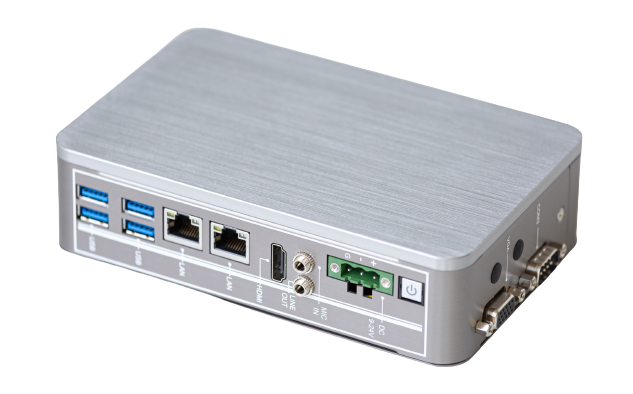
\includegraphics[scale=0.21]{images/edge-pc}
    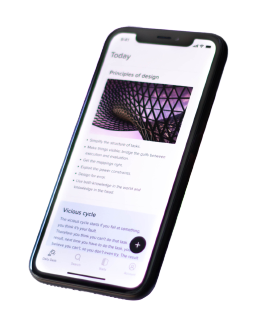
\includegraphics[scale=0.17]{images/smart-phone}
    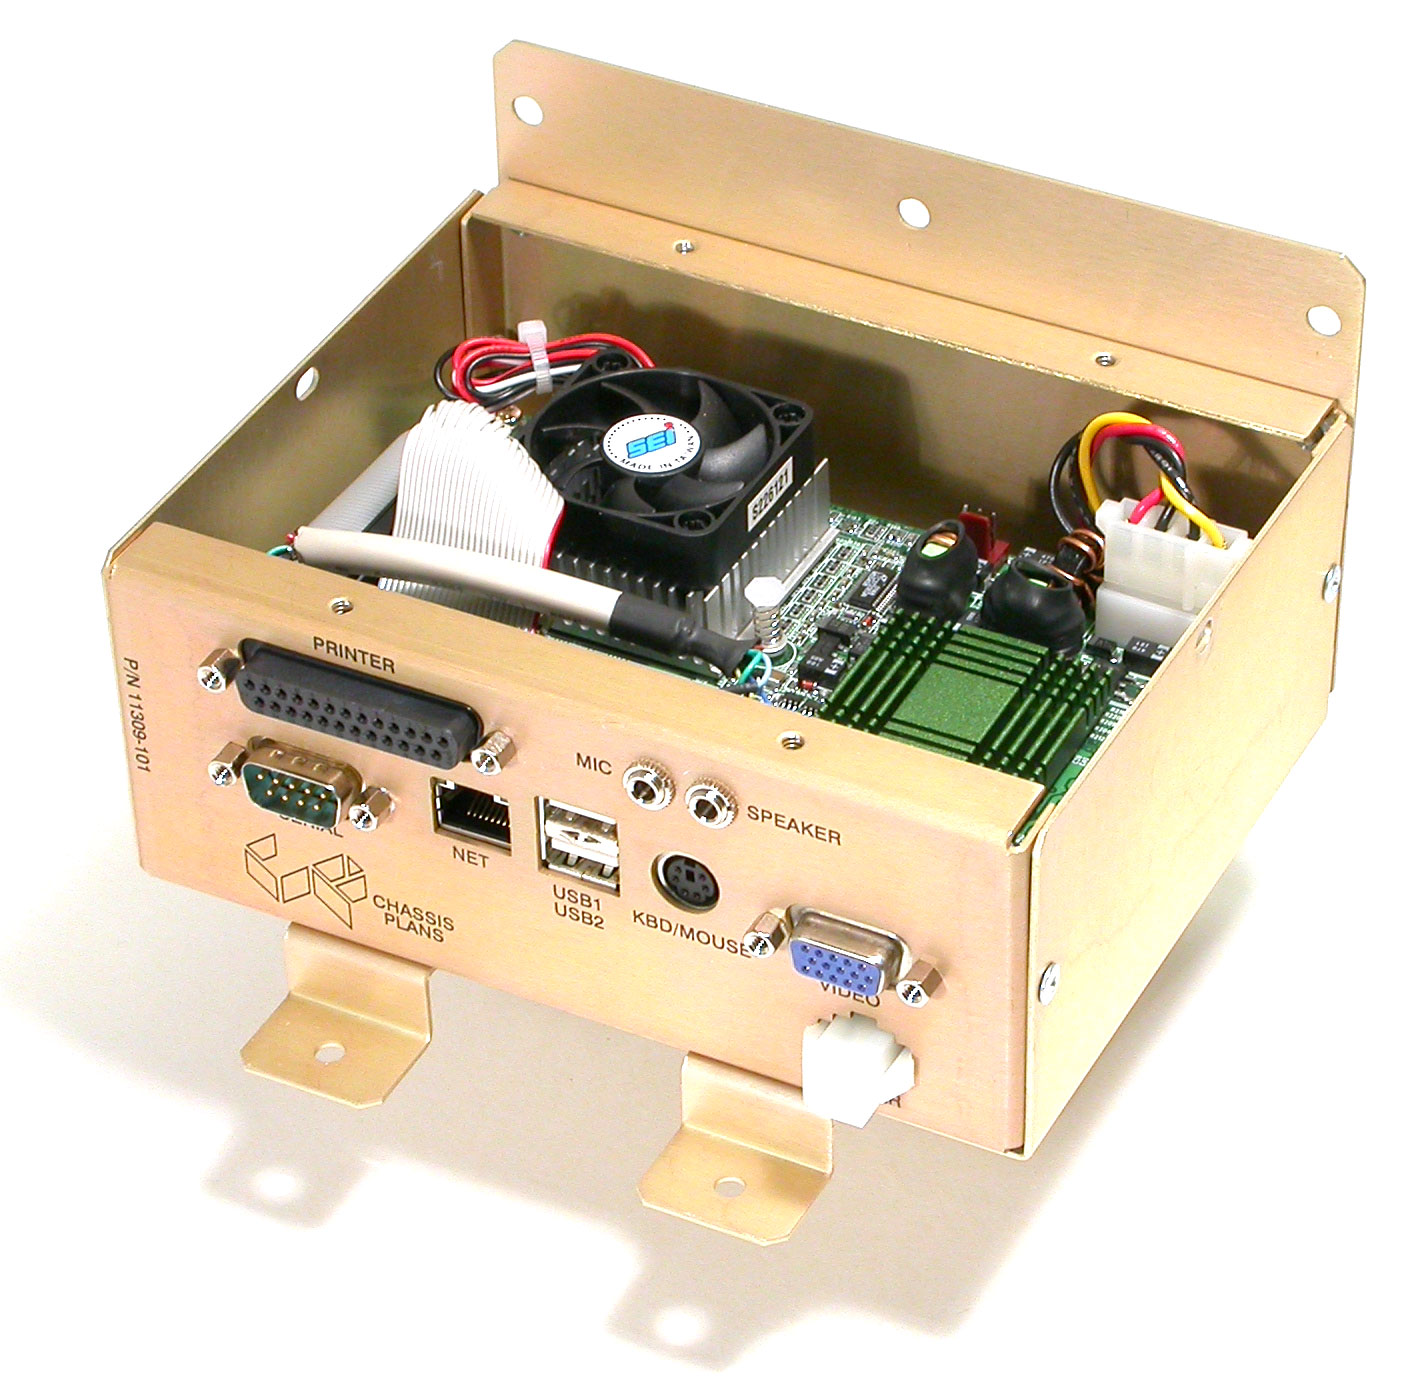
\includegraphics[scale=0.07]{images/accupoll-embedded-computer}\hspace{2em}
    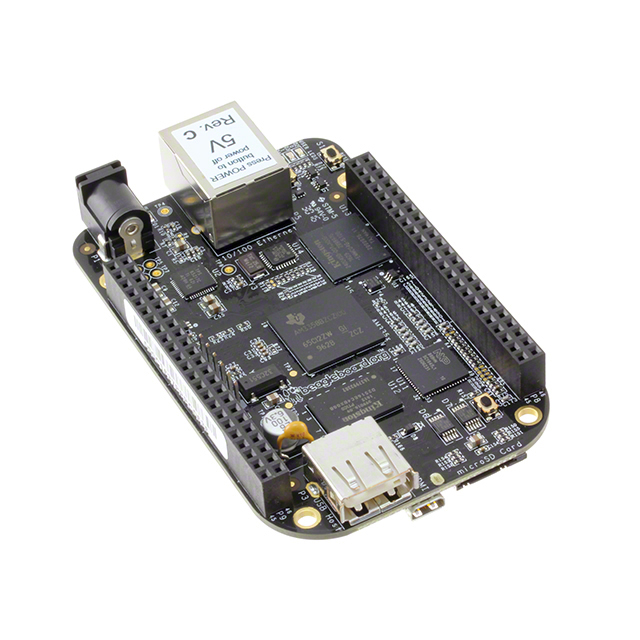
\includegraphics[scale=0.175]{../Body/images/bbb}
  \end{figure}

\end{frame}

\begin{frame}
  \frametitle{Goal : Neural Network training \\ on Scania C300}

  \begin{figure}
    \centering
    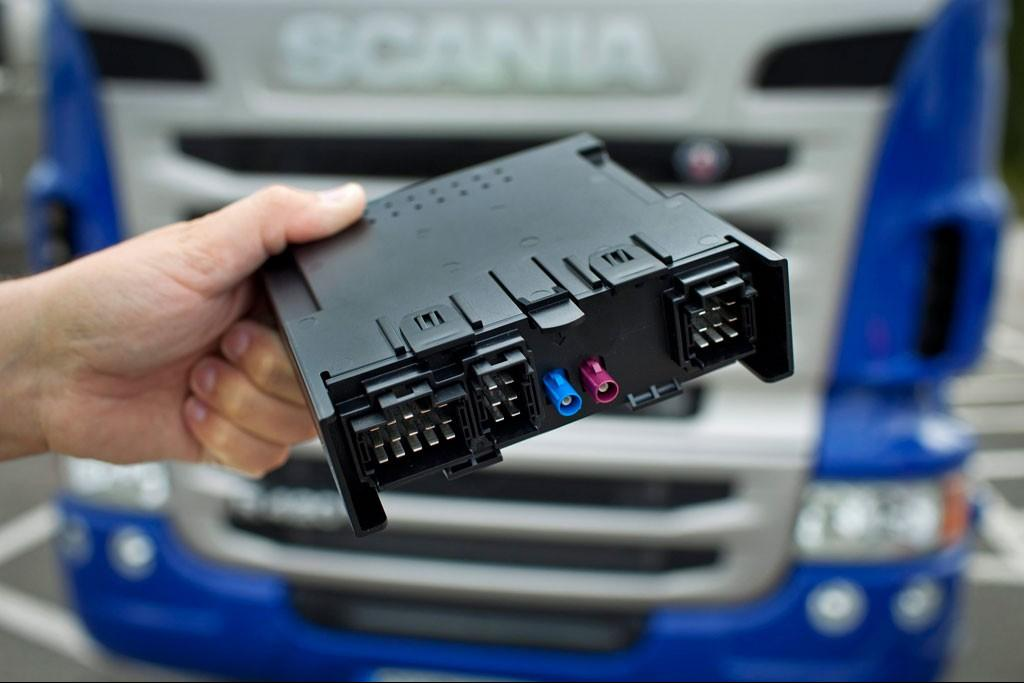
\includegraphics[scale=0.21]{../Body/images/c300.jpeg}
  \end{figure}

\end{frame}

\begin{frame}
  \frametitle{Goal : Neural Network training \\ on Scania C300}

  \onslide<1>
    Predictive vehicle maintenance using data from a fleet of connected trucks \\

  \onslide<2>
    Why Training on the C300?
    \begin{itemize}
  \onslide<2>
        \item Repurpose existing C300 units to perform neural network related tasks
        \item Training on devices to reduce network bandwidth usage, ensure data privacy, etc.
    \end{itemize}

    \vskip 1cm
  \onslide<3>
    \textbf{Scope} \textit{Repurpose Scania C300, train neural network model, assess training performance}

\end{frame}

\begin{frame}
  \frametitle{ARM Boards}

  \begin{table}[h]
    \centering
    \resizebox{\columnwidth}{!}{%
    \begin{tabular}{ |p{5em}|p{10em}|p{7em}|p{10em}| }
      \hline
        \textbf{SoC} &
        \textbf{Application Domain} &
        \textbf{Architecture} &
        \textbf{Processor Core} \\
      \hline
        nRF51822 &
        Ultra low power, BLE &
        ARM v6-M &
        ARM Cortex M0 \\
      \hline
        AM2732 &
        Automotive &
        ARM v7-R &
        ARM Cortex R5 \\
      \hline
        AM3358 &
        Industrial / IoT &
        ARM v7-A &
        ARM Cortex A8 \\
      \hline
        i.MX6S &
        Multimedia applications &
        ARM v7-A &
        ARM Cortex A9 \\
      \hline
        Kryo 240 &
        Smartphones &
        ARM v8-A &
        ARM Cortex-A73, A53 \\
      \hline
    \end{tabular}%
    }
  \end{table}
\end{frame}

\begin{frame}
  \frametitle{ARM Boards}

  \begin{figure}[h]
    \centering
    \resizebox{\columnwidth}{!}{%
    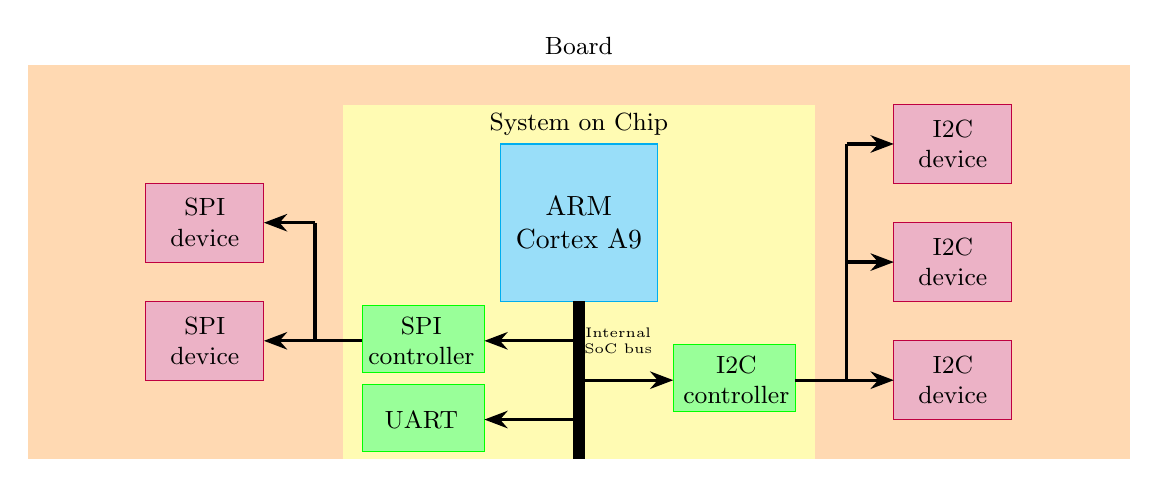
\begin{tikzpicture}[font=\small, >=Stealth]

      \fill [fill=orange!30] (0, 0) rectangle (14, 5);
      \draw (7, 5.25) node {Board};

      \fill [fill=yellow!30] (4, 0) rectangle (10, 4.5);
      \draw (7, 4.25) node {System on Chip};

      \draw [fill=cyan!40, draw=cyan] (6, 2) rectangle (8, 4);
      \draw (7, 3) node[align=center, font=\normalsize]
        {ARM \\ Cortex A9};

      \draw [line width=0.42em] (7, 2) -- (7, 0);
      \draw (7.5, 1.5) node[align=center, font=\tiny]
        {Internal \\ SoC bus};

      \draw [fill=green!40, draw=green] (4.25, 1.1) rectangle (5.8, 1.95);
      \draw (5, 1.5) node[align=center] {SPI \\ controller};
      \draw [<-, very thick] (5.8, 1.5) -- (7, 1.5);

      \draw [fill=green!40, draw=green] (4.25, 0.1) rectangle (5.8, 0.95);
      \draw (5, 0.5) node {UART};
      \draw [<-, very thick] (5.8, 0.5) -- (7, 0.5);

      \draw [fill=purple!30, draw=purple] (1.5, 1) rectangle (3, 2);
      \draw (2.25, 1.5) node[align=center] {SPI \\ device};
      \draw [<-, very thick] (3, 1.5) -- (4.25, 1.5);

      \draw [very thick] (3.65, 1.5) -- (3.65, 3);

      \draw [fill=purple!30, draw=purple] (1.5, 2.5) rectangle (3, 3.5);
      \draw (2.25, 3) node[align=center] {SPI \\ device};
      \draw [<-, very thick] (3, 3) -- (3.65, 3);

      \draw [fill=green!40, draw=green] (8.2, 0.6) rectangle (9.75, 1.45);
      \draw (9, 1) node[align=center] {I2C \\ controller};
      \draw [->, very thick] (7, 1) -- (8.2, 1);

      \draw [very thick] (10.4, 1) -- (10.4, 4);

      \draw [fill=purple!30, draw=purple] (11, 0.5) rectangle (12.5, 1.5);
      \draw (11.75, 1) node[align=center] {I2C \\ device};
      \draw [->, very thick] (9.75, 1) -- (11, 1);

      \draw [fill=purple!30, draw=purple] (11, 2) rectangle (12.5, 3);
      \draw (11.75, 2.5) node[align=center] {I2C \\ device};
      \draw [->, very thick] (10.4, 2.5) -- (11, 2.5);

      \draw [fill=purple!30, draw=purple] (11, 3.5) rectangle (12.5, 4.5);
      \draw (11.75, 4) node[align=center] {I2C \\ device};
      \draw [->, very thick] (10.4, 4) -- (11, 4);

    \end{tikzpicture}%
    }
  \end{figure}

\end{frame}

\section{Embedded Linux}

\begin{frame}
  \frametitle{Embedded Linux}

  Operating System for Embedded Devices \\
  - Customized for Specific Hardware

  \vspace{4em}
  Kernel, Bootloaders, Device Trees \\
  Cross Compilation, Toolchains, Root Filesystems

\end{frame}

\begin{frame}
  \frametitle{Software Versions}

  \begin{figure}
    \centering
    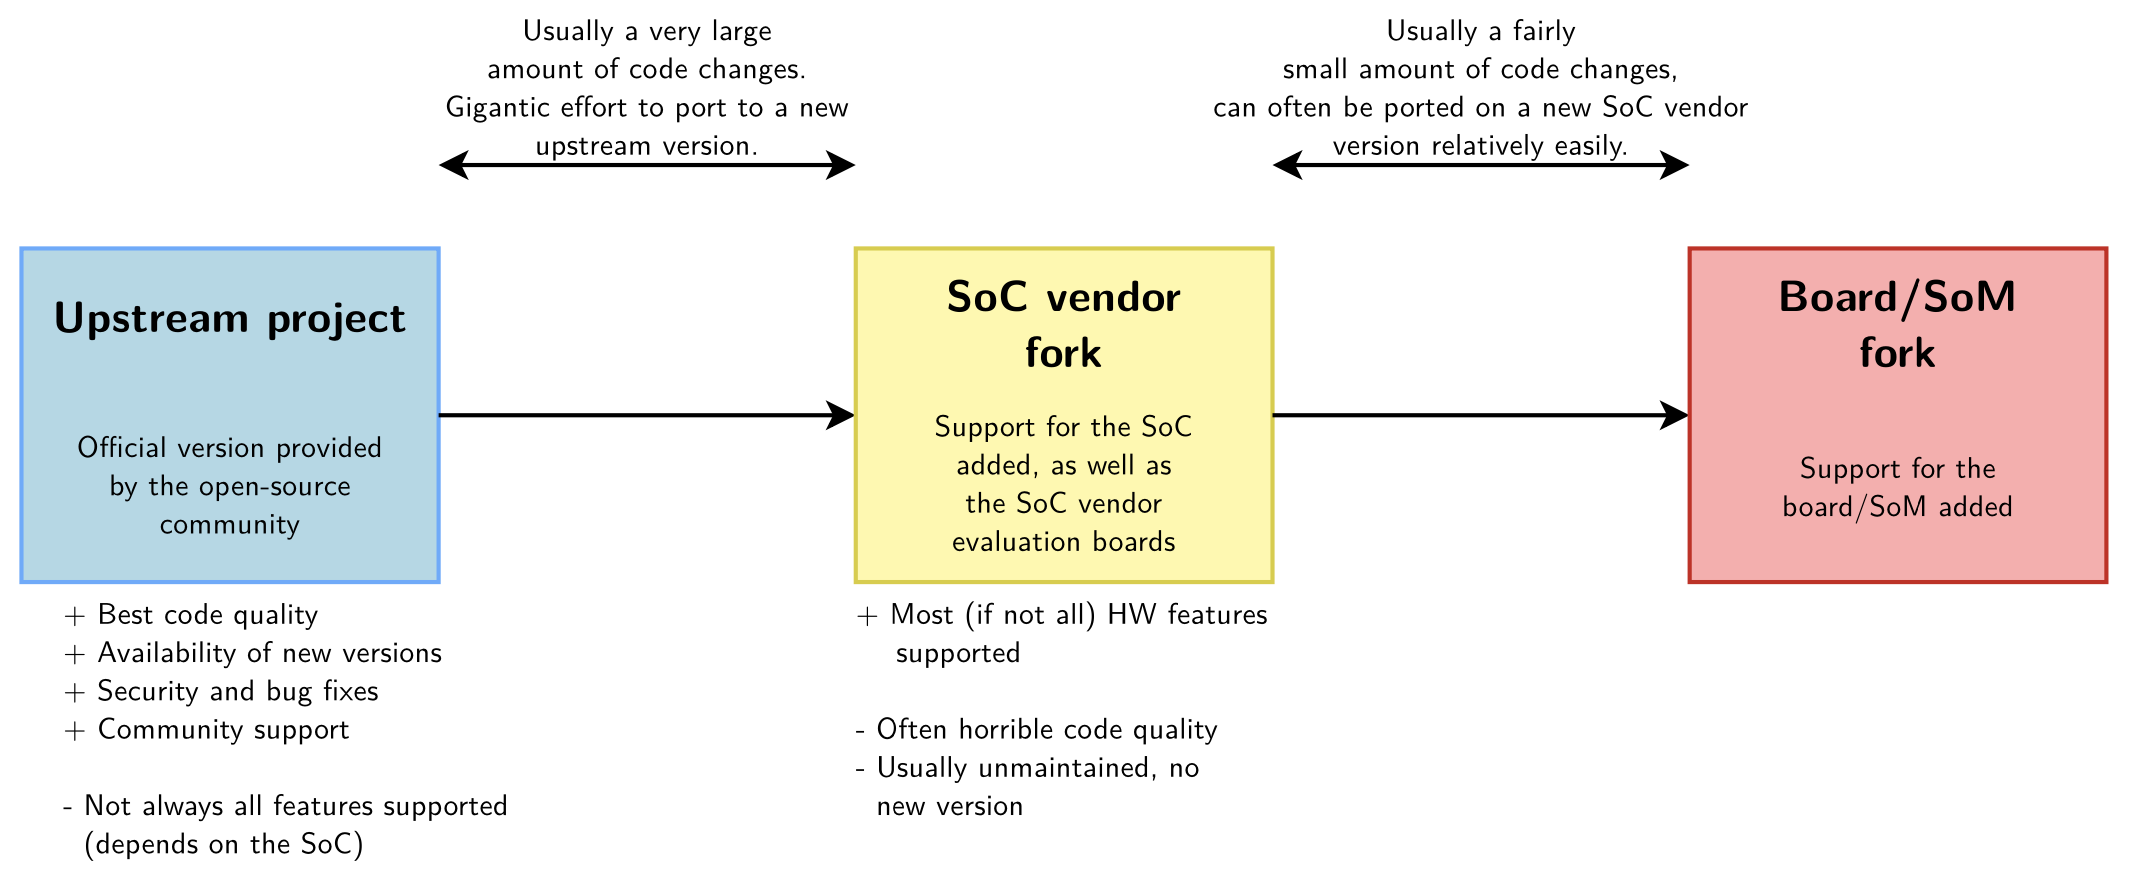
\includegraphics[scale=0.27]{images/sw-versions.png}
  \end{figure}

\end{frame}

\begin{frame}
  \frametitle{Build Systems}

  Yocto Project

  \begin{figure}
    \centering
    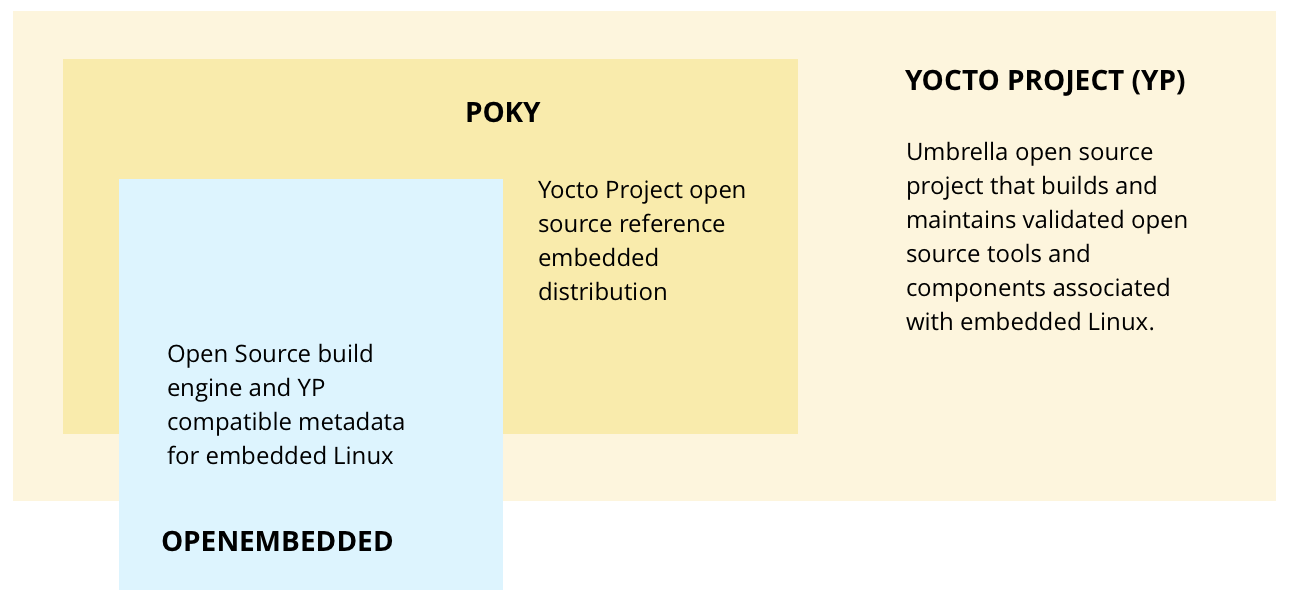
\includegraphics[scale=0.42]{images/yp-diagram-overview.png}
  \end{figure}

\end{frame}

\begin{frame}
  \frametitle{Yocto Project}

  \begin{figure}
    \centering
    \scalebox{0.52}{
    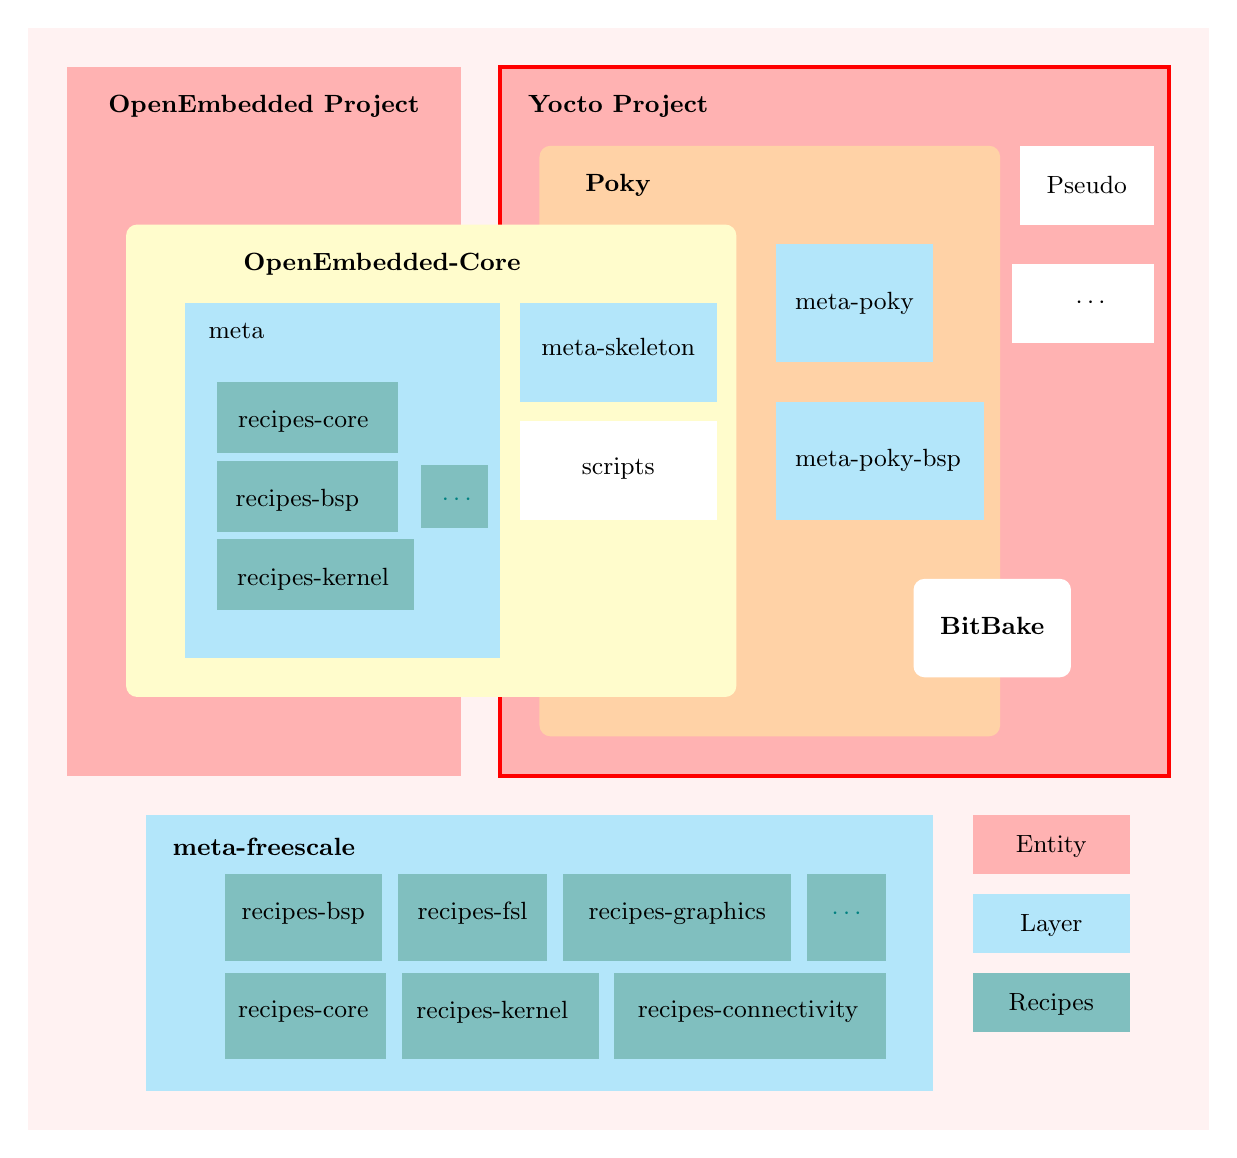
\begin{tikzpicture}[font=\small]

      \fill [fill=pink!20] (-0.5, -4.5) rectangle (14.5, 9.5);

      \fill [fill=red!30] (0, 0) rectangle (5, 9);
      \draw (2.5, 8.5) node {\textbf{OpenEmbedded Project}};

      \draw [fill=red!30, draw=red, line width=1.4pt] (5.5, 0) rectangle (14, 9);
      \draw (7, 8.5) node {\textbf{Yocto Project}};

      \fill [orange!35, rounded corners] (6, 0.5) rectangle (11.85, 8);
      \draw (7, 7.5) node {\textbf{Poky}};

      \fill [yellow!20, rounded corners] (0.75, 1) rectangle (8.5, 7);
      \draw (4, 6.5) node {\textbf{OpenEmbedded-Core}};

      \fill [cyan!30] (1.5, 1.5) rectangle (5.5, 6);
      \draw (2.15, 5.65) node {meta};

      \fill [teal!50] (1.9, 4.1) rectangle (4.2, 5);
      \draw (3, 4.5) node {recipes-core};

      \fill [teal!50] (1.9, 3.1) rectangle (4.2, 4);
      \draw (2.925, 3.5) node {recipes-bsp};

      \fill [teal!50] (1.9, 2.1) rectangle (4.4, 3);
      \draw (3.125, 2.5) node {recipes-kernel};

      \fill [teal!50] (4.5, 3.15) rectangle (5.35, 3.95);
      \draw (4.95, 3.5) node[text=teal] {\textbf{$\cdots$}};

      \fill [cyan!30] (5.75, 4.75) rectangle (8.25, 6);
      \draw (7, 5.45) node {meta-skeleton};

      \fill [white!40] (5.75, 3.25) rectangle (8.25, 4.5);
      \draw (7, 3.9) node {scripts};

      \fill [cyan!30] (9, 5.25) rectangle (11, 6.75);
      \draw (10, 6) node {meta-poky};

      \fill [cyan!30] (9, 3.25) rectangle (11.65, 4.75);
      \draw (10.3, 4) node {meta-poky-bsp};

      \fill [white!40, rounded corners] (10.75, 1.25) rectangle (12.75, 2.5);
      \draw (11.75, 1.9) node {\textbf{BitBake}};

      \fill [white!40] (12.1, 7) rectangle (13.8, 8);
      \draw (12.95, 7.5) node {Pseudo};

      \fill [white!40] (12, 5.5) rectangle (13.8, 6.5);
      \draw (13, 6) node {\textbf{$\cdots$}};

      \fill [cyan!30] (1, -4) rectangle (11, -0.5);
      \draw (2.5, -0.9) node {\textbf{meta-freescale}};

      \fill [teal!50] (2, -2.35) rectangle (4, -1.25);
      \draw (3, -1.75) node {recipes-bsp};

      \fill [teal!50] (4.2, -2.35) rectangle (6.1, -1.25);
      \draw (5.15, -1.75) node {recipes-fsl};

      \fill [teal!50] (6.3, -2.35) rectangle (9.2, -1.25);
      \draw (7.75, -1.75) node {recipes-graphics};

      \fill [teal!50] (9.4, -2.35) rectangle (10.4, -1.25);
      \draw (9.9, -1.75) node[text=teal] {\textbf{$\cdots$}};

      \fill [teal!50] (2, -3.6) rectangle (4.05, -2.5);
      \draw (3, -3) node {recipes-core};

      \fill [teal!50] (4.25, -3.6) rectangle (6.75, -2.5);
      \draw (5.4, -3) node {recipes-kernel};

      \fill [teal!50] (6.95, -3.6) rectangle (10.4, -2.5);
      \draw (8.65, -3) node {recipes-connectivity};

      \fill [red!30] (11.5, -1.25) rectangle (13.5, -0.5);
      \draw (12.5, -0.9) node {Entity};

      \fill [cyan!30] (11.5, -2.25) rectangle (13.5, -1.5);
      \draw (12.5, -1.9) node {Layer};

      \fill [teal!50] (11.5, -3.25) rectangle (13.5, -2.5);
      \draw (12.5, -2.9) node {Recipes};
    \end{tikzpicture}}
  \end{figure}

\end{frame}

\begin{frame}
  \frametitle{Yocto Project}

  \begin{figure}
    \centering
    \scalebox{0.7}{
    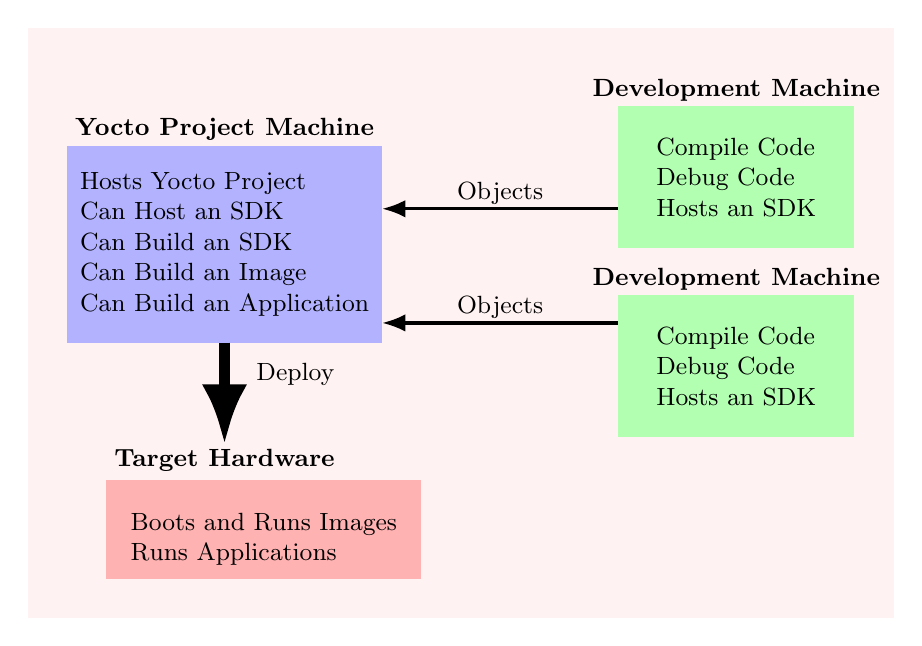
\begin{tikzpicture}[font=\small, >=Latex]

      \fill [fill=pink!20] (0, 0) rectangle (11, 7.5);

      \fill [fill=blue!30] (0.5, 3.5) rectangle (4.5, 6);
      \draw (2.5, 6.21) node {\textbf{Yocto Project Machine}};
      \draw (2.5, 4.75) node[align=left]
        {
          Hosts Yocto Project \\
          Can Host an SDK \\
          Can Build an SDK \\
          Can Build an Image \\
          Can Build an Application
        };

      \draw [<-, very thick] (4.5, 5.2) -- (7.5, 5.2);
      \draw (6, 5.4) node {Objects};

      \fill [fill=green!30] (7.5, 4.7) rectangle (10.5, 6.5);
      \draw (9, 6.7) node {\textbf{Development Machine}};
      \draw (9, 5.6) node[align=left]
        {
          Compile Code \\
          Debug Code \\
          Hosts an SDK
        };

      \draw [<-, very thick] (4.5, 3.75) -- (7.5, 3.75);
      \draw (6, 3.95) node {Objects};

      \fill [fill=green!30] (7.5, 2.3) rectangle (10.5, 4.1);
      \draw (9, 4.3) node {\textbf{Development Machine}};
      \draw (9, 3.2) node[align=left]
        {
          Compile Code \\
          Debug Code \\
          Hosts an SDK
        };

      \draw [->, line width=0.42em] (2.5, 3.5) -- (2.5, 2.2);
      \draw (3.4, 3.1) node {Deploy};

      \fill [fill=red!30] (1, 0.5) rectangle (5, 1.75);
      \draw (2.5, 2) node {\textbf{Target Hardware}};
      \draw (3, 1) node[align=left]
      {
        Boots and Runs Images \\
        Runs Applications
      };

    \end{tikzpicture}}
  \end{figure}

\end{frame}

\begin{frame}
  \frametitle{Scania C300 to MCIMX6Q-SDB}

  \begin{figure}
    \centering
    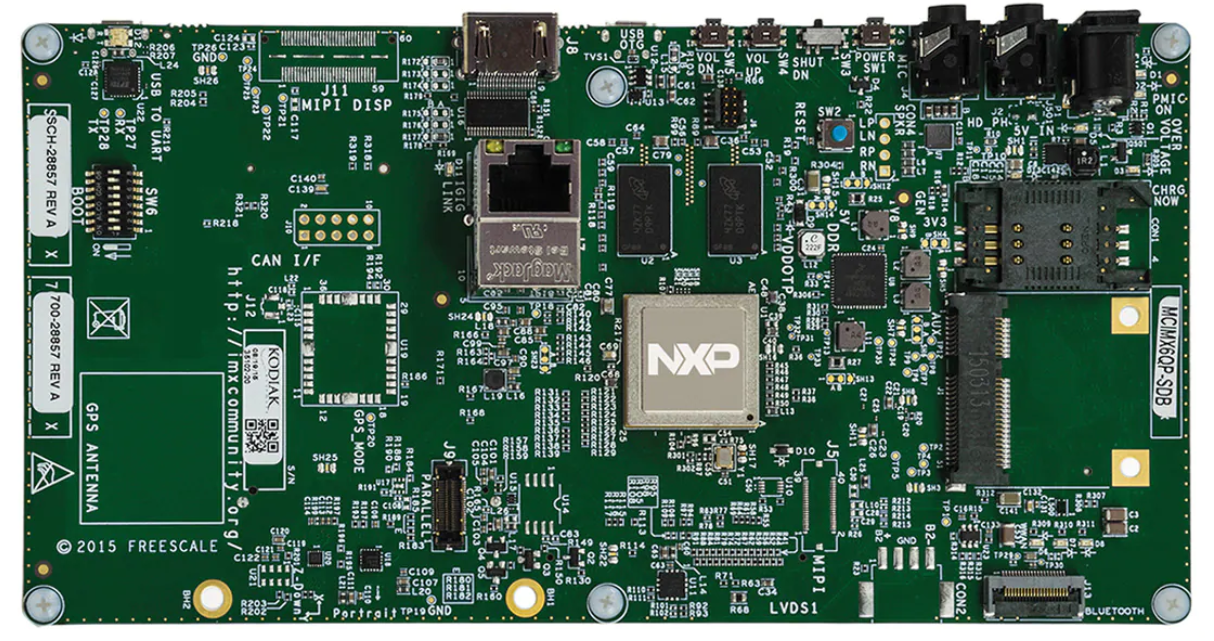
\includegraphics[scale=0.21]{../Body/images/MCIMX6Q-SDB-BD.png}
  \end{figure}

\end{frame}

\section{Neural Networks}

\begin{frame}
  \frametitle{Training and Inference}

  \begin{figure}
    \centering
    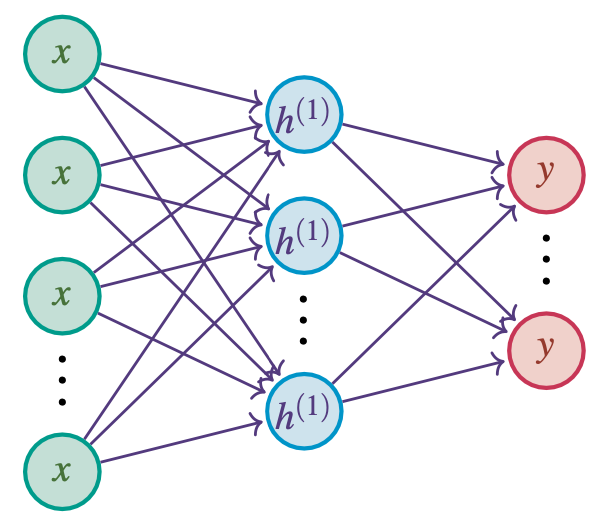
\includegraphics[scale=0.42]{images/network.png}
  \end{figure}

\end{frame}

\begin{frame}
  \frametitle{Traditional Paradigm}

  \begin{figure}
    \centering
    \begin{tikzpicture}

      \node (ecu) at (0,0) {
\includegraphics[scale=2]{../Body/images/truck.png}};

      \node (cloud) at (3.5, 2) {
\includegraphics[scale=2]{../Body/images/db.png}};

      \node (server) at (7, 0) {
\includegraphics[scale=2]{../Body/images/server.png}};
      \draw[-{Latex}, very thick, orange!90] ([xshift=14pt]server.north east) arc (355:0:0.25);

      \draw[->,thick] (ecu) -- (cloud);
      \draw[->,thick] (cloud) -- (server);
      \draw[->,thick] (server) -- (ecu);

    \end{tikzpicture}
  \end{figure}
\end{frame}

\begin{frame}
  \frametitle{Federated Learning}

  \begin{figure}
    \centering
    \begin{tikzpicture}[rounded corners, opacity=0.87]

      \readlist\Trucks {1,2,3,4}
      \foreachitem \x \in \Trucks
      {
        \node (ecu \x) at ({0 + 2.5 * (\x-1)}, 0) {
\includegraphics[scale=2]{../Body/images/truck.png}};
      }

      \node[inner xsep=21pt] (server) at (3.5, 2) {
\includegraphics[scale=1.8]{../Body/images/server.png}};
      \draw[-{Latex}, very thick, orange!90] ([yshift=-7pt]server.north east) arc (355:0:0.25);

      \foreachitem \x \in \Trucks
      {
        \draw[<->,thick] (ecu \x.north) -- (server);
        \draw[-{Latex}, very thick, orange!50] ([yshift=-7pt]ecu \x.north east) arc (355:0:0.25);
      }

    \end{tikzpicture}
  \end{figure}
\end{frame}

\section{Benchmark Applications}

\begin{frame}
  \frametitle{Handwritten Digit Recognition \\ Neural Network}

  \begin{figure}
    \centering
    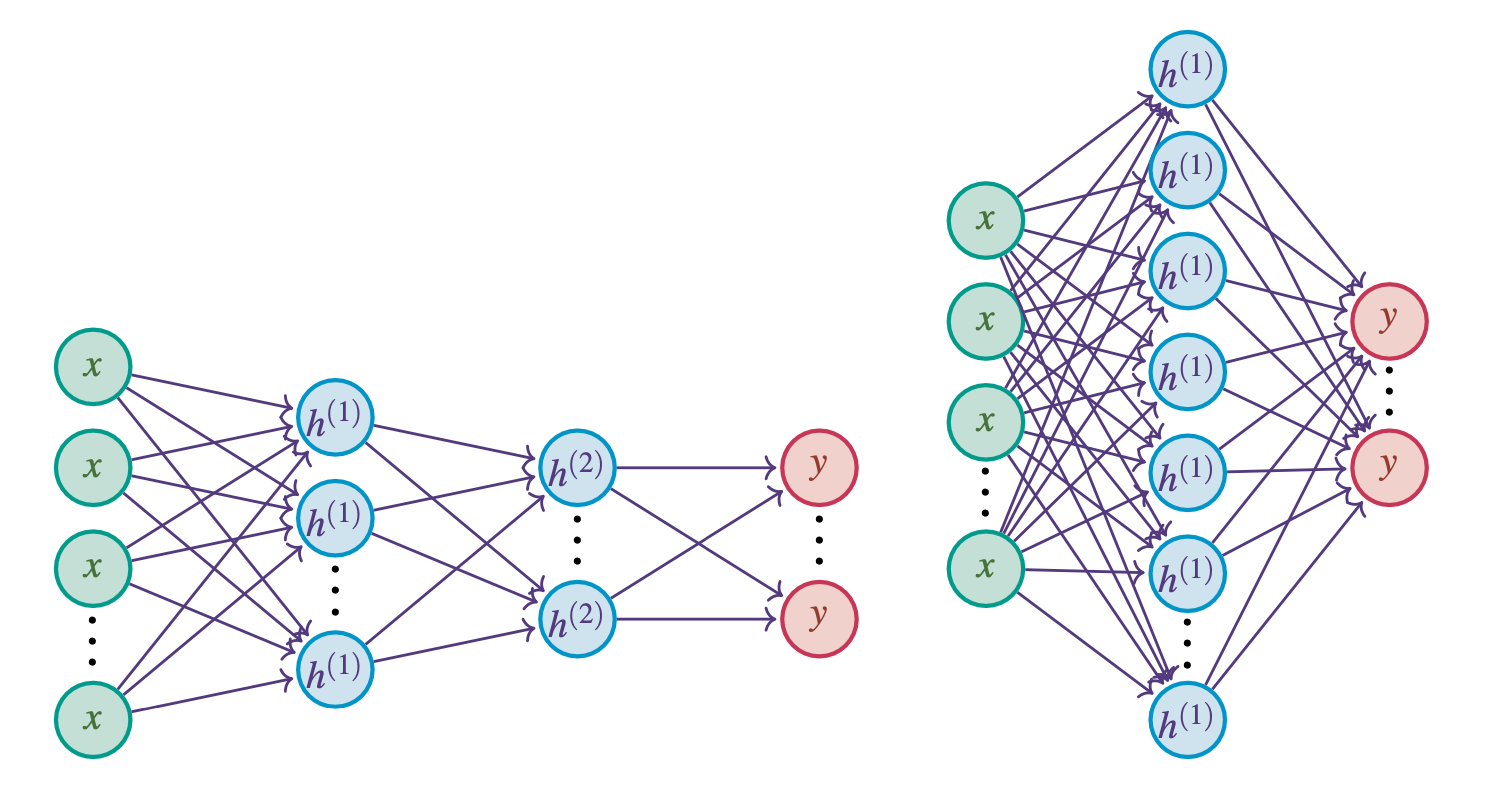
\includegraphics[scale=0.37]{images/networks.png}
  \end{figure}

\end{frame}

\begin{frame}
  \frametitle{Learning Algorithm}

  \begin{figure}
    \centering
    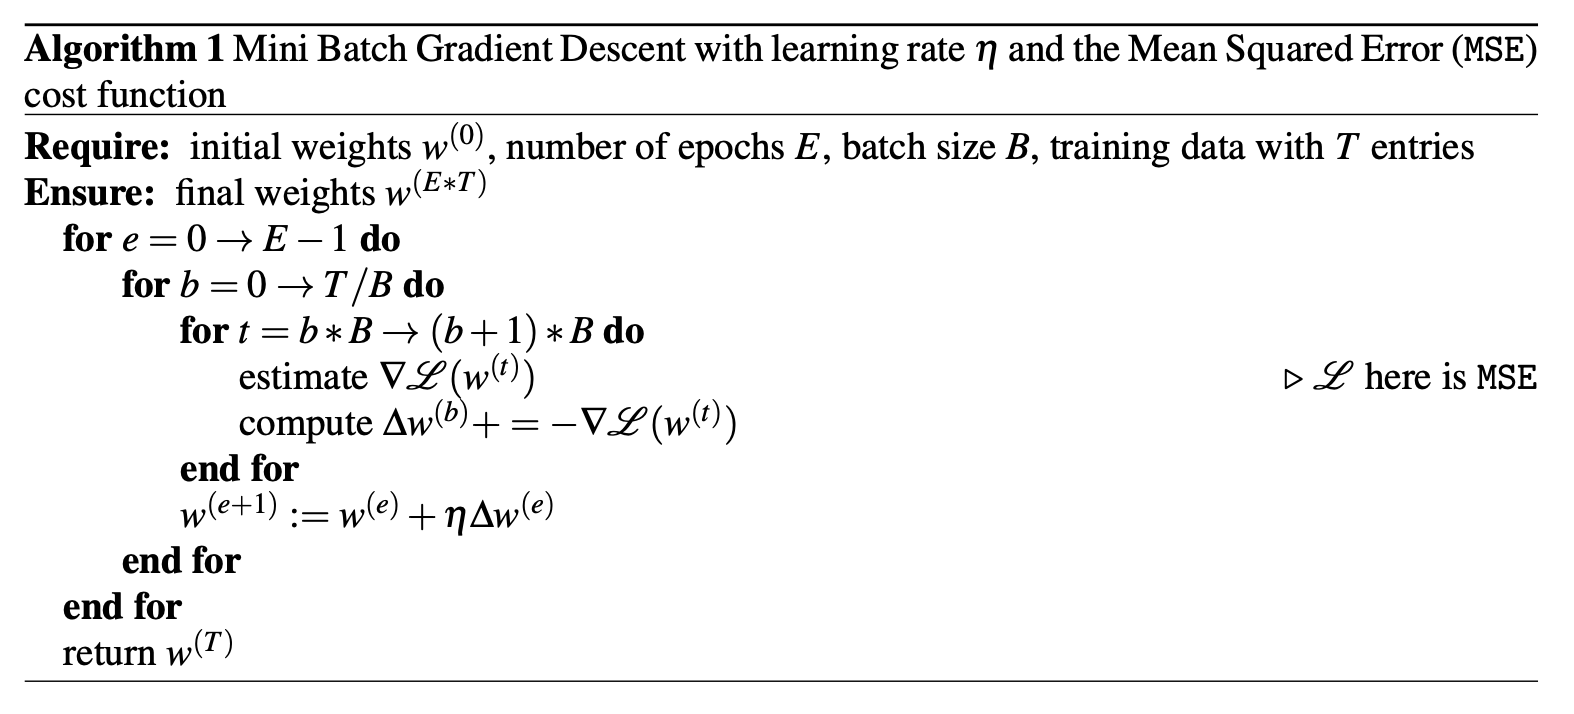
\includegraphics[scale=0.37]{images/mSGD.png}
  \end{figure}

\end{frame}

\begin{frame}
  \frametitle{HDR-NN configurability}

  \begin{figure}
    \centering
    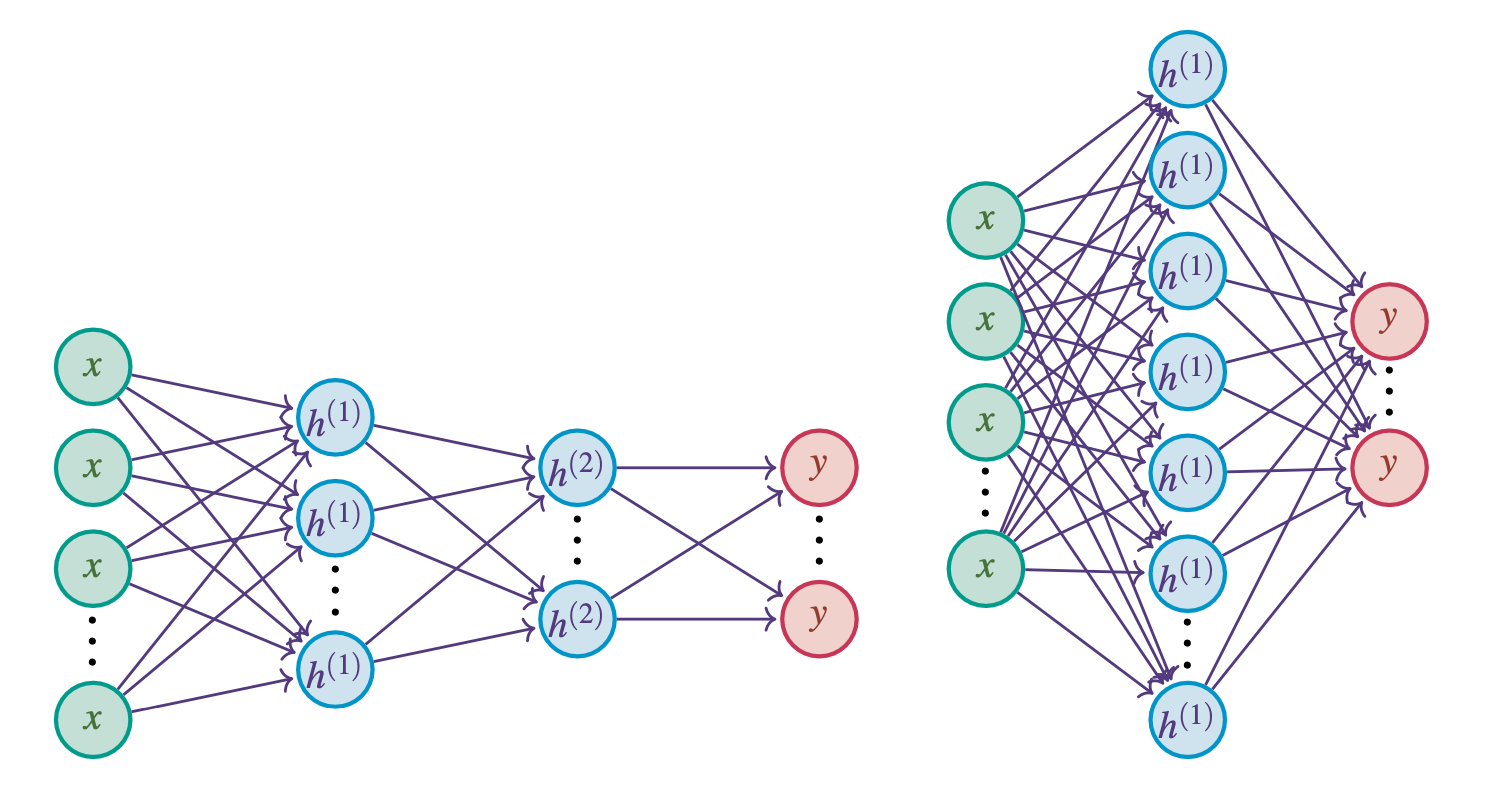
\includegraphics[scale=0.37]{images/networks.png}
  \end{figure}

\end{frame}

\begin{frame}
  \frametitle{HDR-NN configurability}

  \begin{figure}
    \centering
    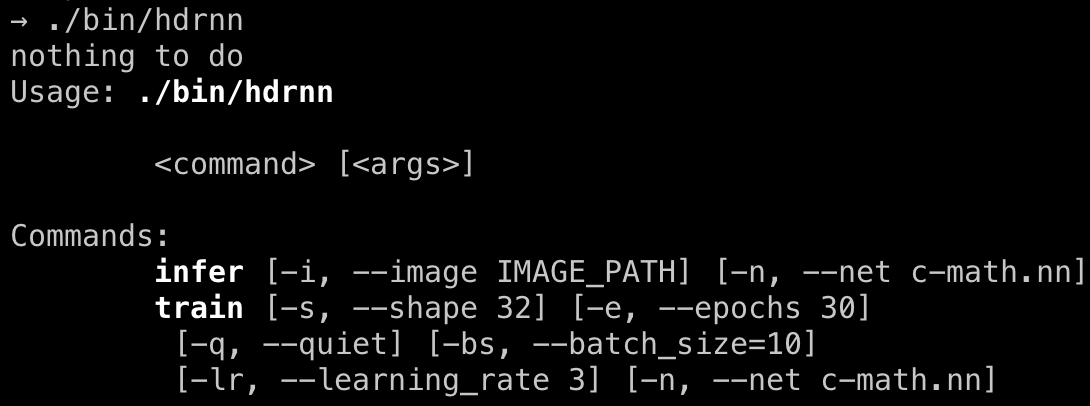
\includegraphics[scale=0.37]{images/usage.png}
  \end{figure}

\end{frame}

\begin{frame}
  \frametitle{C based HDR-NN}

  \begin{figure}
    \centering
    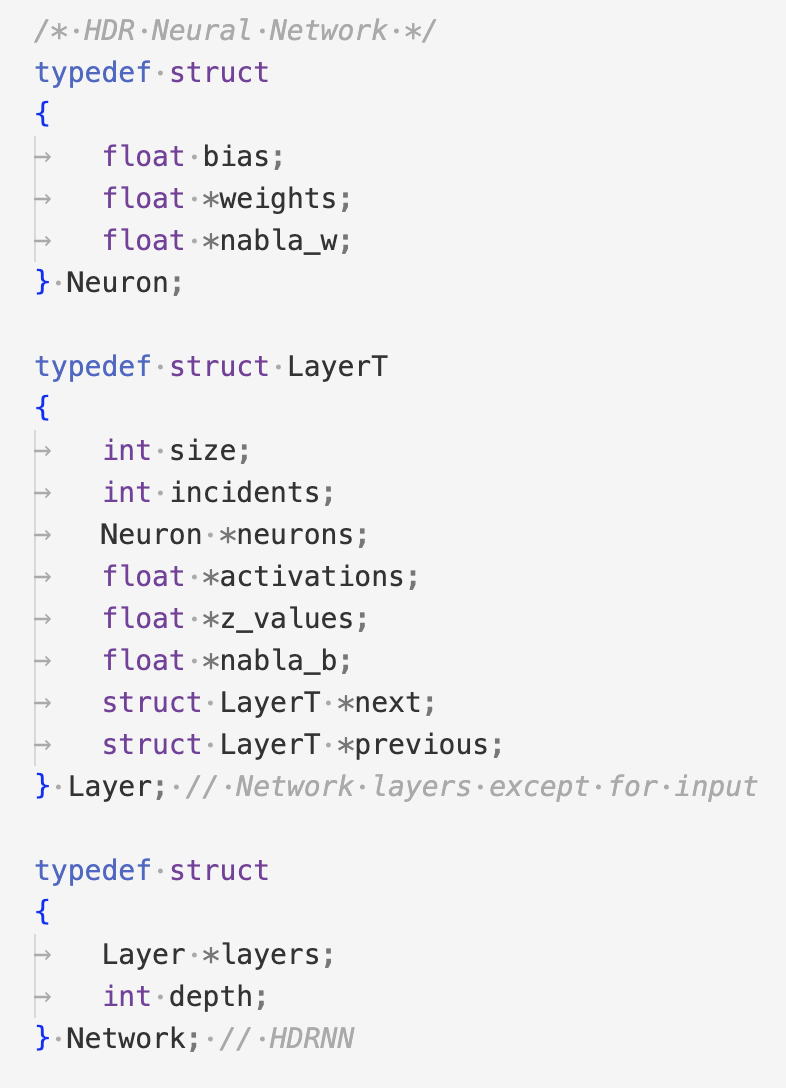
\includegraphics[scale=0.30]{images/c-hdrnn.png}
    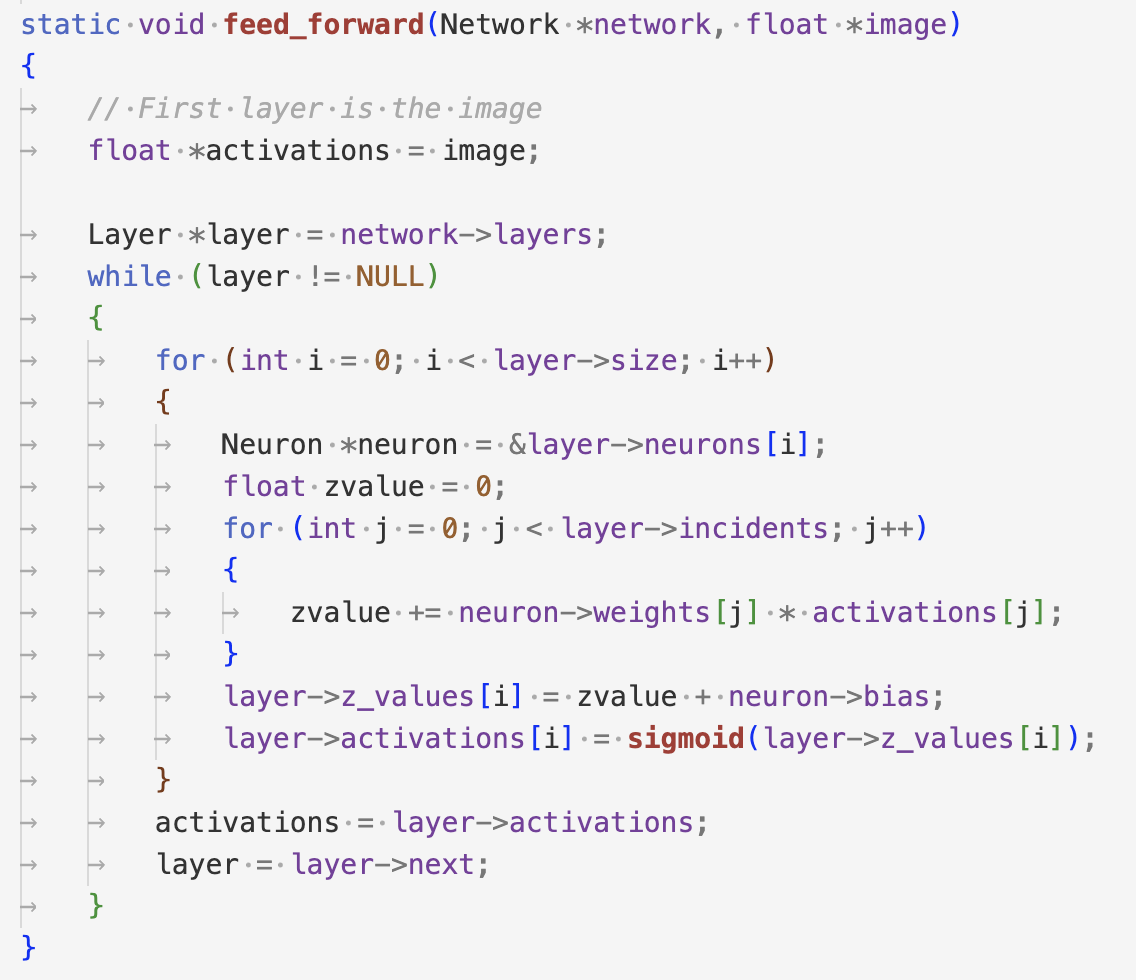
\includegraphics[scale=0.27]{images/c-ff.png}
  \end{figure}

\end{frame}

\begin{frame}
  \frametitle{Accuracy}

  \begin{figure}[!ht]
    \centering
    \scalebox{0.52}{
      %% Creator: Matplotlib, PGF backend
%%
%% To include the figure in your LaTeX document, write
%%   \input{<filename>.pgf}
%%
%% Make sure the required packages are loaded in your preamble
%%   \usepackage{pgf}
%%
%% Also ensure that all the required font packages are loaded; for instance,
%% the lmodern package is sometimes necessary when using math font.
%%   \usepackage{lmodern}
%%
%% Figures using additional raster images can only be included by \input if
%% they are in the same directory as the main LaTeX file. For loading figures
%% from other directories you can use the `import` package
%%   \usepackage{import}
%%
%% and then include the figures with
%%   \import{<path to file>}{<filename>.pgf}
%%
%% Matplotlib used the following preamble
%%   
%%   \usepackage{fontspec}
%%   \setmainfont{Times New Roman.ttf}[Path=\detokenize{/System/Library/Fonts/Supplemental/}]
%%   \setsansfont{DejaVuSans.ttf}[Path=\detokenize{/opt/homebrew/lib/python3.11/site-packages/matplotlib/mpl-data/fonts/ttf/}]
%%   \setmonofont{DejaVuSansMono.ttf}[Path=\detokenize{/opt/homebrew/lib/python3.11/site-packages/matplotlib/mpl-data/fonts/ttf/}]
%%   \makeatletter\@ifpackageloaded{underscore}{}{\usepackage[strings]{underscore}}\makeatother
%%
\begingroup%
\makeatletter%
\begin{pgfpicture}%
\pgfpathrectangle{\pgfpointorigin}{\pgfqpoint{5.916660in}{5.518849in}}%
\pgfusepath{use as bounding box, clip}%
\begin{pgfscope}%
\pgfsetbuttcap%
\pgfsetmiterjoin%
\definecolor{currentfill}{rgb}{1.000000,1.000000,1.000000}%
\pgfsetfillcolor{currentfill}%
\pgfsetlinewidth{0.000000pt}%
\definecolor{currentstroke}{rgb}{1.000000,1.000000,1.000000}%
\pgfsetstrokecolor{currentstroke}%
\pgfsetdash{}{0pt}%
\pgfpathmoveto{\pgfqpoint{0.000000in}{0.000000in}}%
\pgfpathlineto{\pgfqpoint{5.916660in}{0.000000in}}%
\pgfpathlineto{\pgfqpoint{5.916660in}{5.518849in}}%
\pgfpathlineto{\pgfqpoint{0.000000in}{5.518849in}}%
\pgfpathlineto{\pgfqpoint{0.000000in}{0.000000in}}%
\pgfpathclose%
\pgfusepath{fill}%
\end{pgfscope}%
\begin{pgfscope}%
\pgfsetbuttcap%
\pgfsetmiterjoin%
\definecolor{currentfill}{rgb}{1.000000,1.000000,1.000000}%
\pgfsetfillcolor{currentfill}%
\pgfsetlinewidth{0.000000pt}%
\definecolor{currentstroke}{rgb}{0.000000,0.000000,0.000000}%
\pgfsetstrokecolor{currentstroke}%
\pgfsetstrokeopacity{0.000000}%
\pgfsetdash{}{0pt}%
\pgfpathmoveto{\pgfqpoint{0.587522in}{0.323633in}}%
\pgfpathlineto{\pgfqpoint{5.816660in}{0.323633in}}%
\pgfpathlineto{\pgfqpoint{5.816660in}{4.455361in}}%
\pgfpathlineto{\pgfqpoint{0.587522in}{4.455361in}}%
\pgfpathlineto{\pgfqpoint{0.587522in}{0.323633in}}%
\pgfpathclose%
\pgfusepath{fill}%
\end{pgfscope}%
\begin{pgfscope}%
\pgfpathrectangle{\pgfqpoint{0.587522in}{0.323633in}}{\pgfqpoint{5.229138in}{4.131729in}}%
\pgfusepath{clip}%
\pgfsetbuttcap%
\pgfsetmiterjoin%
\definecolor{currentfill}{rgb}{0.509804,0.792157,0.988235}%
\pgfsetfillcolor{currentfill}%
\pgfsetfillopacity{0.810000}%
\pgfsetlinewidth{0.000000pt}%
\definecolor{currentstroke}{rgb}{0.000000,0.000000,0.000000}%
\pgfsetstrokecolor{currentstroke}%
\pgfsetstrokeopacity{0.810000}%
\pgfsetdash{}{0pt}%
\pgfpathmoveto{\pgfqpoint{0.825210in}{0.323633in}}%
\pgfpathlineto{\pgfqpoint{0.947101in}{0.323633in}}%
\pgfpathlineto{\pgfqpoint{0.947101in}{1.571415in}}%
\pgfpathlineto{\pgfqpoint{0.825210in}{1.571415in}}%
\pgfpathlineto{\pgfqpoint{0.825210in}{0.323633in}}%
\pgfpathclose%
\pgfusepath{fill}%
\end{pgfscope}%
\begin{pgfscope}%
\pgfpathrectangle{\pgfqpoint{0.587522in}{0.323633in}}{\pgfqpoint{5.229138in}{4.131729in}}%
\pgfusepath{clip}%
\pgfsetbuttcap%
\pgfsetmiterjoin%
\definecolor{currentfill}{rgb}{0.509804,0.792157,0.988235}%
\pgfsetfillcolor{currentfill}%
\pgfsetfillopacity{0.810000}%
\pgfsetlinewidth{0.000000pt}%
\definecolor{currentstroke}{rgb}{0.000000,0.000000,0.000000}%
\pgfsetstrokecolor{currentstroke}%
\pgfsetstrokeopacity{0.810000}%
\pgfsetdash{}{0pt}%
\pgfpathmoveto{\pgfqpoint{2.044123in}{0.323633in}}%
\pgfpathlineto{\pgfqpoint{2.166014in}{0.323633in}}%
\pgfpathlineto{\pgfqpoint{2.166014in}{1.513571in}}%
\pgfpathlineto{\pgfqpoint{2.044123in}{1.513571in}}%
\pgfpathlineto{\pgfqpoint{2.044123in}{0.323633in}}%
\pgfpathclose%
\pgfusepath{fill}%
\end{pgfscope}%
\begin{pgfscope}%
\pgfpathrectangle{\pgfqpoint{0.587522in}{0.323633in}}{\pgfqpoint{5.229138in}{4.131729in}}%
\pgfusepath{clip}%
\pgfsetbuttcap%
\pgfsetmiterjoin%
\definecolor{currentfill}{rgb}{0.509804,0.792157,0.988235}%
\pgfsetfillcolor{currentfill}%
\pgfsetfillopacity{0.810000}%
\pgfsetlinewidth{0.000000pt}%
\definecolor{currentstroke}{rgb}{0.000000,0.000000,0.000000}%
\pgfsetstrokecolor{currentstroke}%
\pgfsetstrokeopacity{0.810000}%
\pgfsetdash{}{0pt}%
\pgfpathmoveto{\pgfqpoint{3.263036in}{0.323633in}}%
\pgfpathlineto{\pgfqpoint{3.384928in}{0.323633in}}%
\pgfpathlineto{\pgfqpoint{3.384928in}{2.468000in}}%
\pgfpathlineto{\pgfqpoint{3.263036in}{2.468000in}}%
\pgfpathlineto{\pgfqpoint{3.263036in}{0.323633in}}%
\pgfpathclose%
\pgfusepath{fill}%
\end{pgfscope}%
\begin{pgfscope}%
\pgfpathrectangle{\pgfqpoint{0.587522in}{0.323633in}}{\pgfqpoint{5.229138in}{4.131729in}}%
\pgfusepath{clip}%
\pgfsetbuttcap%
\pgfsetmiterjoin%
\definecolor{currentfill}{rgb}{0.509804,0.792157,0.988235}%
\pgfsetfillcolor{currentfill}%
\pgfsetfillopacity{0.810000}%
\pgfsetlinewidth{0.000000pt}%
\definecolor{currentstroke}{rgb}{0.000000,0.000000,0.000000}%
\pgfsetstrokecolor{currentstroke}%
\pgfsetstrokeopacity{0.810000}%
\pgfsetdash{}{0pt}%
\pgfpathmoveto{\pgfqpoint{4.481950in}{0.323633in}}%
\pgfpathlineto{\pgfqpoint{4.603841in}{0.323633in}}%
\pgfpathlineto{\pgfqpoint{4.603841in}{1.856504in}}%
\pgfpathlineto{\pgfqpoint{4.481950in}{1.856504in}}%
\pgfpathlineto{\pgfqpoint{4.481950in}{0.323633in}}%
\pgfpathclose%
\pgfusepath{fill}%
\end{pgfscope}%
\begin{pgfscope}%
\pgfpathrectangle{\pgfqpoint{0.587522in}{0.323633in}}{\pgfqpoint{5.229138in}{4.131729in}}%
\pgfusepath{clip}%
\pgfsetbuttcap%
\pgfsetmiterjoin%
\definecolor{currentfill}{rgb}{1.000000,0.470588,0.333333}%
\pgfsetfillcolor{currentfill}%
\pgfsetfillopacity{0.810000}%
\pgfsetlinewidth{0.000000pt}%
\definecolor{currentstroke}{rgb}{0.000000,0.000000,0.000000}%
\pgfsetstrokecolor{currentstroke}%
\pgfsetstrokeopacity{0.810000}%
\pgfsetdash{}{0pt}%
\pgfpathmoveto{\pgfqpoint{0.947101in}{0.323633in}}%
\pgfpathlineto{\pgfqpoint{1.068992in}{0.323633in}}%
\pgfpathlineto{\pgfqpoint{1.068992in}{2.637401in}}%
\pgfpathlineto{\pgfqpoint{0.947101in}{2.637401in}}%
\pgfpathlineto{\pgfqpoint{0.947101in}{0.323633in}}%
\pgfpathclose%
\pgfusepath{fill}%
\end{pgfscope}%
\begin{pgfscope}%
\pgfpathrectangle{\pgfqpoint{0.587522in}{0.323633in}}{\pgfqpoint{5.229138in}{4.131729in}}%
\pgfusepath{clip}%
\pgfsetbuttcap%
\pgfsetmiterjoin%
\definecolor{currentfill}{rgb}{1.000000,0.470588,0.333333}%
\pgfsetfillcolor{currentfill}%
\pgfsetfillopacity{0.810000}%
\pgfsetlinewidth{0.000000pt}%
\definecolor{currentstroke}{rgb}{0.000000,0.000000,0.000000}%
\pgfsetstrokecolor{currentstroke}%
\pgfsetstrokeopacity{0.810000}%
\pgfsetdash{}{0pt}%
\pgfpathmoveto{\pgfqpoint{2.166014in}{0.323633in}}%
\pgfpathlineto{\pgfqpoint{2.287906in}{0.323633in}}%
\pgfpathlineto{\pgfqpoint{2.287906in}{3.529854in}}%
\pgfpathlineto{\pgfqpoint{2.166014in}{3.529854in}}%
\pgfpathlineto{\pgfqpoint{2.166014in}{0.323633in}}%
\pgfpathclose%
\pgfusepath{fill}%
\end{pgfscope}%
\begin{pgfscope}%
\pgfpathrectangle{\pgfqpoint{0.587522in}{0.323633in}}{\pgfqpoint{5.229138in}{4.131729in}}%
\pgfusepath{clip}%
\pgfsetbuttcap%
\pgfsetmiterjoin%
\definecolor{currentfill}{rgb}{1.000000,0.470588,0.333333}%
\pgfsetfillcolor{currentfill}%
\pgfsetfillopacity{0.810000}%
\pgfsetlinewidth{0.000000pt}%
\definecolor{currentstroke}{rgb}{0.000000,0.000000,0.000000}%
\pgfsetstrokecolor{currentstroke}%
\pgfsetstrokeopacity{0.810000}%
\pgfsetdash{}{0pt}%
\pgfpathmoveto{\pgfqpoint{3.384928in}{0.323633in}}%
\pgfpathlineto{\pgfqpoint{3.506819in}{0.323633in}}%
\pgfpathlineto{\pgfqpoint{3.506819in}{3.038178in}}%
\pgfpathlineto{\pgfqpoint{3.384928in}{3.038178in}}%
\pgfpathlineto{\pgfqpoint{3.384928in}{0.323633in}}%
\pgfpathclose%
\pgfusepath{fill}%
\end{pgfscope}%
\begin{pgfscope}%
\pgfpathrectangle{\pgfqpoint{0.587522in}{0.323633in}}{\pgfqpoint{5.229138in}{4.131729in}}%
\pgfusepath{clip}%
\pgfsetbuttcap%
\pgfsetmiterjoin%
\definecolor{currentfill}{rgb}{1.000000,0.470588,0.333333}%
\pgfsetfillcolor{currentfill}%
\pgfsetfillopacity{0.810000}%
\pgfsetlinewidth{0.000000pt}%
\definecolor{currentstroke}{rgb}{0.000000,0.000000,0.000000}%
\pgfsetstrokecolor{currentstroke}%
\pgfsetstrokeopacity{0.810000}%
\pgfsetdash{}{0pt}%
\pgfpathmoveto{\pgfqpoint{4.603841in}{0.323633in}}%
\pgfpathlineto{\pgfqpoint{4.725733in}{0.323633in}}%
\pgfpathlineto{\pgfqpoint{4.725733in}{2.703508in}}%
\pgfpathlineto{\pgfqpoint{4.603841in}{2.703508in}}%
\pgfpathlineto{\pgfqpoint{4.603841in}{0.323633in}}%
\pgfpathclose%
\pgfusepath{fill}%
\end{pgfscope}%
\begin{pgfscope}%
\pgfpathrectangle{\pgfqpoint{0.587522in}{0.323633in}}{\pgfqpoint{5.229138in}{4.131729in}}%
\pgfusepath{clip}%
\pgfsetbuttcap%
\pgfsetmiterjoin%
\definecolor{currentfill}{rgb}{0.121569,0.654902,0.454902}%
\pgfsetfillcolor{currentfill}%
\pgfsetfillopacity{0.810000}%
\pgfsetlinewidth{0.000000pt}%
\definecolor{currentstroke}{rgb}{0.000000,0.000000,0.000000}%
\pgfsetstrokecolor{currentstroke}%
\pgfsetstrokeopacity{0.810000}%
\pgfsetdash{}{0pt}%
\pgfpathmoveto{\pgfqpoint{1.068992in}{0.323633in}}%
\pgfpathlineto{\pgfqpoint{1.190884in}{0.323633in}}%
\pgfpathlineto{\pgfqpoint{1.190884in}{3.971949in}}%
\pgfpathlineto{\pgfqpoint{1.068992in}{3.971949in}}%
\pgfpathlineto{\pgfqpoint{1.068992in}{0.323633in}}%
\pgfpathclose%
\pgfusepath{fill}%
\end{pgfscope}%
\begin{pgfscope}%
\pgfpathrectangle{\pgfqpoint{0.587522in}{0.323633in}}{\pgfqpoint{5.229138in}{4.131729in}}%
\pgfusepath{clip}%
\pgfsetbuttcap%
\pgfsetmiterjoin%
\definecolor{currentfill}{rgb}{0.121569,0.654902,0.454902}%
\pgfsetfillcolor{currentfill}%
\pgfsetfillopacity{0.810000}%
\pgfsetlinewidth{0.000000pt}%
\definecolor{currentstroke}{rgb}{0.000000,0.000000,0.000000}%
\pgfsetstrokecolor{currentstroke}%
\pgfsetstrokeopacity{0.810000}%
\pgfsetdash{}{0pt}%
\pgfpathmoveto{\pgfqpoint{2.287906in}{0.323633in}}%
\pgfpathlineto{\pgfqpoint{2.409797in}{0.323633in}}%
\pgfpathlineto{\pgfqpoint{2.409797in}{3.922368in}}%
\pgfpathlineto{\pgfqpoint{2.287906in}{3.922368in}}%
\pgfpathlineto{\pgfqpoint{2.287906in}{0.323633in}}%
\pgfpathclose%
\pgfusepath{fill}%
\end{pgfscope}%
\begin{pgfscope}%
\pgfpathrectangle{\pgfqpoint{0.587522in}{0.323633in}}{\pgfqpoint{5.229138in}{4.131729in}}%
\pgfusepath{clip}%
\pgfsetbuttcap%
\pgfsetmiterjoin%
\definecolor{currentfill}{rgb}{0.121569,0.654902,0.454902}%
\pgfsetfillcolor{currentfill}%
\pgfsetfillopacity{0.810000}%
\pgfsetlinewidth{0.000000pt}%
\definecolor{currentstroke}{rgb}{0.000000,0.000000,0.000000}%
\pgfsetstrokecolor{currentstroke}%
\pgfsetstrokeopacity{0.810000}%
\pgfsetdash{}{0pt}%
\pgfpathmoveto{\pgfqpoint{3.506819in}{0.323633in}}%
\pgfpathlineto{\pgfqpoint{3.628710in}{0.323633in}}%
\pgfpathlineto{\pgfqpoint{3.628710in}{4.079374in}}%
\pgfpathlineto{\pgfqpoint{3.506819in}{4.079374in}}%
\pgfpathlineto{\pgfqpoint{3.506819in}{0.323633in}}%
\pgfpathclose%
\pgfusepath{fill}%
\end{pgfscope}%
\begin{pgfscope}%
\pgfpathrectangle{\pgfqpoint{0.587522in}{0.323633in}}{\pgfqpoint{5.229138in}{4.131729in}}%
\pgfusepath{clip}%
\pgfsetbuttcap%
\pgfsetmiterjoin%
\definecolor{currentfill}{rgb}{0.121569,0.654902,0.454902}%
\pgfsetfillcolor{currentfill}%
\pgfsetfillopacity{0.810000}%
\pgfsetlinewidth{0.000000pt}%
\definecolor{currentstroke}{rgb}{0.000000,0.000000,0.000000}%
\pgfsetstrokecolor{currentstroke}%
\pgfsetstrokeopacity{0.810000}%
\pgfsetdash{}{0pt}%
\pgfpathmoveto{\pgfqpoint{4.725733in}{0.323633in}}%
\pgfpathlineto{\pgfqpoint{4.847624in}{0.323633in}}%
\pgfpathlineto{\pgfqpoint{4.847624in}{3.996740in}}%
\pgfpathlineto{\pgfqpoint{4.725733in}{3.996740in}}%
\pgfpathlineto{\pgfqpoint{4.725733in}{0.323633in}}%
\pgfpathclose%
\pgfusepath{fill}%
\end{pgfscope}%
\begin{pgfscope}%
\pgfpathrectangle{\pgfqpoint{0.587522in}{0.323633in}}{\pgfqpoint{5.229138in}{4.131729in}}%
\pgfusepath{clip}%
\pgfsetbuttcap%
\pgfsetmiterjoin%
\definecolor{currentfill}{rgb}{0.984314,0.160784,0.262745}%
\pgfsetfillcolor{currentfill}%
\pgfsetfillopacity{0.810000}%
\pgfsetlinewidth{0.000000pt}%
\definecolor{currentstroke}{rgb}{0.000000,0.000000,0.000000}%
\pgfsetstrokecolor{currentstroke}%
\pgfsetstrokeopacity{0.810000}%
\pgfsetdash{}{0pt}%
\pgfpathmoveto{\pgfqpoint{1.190884in}{0.323633in}}%
\pgfpathlineto{\pgfqpoint{1.312775in}{0.323633in}}%
\pgfpathlineto{\pgfqpoint{1.312775in}{4.120691in}}%
\pgfpathlineto{\pgfqpoint{1.190884in}{4.120691in}}%
\pgfpathlineto{\pgfqpoint{1.190884in}{0.323633in}}%
\pgfpathclose%
\pgfusepath{fill}%
\end{pgfscope}%
\begin{pgfscope}%
\pgfpathrectangle{\pgfqpoint{0.587522in}{0.323633in}}{\pgfqpoint{5.229138in}{4.131729in}}%
\pgfusepath{clip}%
\pgfsetbuttcap%
\pgfsetmiterjoin%
\definecolor{currentfill}{rgb}{0.984314,0.160784,0.262745}%
\pgfsetfillcolor{currentfill}%
\pgfsetfillopacity{0.810000}%
\pgfsetlinewidth{0.000000pt}%
\definecolor{currentstroke}{rgb}{0.000000,0.000000,0.000000}%
\pgfsetstrokecolor{currentstroke}%
\pgfsetstrokeopacity{0.810000}%
\pgfsetdash{}{0pt}%
\pgfpathmoveto{\pgfqpoint{2.409797in}{0.323633in}}%
\pgfpathlineto{\pgfqpoint{2.531688in}{0.323633in}}%
\pgfpathlineto{\pgfqpoint{2.531688in}{4.112428in}}%
\pgfpathlineto{\pgfqpoint{2.409797in}{4.112428in}}%
\pgfpathlineto{\pgfqpoint{2.409797in}{0.323633in}}%
\pgfpathclose%
\pgfusepath{fill}%
\end{pgfscope}%
\begin{pgfscope}%
\pgfpathrectangle{\pgfqpoint{0.587522in}{0.323633in}}{\pgfqpoint{5.229138in}{4.131729in}}%
\pgfusepath{clip}%
\pgfsetbuttcap%
\pgfsetmiterjoin%
\definecolor{currentfill}{rgb}{0.984314,0.160784,0.262745}%
\pgfsetfillcolor{currentfill}%
\pgfsetfillopacity{0.810000}%
\pgfsetlinewidth{0.000000pt}%
\definecolor{currentstroke}{rgb}{0.000000,0.000000,0.000000}%
\pgfsetstrokecolor{currentstroke}%
\pgfsetstrokeopacity{0.810000}%
\pgfsetdash{}{0pt}%
\pgfpathmoveto{\pgfqpoint{3.628710in}{0.323633in}}%
\pgfpathlineto{\pgfqpoint{3.750602in}{0.323633in}}%
\pgfpathlineto{\pgfqpoint{3.750602in}{4.190931in}}%
\pgfpathlineto{\pgfqpoint{3.628710in}{4.190931in}}%
\pgfpathlineto{\pgfqpoint{3.628710in}{0.323633in}}%
\pgfpathclose%
\pgfusepath{fill}%
\end{pgfscope}%
\begin{pgfscope}%
\pgfpathrectangle{\pgfqpoint{0.587522in}{0.323633in}}{\pgfqpoint{5.229138in}{4.131729in}}%
\pgfusepath{clip}%
\pgfsetbuttcap%
\pgfsetmiterjoin%
\definecolor{currentfill}{rgb}{0.984314,0.160784,0.262745}%
\pgfsetfillcolor{currentfill}%
\pgfsetfillopacity{0.810000}%
\pgfsetlinewidth{0.000000pt}%
\definecolor{currentstroke}{rgb}{0.000000,0.000000,0.000000}%
\pgfsetstrokecolor{currentstroke}%
\pgfsetstrokeopacity{0.810000}%
\pgfsetdash{}{0pt}%
\pgfpathmoveto{\pgfqpoint{4.847624in}{0.323633in}}%
\pgfpathlineto{\pgfqpoint{4.969515in}{0.323633in}}%
\pgfpathlineto{\pgfqpoint{4.969515in}{4.124823in}}%
\pgfpathlineto{\pgfqpoint{4.847624in}{4.124823in}}%
\pgfpathlineto{\pgfqpoint{4.847624in}{0.323633in}}%
\pgfpathclose%
\pgfusepath{fill}%
\end{pgfscope}%
\begin{pgfscope}%
\pgfpathrectangle{\pgfqpoint{0.587522in}{0.323633in}}{\pgfqpoint{5.229138in}{4.131729in}}%
\pgfusepath{clip}%
\pgfsetbuttcap%
\pgfsetmiterjoin%
\definecolor{currentfill}{rgb}{0.607843,0.372549,0.752941}%
\pgfsetfillcolor{currentfill}%
\pgfsetfillopacity{0.810000}%
\pgfsetlinewidth{0.000000pt}%
\definecolor{currentstroke}{rgb}{0.000000,0.000000,0.000000}%
\pgfsetstrokecolor{currentstroke}%
\pgfsetstrokeopacity{0.810000}%
\pgfsetdash{}{0pt}%
\pgfpathmoveto{\pgfqpoint{1.312775in}{0.323633in}}%
\pgfpathlineto{\pgfqpoint{1.434666in}{0.323633in}}%
\pgfpathlineto{\pgfqpoint{1.434666in}{4.211589in}}%
\pgfpathlineto{\pgfqpoint{1.312775in}{4.211589in}}%
\pgfpathlineto{\pgfqpoint{1.312775in}{0.323633in}}%
\pgfpathclose%
\pgfusepath{fill}%
\end{pgfscope}%
\begin{pgfscope}%
\pgfpathrectangle{\pgfqpoint{0.587522in}{0.323633in}}{\pgfqpoint{5.229138in}{4.131729in}}%
\pgfusepath{clip}%
\pgfsetbuttcap%
\pgfsetmiterjoin%
\definecolor{currentfill}{rgb}{0.607843,0.372549,0.752941}%
\pgfsetfillcolor{currentfill}%
\pgfsetfillopacity{0.810000}%
\pgfsetlinewidth{0.000000pt}%
\definecolor{currentstroke}{rgb}{0.000000,0.000000,0.000000}%
\pgfsetstrokecolor{currentstroke}%
\pgfsetstrokeopacity{0.810000}%
\pgfsetdash{}{0pt}%
\pgfpathmoveto{\pgfqpoint{2.531688in}{0.323633in}}%
\pgfpathlineto{\pgfqpoint{2.653580in}{0.323633in}}%
\pgfpathlineto{\pgfqpoint{2.653580in}{4.203326in}}%
\pgfpathlineto{\pgfqpoint{2.531688in}{4.203326in}}%
\pgfpathlineto{\pgfqpoint{2.531688in}{0.323633in}}%
\pgfpathclose%
\pgfusepath{fill}%
\end{pgfscope}%
\begin{pgfscope}%
\pgfpathrectangle{\pgfqpoint{0.587522in}{0.323633in}}{\pgfqpoint{5.229138in}{4.131729in}}%
\pgfusepath{clip}%
\pgfsetbuttcap%
\pgfsetmiterjoin%
\definecolor{currentfill}{rgb}{0.607843,0.372549,0.752941}%
\pgfsetfillcolor{currentfill}%
\pgfsetfillopacity{0.810000}%
\pgfsetlinewidth{0.000000pt}%
\definecolor{currentstroke}{rgb}{0.000000,0.000000,0.000000}%
\pgfsetstrokecolor{currentstroke}%
\pgfsetstrokeopacity{0.810000}%
\pgfsetdash{}{0pt}%
\pgfpathmoveto{\pgfqpoint{3.750602in}{0.323633in}}%
\pgfpathlineto{\pgfqpoint{3.872493in}{0.323633in}}%
\pgfpathlineto{\pgfqpoint{3.872493in}{4.265302in}}%
\pgfpathlineto{\pgfqpoint{3.750602in}{4.265302in}}%
\pgfpathlineto{\pgfqpoint{3.750602in}{0.323633in}}%
\pgfpathclose%
\pgfusepath{fill}%
\end{pgfscope}%
\begin{pgfscope}%
\pgfpathrectangle{\pgfqpoint{0.587522in}{0.323633in}}{\pgfqpoint{5.229138in}{4.131729in}}%
\pgfusepath{clip}%
\pgfsetbuttcap%
\pgfsetmiterjoin%
\definecolor{currentfill}{rgb}{0.607843,0.372549,0.752941}%
\pgfsetfillcolor{currentfill}%
\pgfsetfillopacity{0.810000}%
\pgfsetlinewidth{0.000000pt}%
\definecolor{currentstroke}{rgb}{0.000000,0.000000,0.000000}%
\pgfsetstrokecolor{currentstroke}%
\pgfsetstrokeopacity{0.810000}%
\pgfsetdash{}{0pt}%
\pgfpathmoveto{\pgfqpoint{4.969515in}{0.323633in}}%
\pgfpathlineto{\pgfqpoint{5.091407in}{0.323633in}}%
\pgfpathlineto{\pgfqpoint{5.091407in}{3.847997in}}%
\pgfpathlineto{\pgfqpoint{4.969515in}{3.847997in}}%
\pgfpathlineto{\pgfqpoint{4.969515in}{0.323633in}}%
\pgfpathclose%
\pgfusepath{fill}%
\end{pgfscope}%
\begin{pgfscope}%
\pgfpathrectangle{\pgfqpoint{0.587522in}{0.323633in}}{\pgfqpoint{5.229138in}{4.131729in}}%
\pgfusepath{clip}%
\pgfsetbuttcap%
\pgfsetmiterjoin%
\definecolor{currentfill}{rgb}{0.529412,0.372549,0.258824}%
\pgfsetfillcolor{currentfill}%
\pgfsetfillopacity{0.810000}%
\pgfsetlinewidth{0.000000pt}%
\definecolor{currentstroke}{rgb}{0.000000,0.000000,0.000000}%
\pgfsetstrokecolor{currentstroke}%
\pgfsetstrokeopacity{0.810000}%
\pgfsetdash{}{0pt}%
\pgfpathmoveto{\pgfqpoint{1.434666in}{0.323633in}}%
\pgfpathlineto{\pgfqpoint{1.556558in}{0.323633in}}%
\pgfpathlineto{\pgfqpoint{1.556558in}{4.100033in}}%
\pgfpathlineto{\pgfqpoint{1.434666in}{4.100033in}}%
\pgfpathlineto{\pgfqpoint{1.434666in}{0.323633in}}%
\pgfpathclose%
\pgfusepath{fill}%
\end{pgfscope}%
\begin{pgfscope}%
\pgfpathrectangle{\pgfqpoint{0.587522in}{0.323633in}}{\pgfqpoint{5.229138in}{4.131729in}}%
\pgfusepath{clip}%
\pgfsetbuttcap%
\pgfsetmiterjoin%
\definecolor{currentfill}{rgb}{0.529412,0.372549,0.258824}%
\pgfsetfillcolor{currentfill}%
\pgfsetfillopacity{0.810000}%
\pgfsetlinewidth{0.000000pt}%
\definecolor{currentstroke}{rgb}{0.000000,0.000000,0.000000}%
\pgfsetstrokecolor{currentstroke}%
\pgfsetstrokeopacity{0.810000}%
\pgfsetdash{}{0pt}%
\pgfpathmoveto{\pgfqpoint{2.653580in}{0.323633in}}%
\pgfpathlineto{\pgfqpoint{2.775471in}{0.323633in}}%
\pgfpathlineto{\pgfqpoint{2.775471in}{4.182667in}}%
\pgfpathlineto{\pgfqpoint{2.653580in}{4.182667in}}%
\pgfpathlineto{\pgfqpoint{2.653580in}{0.323633in}}%
\pgfpathclose%
\pgfusepath{fill}%
\end{pgfscope}%
\begin{pgfscope}%
\pgfpathrectangle{\pgfqpoint{0.587522in}{0.323633in}}{\pgfqpoint{5.229138in}{4.131729in}}%
\pgfusepath{clip}%
\pgfsetbuttcap%
\pgfsetmiterjoin%
\definecolor{currentfill}{rgb}{0.529412,0.372549,0.258824}%
\pgfsetfillcolor{currentfill}%
\pgfsetfillopacity{0.810000}%
\pgfsetlinewidth{0.000000pt}%
\definecolor{currentstroke}{rgb}{0.000000,0.000000,0.000000}%
\pgfsetstrokecolor{currentstroke}%
\pgfsetstrokeopacity{0.810000}%
\pgfsetdash{}{0pt}%
\pgfpathmoveto{\pgfqpoint{3.872493in}{0.323633in}}%
\pgfpathlineto{\pgfqpoint{3.994384in}{0.323633in}}%
\pgfpathlineto{\pgfqpoint{3.994384in}{4.025662in}}%
\pgfpathlineto{\pgfqpoint{3.872493in}{4.025662in}}%
\pgfpathlineto{\pgfqpoint{3.872493in}{0.323633in}}%
\pgfpathclose%
\pgfusepath{fill}%
\end{pgfscope}%
\begin{pgfscope}%
\pgfpathrectangle{\pgfqpoint{0.587522in}{0.323633in}}{\pgfqpoint{5.229138in}{4.131729in}}%
\pgfusepath{clip}%
\pgfsetbuttcap%
\pgfsetmiterjoin%
\definecolor{currentfill}{rgb}{0.529412,0.372549,0.258824}%
\pgfsetfillcolor{currentfill}%
\pgfsetfillopacity{0.810000}%
\pgfsetlinewidth{0.000000pt}%
\definecolor{currentstroke}{rgb}{0.000000,0.000000,0.000000}%
\pgfsetstrokecolor{currentstroke}%
\pgfsetstrokeopacity{0.810000}%
\pgfsetdash{}{0pt}%
\pgfpathmoveto{\pgfqpoint{5.091407in}{0.323633in}}%
\pgfpathlineto{\pgfqpoint{5.213298in}{0.323633in}}%
\pgfpathlineto{\pgfqpoint{5.213298in}{4.178536in}}%
\pgfpathlineto{\pgfqpoint{5.091407in}{4.178536in}}%
\pgfpathlineto{\pgfqpoint{5.091407in}{0.323633in}}%
\pgfpathclose%
\pgfusepath{fill}%
\end{pgfscope}%
\begin{pgfscope}%
\pgfpathrectangle{\pgfqpoint{0.587522in}{0.323633in}}{\pgfqpoint{5.229138in}{4.131729in}}%
\pgfusepath{clip}%
\pgfsetbuttcap%
\pgfsetmiterjoin%
\definecolor{currentfill}{rgb}{0.964706,0.407843,0.556863}%
\pgfsetfillcolor{currentfill}%
\pgfsetfillopacity{0.810000}%
\pgfsetlinewidth{0.000000pt}%
\definecolor{currentstroke}{rgb}{0.000000,0.000000,0.000000}%
\pgfsetstrokecolor{currentstroke}%
\pgfsetstrokeopacity{0.810000}%
\pgfsetdash{}{0pt}%
\pgfpathmoveto{\pgfqpoint{1.556558in}{0.323633in}}%
\pgfpathlineto{\pgfqpoint{1.678449in}{0.323633in}}%
\pgfpathlineto{\pgfqpoint{1.678449in}{3.823207in}}%
\pgfpathlineto{\pgfqpoint{1.556558in}{3.823207in}}%
\pgfpathlineto{\pgfqpoint{1.556558in}{0.323633in}}%
\pgfpathclose%
\pgfusepath{fill}%
\end{pgfscope}%
\begin{pgfscope}%
\pgfpathrectangle{\pgfqpoint{0.587522in}{0.323633in}}{\pgfqpoint{5.229138in}{4.131729in}}%
\pgfusepath{clip}%
\pgfsetbuttcap%
\pgfsetmiterjoin%
\definecolor{currentfill}{rgb}{0.964706,0.407843,0.556863}%
\pgfsetfillcolor{currentfill}%
\pgfsetfillopacity{0.810000}%
\pgfsetlinewidth{0.000000pt}%
\definecolor{currentstroke}{rgb}{0.000000,0.000000,0.000000}%
\pgfsetstrokecolor{currentstroke}%
\pgfsetstrokeopacity{0.810000}%
\pgfsetdash{}{0pt}%
\pgfpathmoveto{\pgfqpoint{2.775471in}{0.323633in}}%
\pgfpathlineto{\pgfqpoint{2.897362in}{0.323633in}}%
\pgfpathlineto{\pgfqpoint{2.897362in}{4.240512in}}%
\pgfpathlineto{\pgfqpoint{2.775471in}{4.240512in}}%
\pgfpathlineto{\pgfqpoint{2.775471in}{0.323633in}}%
\pgfpathclose%
\pgfusepath{fill}%
\end{pgfscope}%
\begin{pgfscope}%
\pgfpathrectangle{\pgfqpoint{0.587522in}{0.323633in}}{\pgfqpoint{5.229138in}{4.131729in}}%
\pgfusepath{clip}%
\pgfsetbuttcap%
\pgfsetmiterjoin%
\definecolor{currentfill}{rgb}{0.964706,0.407843,0.556863}%
\pgfsetfillcolor{currentfill}%
\pgfsetfillopacity{0.810000}%
\pgfsetlinewidth{0.000000pt}%
\definecolor{currentstroke}{rgb}{0.000000,0.000000,0.000000}%
\pgfsetstrokecolor{currentstroke}%
\pgfsetstrokeopacity{0.810000}%
\pgfsetdash{}{0pt}%
\pgfpathmoveto{\pgfqpoint{3.994384in}{0.323633in}}%
\pgfpathlineto{\pgfqpoint{4.116276in}{0.323633in}}%
\pgfpathlineto{\pgfqpoint{4.116276in}{4.298356in}}%
\pgfpathlineto{\pgfqpoint{3.994384in}{4.298356in}}%
\pgfpathlineto{\pgfqpoint{3.994384in}{0.323633in}}%
\pgfpathclose%
\pgfusepath{fill}%
\end{pgfscope}%
\begin{pgfscope}%
\pgfpathrectangle{\pgfqpoint{0.587522in}{0.323633in}}{\pgfqpoint{5.229138in}{4.131729in}}%
\pgfusepath{clip}%
\pgfsetbuttcap%
\pgfsetmiterjoin%
\definecolor{currentfill}{rgb}{0.964706,0.407843,0.556863}%
\pgfsetfillcolor{currentfill}%
\pgfsetfillopacity{0.810000}%
\pgfsetlinewidth{0.000000pt}%
\definecolor{currentstroke}{rgb}{0.000000,0.000000,0.000000}%
\pgfsetstrokecolor{currentstroke}%
\pgfsetstrokeopacity{0.810000}%
\pgfsetdash{}{0pt}%
\pgfpathmoveto{\pgfqpoint{5.213298in}{0.323633in}}%
\pgfpathlineto{\pgfqpoint{5.335189in}{0.323633in}}%
\pgfpathlineto{\pgfqpoint{5.335189in}{4.211589in}}%
\pgfpathlineto{\pgfqpoint{5.213298in}{4.211589in}}%
\pgfpathlineto{\pgfqpoint{5.213298in}{0.323633in}}%
\pgfpathclose%
\pgfusepath{fill}%
\end{pgfscope}%
\begin{pgfscope}%
\pgfpathrectangle{\pgfqpoint{0.587522in}{0.323633in}}{\pgfqpoint{5.229138in}{4.131729in}}%
\pgfusepath{clip}%
\pgfsetbuttcap%
\pgfsetmiterjoin%
\definecolor{currentfill}{rgb}{0.450980,0.290196,0.396078}%
\pgfsetfillcolor{currentfill}%
\pgfsetfillopacity{0.810000}%
\pgfsetlinewidth{0.000000pt}%
\definecolor{currentstroke}{rgb}{0.000000,0.000000,0.000000}%
\pgfsetstrokecolor{currentstroke}%
\pgfsetstrokeopacity{0.810000}%
\pgfsetdash{}{0pt}%
\pgfpathmoveto{\pgfqpoint{1.678449in}{0.323633in}}%
\pgfpathlineto{\pgfqpoint{1.800340in}{0.323633in}}%
\pgfpathlineto{\pgfqpoint{1.800340in}{3.819075in}}%
\pgfpathlineto{\pgfqpoint{1.678449in}{3.819075in}}%
\pgfpathlineto{\pgfqpoint{1.678449in}{0.323633in}}%
\pgfpathclose%
\pgfusepath{fill}%
\end{pgfscope}%
\begin{pgfscope}%
\pgfpathrectangle{\pgfqpoint{0.587522in}{0.323633in}}{\pgfqpoint{5.229138in}{4.131729in}}%
\pgfusepath{clip}%
\pgfsetbuttcap%
\pgfsetmiterjoin%
\definecolor{currentfill}{rgb}{0.450980,0.290196,0.396078}%
\pgfsetfillcolor{currentfill}%
\pgfsetfillopacity{0.810000}%
\pgfsetlinewidth{0.000000pt}%
\definecolor{currentstroke}{rgb}{0.000000,0.000000,0.000000}%
\pgfsetstrokecolor{currentstroke}%
\pgfsetstrokeopacity{0.810000}%
\pgfsetdash{}{0pt}%
\pgfpathmoveto{\pgfqpoint{2.897362in}{0.323633in}}%
\pgfpathlineto{\pgfqpoint{3.019254in}{0.323633in}}%
\pgfpathlineto{\pgfqpoint{3.019254in}{4.203326in}}%
\pgfpathlineto{\pgfqpoint{2.897362in}{4.203326in}}%
\pgfpathlineto{\pgfqpoint{2.897362in}{0.323633in}}%
\pgfpathclose%
\pgfusepath{fill}%
\end{pgfscope}%
\begin{pgfscope}%
\pgfpathrectangle{\pgfqpoint{0.587522in}{0.323633in}}{\pgfqpoint{5.229138in}{4.131729in}}%
\pgfusepath{clip}%
\pgfsetbuttcap%
\pgfsetmiterjoin%
\definecolor{currentfill}{rgb}{0.450980,0.290196,0.396078}%
\pgfsetfillcolor{currentfill}%
\pgfsetfillopacity{0.810000}%
\pgfsetlinewidth{0.000000pt}%
\definecolor{currentstroke}{rgb}{0.000000,0.000000,0.000000}%
\pgfsetstrokecolor{currentstroke}%
\pgfsetstrokeopacity{0.810000}%
\pgfsetdash{}{0pt}%
\pgfpathmoveto{\pgfqpoint{4.116276in}{0.323633in}}%
\pgfpathlineto{\pgfqpoint{4.238167in}{0.323633in}}%
\pgfpathlineto{\pgfqpoint{4.238167in}{4.310751in}}%
\pgfpathlineto{\pgfqpoint{4.116276in}{4.310751in}}%
\pgfpathlineto{\pgfqpoint{4.116276in}{0.323633in}}%
\pgfpathclose%
\pgfusepath{fill}%
\end{pgfscope}%
\begin{pgfscope}%
\pgfpathrectangle{\pgfqpoint{0.587522in}{0.323633in}}{\pgfqpoint{5.229138in}{4.131729in}}%
\pgfusepath{clip}%
\pgfsetbuttcap%
\pgfsetmiterjoin%
\definecolor{currentfill}{rgb}{0.450980,0.290196,0.396078}%
\pgfsetfillcolor{currentfill}%
\pgfsetfillopacity{0.810000}%
\pgfsetlinewidth{0.000000pt}%
\definecolor{currentstroke}{rgb}{0.000000,0.000000,0.000000}%
\pgfsetstrokecolor{currentstroke}%
\pgfsetstrokeopacity{0.810000}%
\pgfsetdash{}{0pt}%
\pgfpathmoveto{\pgfqpoint{5.335189in}{0.323633in}}%
\pgfpathlineto{\pgfqpoint{5.457081in}{0.323633in}}%
\pgfpathlineto{\pgfqpoint{5.457081in}{3.352190in}}%
\pgfpathlineto{\pgfqpoint{5.335189in}{3.352190in}}%
\pgfpathlineto{\pgfqpoint{5.335189in}{0.323633in}}%
\pgfpathclose%
\pgfusepath{fill}%
\end{pgfscope}%
\begin{pgfscope}%
\pgfpathrectangle{\pgfqpoint{0.587522in}{0.323633in}}{\pgfqpoint{5.229138in}{4.131729in}}%
\pgfusepath{clip}%
\pgfsetbuttcap%
\pgfsetmiterjoin%
\definecolor{currentfill}{rgb}{0.678431,0.647059,0.529412}%
\pgfsetfillcolor{currentfill}%
\pgfsetfillopacity{0.810000}%
\pgfsetlinewidth{0.000000pt}%
\definecolor{currentstroke}{rgb}{0.000000,0.000000,0.000000}%
\pgfsetstrokecolor{currentstroke}%
\pgfsetstrokeopacity{0.810000}%
\pgfsetdash{}{0pt}%
\pgfpathmoveto{\pgfqpoint{1.800340in}{0.323633in}}%
\pgfpathlineto{\pgfqpoint{1.922232in}{0.323633in}}%
\pgfpathlineto{\pgfqpoint{1.922232in}{3.405902in}}%
\pgfpathlineto{\pgfqpoint{1.800340in}{3.405902in}}%
\pgfpathlineto{\pgfqpoint{1.800340in}{0.323633in}}%
\pgfpathclose%
\pgfusepath{fill}%
\end{pgfscope}%
\begin{pgfscope}%
\pgfpathrectangle{\pgfqpoint{0.587522in}{0.323633in}}{\pgfqpoint{5.229138in}{4.131729in}}%
\pgfusepath{clip}%
\pgfsetbuttcap%
\pgfsetmiterjoin%
\definecolor{currentfill}{rgb}{0.678431,0.647059,0.529412}%
\pgfsetfillcolor{currentfill}%
\pgfsetfillopacity{0.810000}%
\pgfsetlinewidth{0.000000pt}%
\definecolor{currentstroke}{rgb}{0.000000,0.000000,0.000000}%
\pgfsetstrokecolor{currentstroke}%
\pgfsetstrokeopacity{0.810000}%
\pgfsetdash{}{0pt}%
\pgfpathmoveto{\pgfqpoint{3.019254in}{0.323633in}}%
\pgfpathlineto{\pgfqpoint{3.141145in}{0.323633in}}%
\pgfpathlineto{\pgfqpoint{3.141145in}{3.021652in}}%
\pgfpathlineto{\pgfqpoint{3.019254in}{3.021652in}}%
\pgfpathlineto{\pgfqpoint{3.019254in}{0.323633in}}%
\pgfpathclose%
\pgfusepath{fill}%
\end{pgfscope}%
\begin{pgfscope}%
\pgfpathrectangle{\pgfqpoint{0.587522in}{0.323633in}}{\pgfqpoint{5.229138in}{4.131729in}}%
\pgfusepath{clip}%
\pgfsetbuttcap%
\pgfsetmiterjoin%
\definecolor{currentfill}{rgb}{0.678431,0.647059,0.529412}%
\pgfsetfillcolor{currentfill}%
\pgfsetfillopacity{0.810000}%
\pgfsetlinewidth{0.000000pt}%
\definecolor{currentstroke}{rgb}{0.000000,0.000000,0.000000}%
\pgfsetstrokecolor{currentstroke}%
\pgfsetstrokeopacity{0.810000}%
\pgfsetdash{}{0pt}%
\pgfpathmoveto{\pgfqpoint{4.238167in}{0.323633in}}%
\pgfpathlineto{\pgfqpoint{4.360058in}{0.323633in}}%
\pgfpathlineto{\pgfqpoint{4.360058in}{4.310751in}}%
\pgfpathlineto{\pgfqpoint{4.238167in}{4.310751in}}%
\pgfpathlineto{\pgfqpoint{4.238167in}{0.323633in}}%
\pgfpathclose%
\pgfusepath{fill}%
\end{pgfscope}%
\begin{pgfscope}%
\pgfpathrectangle{\pgfqpoint{0.587522in}{0.323633in}}{\pgfqpoint{5.229138in}{4.131729in}}%
\pgfusepath{clip}%
\pgfsetbuttcap%
\pgfsetmiterjoin%
\definecolor{currentfill}{rgb}{0.678431,0.647059,0.529412}%
\pgfsetfillcolor{currentfill}%
\pgfsetfillopacity{0.810000}%
\pgfsetlinewidth{0.000000pt}%
\definecolor{currentstroke}{rgb}{0.000000,0.000000,0.000000}%
\pgfsetstrokecolor{currentstroke}%
\pgfsetstrokeopacity{0.810000}%
\pgfsetdash{}{0pt}%
\pgfpathmoveto{\pgfqpoint{5.457081in}{0.323633in}}%
\pgfpathlineto{\pgfqpoint{5.578972in}{0.323633in}}%
\pgfpathlineto{\pgfqpoint{5.578972in}{4.124823in}}%
\pgfpathlineto{\pgfqpoint{5.457081in}{4.124823in}}%
\pgfpathlineto{\pgfqpoint{5.457081in}{0.323633in}}%
\pgfpathclose%
\pgfusepath{fill}%
\end{pgfscope}%
\begin{pgfscope}%
\pgfsetbuttcap%
\pgfsetroundjoin%
\definecolor{currentfill}{rgb}{0.000000,0.000000,0.000000}%
\pgfsetfillcolor{currentfill}%
\pgfsetlinewidth{0.803000pt}%
\definecolor{currentstroke}{rgb}{0.000000,0.000000,0.000000}%
\pgfsetstrokecolor{currentstroke}%
\pgfsetdash{}{0pt}%
\pgfsys@defobject{currentmarker}{\pgfqpoint{0.000000in}{-0.048611in}}{\pgfqpoint{0.000000in}{0.000000in}}{%
\pgfpathmoveto{\pgfqpoint{0.000000in}{0.000000in}}%
\pgfpathlineto{\pgfqpoint{0.000000in}{-0.048611in}}%
\pgfusepath{stroke,fill}%
}%
\begin{pgfscope}%
\pgfsys@transformshift{1.373721in}{0.323633in}%
\pgfsys@useobject{currentmarker}{}%
\end{pgfscope}%
\end{pgfscope}%
\begin{pgfscope}%
\definecolor{textcolor}{rgb}{0.000000,0.000000,0.000000}%
\pgfsetstrokecolor{textcolor}%
\pgfsetfillcolor{textcolor}%
\pgftext[x=1.373721in,y=0.226410in,,top]{\color{textcolor}\rmfamily\fontsize{10.000000}{12.000000}\selectfont c-math.h}%
\end{pgfscope}%
\begin{pgfscope}%
\pgfsetbuttcap%
\pgfsetroundjoin%
\definecolor{currentfill}{rgb}{0.000000,0.000000,0.000000}%
\pgfsetfillcolor{currentfill}%
\pgfsetlinewidth{0.803000pt}%
\definecolor{currentstroke}{rgb}{0.000000,0.000000,0.000000}%
\pgfsetstrokecolor{currentstroke}%
\pgfsetdash{}{0pt}%
\pgfsys@defobject{currentmarker}{\pgfqpoint{0.000000in}{-0.048611in}}{\pgfqpoint{0.000000in}{0.000000in}}{%
\pgfpathmoveto{\pgfqpoint{0.000000in}{0.000000in}}%
\pgfpathlineto{\pgfqpoint{0.000000in}{-0.048611in}}%
\pgfusepath{stroke,fill}%
}%
\begin{pgfscope}%
\pgfsys@transformshift{2.592634in}{0.323633in}%
\pgfsys@useobject{currentmarker}{}%
\end{pgfscope}%
\end{pgfscope}%
\begin{pgfscope}%
\definecolor{textcolor}{rgb}{0.000000,0.000000,0.000000}%
\pgfsetstrokecolor{textcolor}%
\pgfsetfillcolor{textcolor}%
\pgftext[x=2.592634in,y=0.226410in,,top]{\color{textcolor}\rmfamily\fontsize{10.000000}{12.000000}\selectfont cpp-eigen}%
\end{pgfscope}%
\begin{pgfscope}%
\pgfsetbuttcap%
\pgfsetroundjoin%
\definecolor{currentfill}{rgb}{0.000000,0.000000,0.000000}%
\pgfsetfillcolor{currentfill}%
\pgfsetlinewidth{0.803000pt}%
\definecolor{currentstroke}{rgb}{0.000000,0.000000,0.000000}%
\pgfsetstrokecolor{currentstroke}%
\pgfsetdash{}{0pt}%
\pgfsys@defobject{currentmarker}{\pgfqpoint{0.000000in}{-0.048611in}}{\pgfqpoint{0.000000in}{0.000000in}}{%
\pgfpathmoveto{\pgfqpoint{0.000000in}{0.000000in}}%
\pgfpathlineto{\pgfqpoint{0.000000in}{-0.048611in}}%
\pgfusepath{stroke,fill}%
}%
\begin{pgfscope}%
\pgfsys@transformshift{3.811547in}{0.323633in}%
\pgfsys@useobject{currentmarker}{}%
\end{pgfscope}%
\end{pgfscope}%
\begin{pgfscope}%
\definecolor{textcolor}{rgb}{0.000000,0.000000,0.000000}%
\pgfsetstrokecolor{textcolor}%
\pgfsetfillcolor{textcolor}%
\pgftext[x=3.811547in,y=0.226410in,,top]{\color{textcolor}\rmfamily\fontsize{10.000000}{12.000000}\selectfont cpp-libtorch}%
\end{pgfscope}%
\begin{pgfscope}%
\pgfsetbuttcap%
\pgfsetroundjoin%
\definecolor{currentfill}{rgb}{0.000000,0.000000,0.000000}%
\pgfsetfillcolor{currentfill}%
\pgfsetlinewidth{0.803000pt}%
\definecolor{currentstroke}{rgb}{0.000000,0.000000,0.000000}%
\pgfsetstrokecolor{currentstroke}%
\pgfsetdash{}{0pt}%
\pgfsys@defobject{currentmarker}{\pgfqpoint{0.000000in}{-0.048611in}}{\pgfqpoint{0.000000in}{0.000000in}}{%
\pgfpathmoveto{\pgfqpoint{0.000000in}{0.000000in}}%
\pgfpathlineto{\pgfqpoint{0.000000in}{-0.048611in}}%
\pgfusepath{stroke,fill}%
}%
\begin{pgfscope}%
\pgfsys@transformshift{5.030461in}{0.323633in}%
\pgfsys@useobject{currentmarker}{}%
\end{pgfscope}%
\end{pgfscope}%
\begin{pgfscope}%
\definecolor{textcolor}{rgb}{0.000000,0.000000,0.000000}%
\pgfsetstrokecolor{textcolor}%
\pgfsetfillcolor{textcolor}%
\pgftext[x=5.030461in,y=0.226410in,,top]{\color{textcolor}\rmfamily\fontsize{10.000000}{12.000000}\selectfont python-numpy}%
\end{pgfscope}%
\begin{pgfscope}%
\pgfsetbuttcap%
\pgfsetroundjoin%
\definecolor{currentfill}{rgb}{0.000000,0.000000,0.000000}%
\pgfsetfillcolor{currentfill}%
\pgfsetlinewidth{0.803000pt}%
\definecolor{currentstroke}{rgb}{0.000000,0.000000,0.000000}%
\pgfsetstrokecolor{currentstroke}%
\pgfsetdash{}{0pt}%
\pgfsys@defobject{currentmarker}{\pgfqpoint{-0.048611in}{0.000000in}}{\pgfqpoint{-0.000000in}{0.000000in}}{%
\pgfpathmoveto{\pgfqpoint{-0.000000in}{0.000000in}}%
\pgfpathlineto{\pgfqpoint{-0.048611in}{0.000000in}}%
\pgfusepath{stroke,fill}%
}%
\begin{pgfscope}%
\pgfsys@transformshift{0.587522in}{0.323633in}%
\pgfsys@useobject{currentmarker}{}%
\end{pgfscope}%
\end{pgfscope}%
\begin{pgfscope}%
\definecolor{textcolor}{rgb}{0.000000,0.000000,0.000000}%
\pgfsetstrokecolor{textcolor}%
\pgfsetfillcolor{textcolor}%
\pgftext[x=0.420855in, y=0.275415in, left, base]{\color{textcolor}\rmfamily\fontsize{10.000000}{12.000000}\selectfont 0}%
\end{pgfscope}%
\begin{pgfscope}%
\pgfsetbuttcap%
\pgfsetroundjoin%
\definecolor{currentfill}{rgb}{0.000000,0.000000,0.000000}%
\pgfsetfillcolor{currentfill}%
\pgfsetlinewidth{0.803000pt}%
\definecolor{currentstroke}{rgb}{0.000000,0.000000,0.000000}%
\pgfsetstrokecolor{currentstroke}%
\pgfsetdash{}{0pt}%
\pgfsys@defobject{currentmarker}{\pgfqpoint{-0.048611in}{0.000000in}}{\pgfqpoint{-0.000000in}{0.000000in}}{%
\pgfpathmoveto{\pgfqpoint{-0.000000in}{0.000000in}}%
\pgfpathlineto{\pgfqpoint{-0.048611in}{0.000000in}}%
\pgfusepath{stroke,fill}%
}%
\begin{pgfscope}%
\pgfsys@transformshift{0.587522in}{1.149978in}%
\pgfsys@useobject{currentmarker}{}%
\end{pgfscope}%
\end{pgfscope}%
\begin{pgfscope}%
\definecolor{textcolor}{rgb}{0.000000,0.000000,0.000000}%
\pgfsetstrokecolor{textcolor}%
\pgfsetfillcolor{textcolor}%
\pgftext[x=0.351410in, y=1.101761in, left, base]{\color{textcolor}\rmfamily\fontsize{10.000000}{12.000000}\selectfont 20}%
\end{pgfscope}%
\begin{pgfscope}%
\pgfsetbuttcap%
\pgfsetroundjoin%
\definecolor{currentfill}{rgb}{0.000000,0.000000,0.000000}%
\pgfsetfillcolor{currentfill}%
\pgfsetlinewidth{0.803000pt}%
\definecolor{currentstroke}{rgb}{0.000000,0.000000,0.000000}%
\pgfsetstrokecolor{currentstroke}%
\pgfsetdash{}{0pt}%
\pgfsys@defobject{currentmarker}{\pgfqpoint{-0.048611in}{0.000000in}}{\pgfqpoint{-0.000000in}{0.000000in}}{%
\pgfpathmoveto{\pgfqpoint{-0.000000in}{0.000000in}}%
\pgfpathlineto{\pgfqpoint{-0.048611in}{0.000000in}}%
\pgfusepath{stroke,fill}%
}%
\begin{pgfscope}%
\pgfsys@transformshift{0.587522in}{1.976324in}%
\pgfsys@useobject{currentmarker}{}%
\end{pgfscope}%
\end{pgfscope}%
\begin{pgfscope}%
\definecolor{textcolor}{rgb}{0.000000,0.000000,0.000000}%
\pgfsetstrokecolor{textcolor}%
\pgfsetfillcolor{textcolor}%
\pgftext[x=0.351410in, y=1.928106in, left, base]{\color{textcolor}\rmfamily\fontsize{10.000000}{12.000000}\selectfont 40}%
\end{pgfscope}%
\begin{pgfscope}%
\pgfsetbuttcap%
\pgfsetroundjoin%
\definecolor{currentfill}{rgb}{0.000000,0.000000,0.000000}%
\pgfsetfillcolor{currentfill}%
\pgfsetlinewidth{0.803000pt}%
\definecolor{currentstroke}{rgb}{0.000000,0.000000,0.000000}%
\pgfsetstrokecolor{currentstroke}%
\pgfsetdash{}{0pt}%
\pgfsys@defobject{currentmarker}{\pgfqpoint{-0.048611in}{0.000000in}}{\pgfqpoint{-0.000000in}{0.000000in}}{%
\pgfpathmoveto{\pgfqpoint{-0.000000in}{0.000000in}}%
\pgfpathlineto{\pgfqpoint{-0.048611in}{0.000000in}}%
\pgfusepath{stroke,fill}%
}%
\begin{pgfscope}%
\pgfsys@transformshift{0.587522in}{2.802670in}%
\pgfsys@useobject{currentmarker}{}%
\end{pgfscope}%
\end{pgfscope}%
\begin{pgfscope}%
\definecolor{textcolor}{rgb}{0.000000,0.000000,0.000000}%
\pgfsetstrokecolor{textcolor}%
\pgfsetfillcolor{textcolor}%
\pgftext[x=0.351410in, y=2.754452in, left, base]{\color{textcolor}\rmfamily\fontsize{10.000000}{12.000000}\selectfont 60}%
\end{pgfscope}%
\begin{pgfscope}%
\pgfsetbuttcap%
\pgfsetroundjoin%
\definecolor{currentfill}{rgb}{0.000000,0.000000,0.000000}%
\pgfsetfillcolor{currentfill}%
\pgfsetlinewidth{0.803000pt}%
\definecolor{currentstroke}{rgb}{0.000000,0.000000,0.000000}%
\pgfsetstrokecolor{currentstroke}%
\pgfsetdash{}{0pt}%
\pgfsys@defobject{currentmarker}{\pgfqpoint{-0.048611in}{0.000000in}}{\pgfqpoint{-0.000000in}{0.000000in}}{%
\pgfpathmoveto{\pgfqpoint{-0.000000in}{0.000000in}}%
\pgfpathlineto{\pgfqpoint{-0.048611in}{0.000000in}}%
\pgfusepath{stroke,fill}%
}%
\begin{pgfscope}%
\pgfsys@transformshift{0.587522in}{3.629016in}%
\pgfsys@useobject{currentmarker}{}%
\end{pgfscope}%
\end{pgfscope}%
\begin{pgfscope}%
\definecolor{textcolor}{rgb}{0.000000,0.000000,0.000000}%
\pgfsetstrokecolor{textcolor}%
\pgfsetfillcolor{textcolor}%
\pgftext[x=0.351410in, y=3.580798in, left, base]{\color{textcolor}\rmfamily\fontsize{10.000000}{12.000000}\selectfont 80}%
\end{pgfscope}%
\begin{pgfscope}%
\pgfsetbuttcap%
\pgfsetroundjoin%
\definecolor{currentfill}{rgb}{0.000000,0.000000,0.000000}%
\pgfsetfillcolor{currentfill}%
\pgfsetlinewidth{0.803000pt}%
\definecolor{currentstroke}{rgb}{0.000000,0.000000,0.000000}%
\pgfsetstrokecolor{currentstroke}%
\pgfsetdash{}{0pt}%
\pgfsys@defobject{currentmarker}{\pgfqpoint{-0.048611in}{0.000000in}}{\pgfqpoint{-0.000000in}{0.000000in}}{%
\pgfpathmoveto{\pgfqpoint{-0.000000in}{0.000000in}}%
\pgfpathlineto{\pgfqpoint{-0.048611in}{0.000000in}}%
\pgfusepath{stroke,fill}%
}%
\begin{pgfscope}%
\pgfsys@transformshift{0.587522in}{4.455361in}%
\pgfsys@useobject{currentmarker}{}%
\end{pgfscope}%
\end{pgfscope}%
\begin{pgfscope}%
\definecolor{textcolor}{rgb}{0.000000,0.000000,0.000000}%
\pgfsetstrokecolor{textcolor}%
\pgfsetfillcolor{textcolor}%
\pgftext[x=0.281966in, y=4.407144in, left, base]{\color{textcolor}\rmfamily\fontsize{10.000000}{12.000000}\selectfont 100}%
\end{pgfscope}%
\begin{pgfscope}%
\definecolor{textcolor}{rgb}{0.000000,0.000000,0.000000}%
\pgfsetstrokecolor{textcolor}%
\pgfsetfillcolor{textcolor}%
\pgftext[x=0.226410in,y=2.389497in,,bottom,rotate=90.000000]{\color{textcolor}\rmfamily\fontsize{10.000000}{12.000000}\selectfont Model Accuracy in \%}%
\end{pgfscope}%
\begin{pgfscope}%
\pgfsetrectcap%
\pgfsetmiterjoin%
\pgfsetlinewidth{0.803000pt}%
\definecolor{currentstroke}{rgb}{0.000000,0.000000,0.000000}%
\pgfsetstrokecolor{currentstroke}%
\pgfsetdash{}{0pt}%
\pgfpathmoveto{\pgfqpoint{0.587522in}{0.323633in}}%
\pgfpathlineto{\pgfqpoint{0.587522in}{4.455361in}}%
\pgfusepath{stroke}%
\end{pgfscope}%
\begin{pgfscope}%
\pgfsetrectcap%
\pgfsetmiterjoin%
\pgfsetlinewidth{0.803000pt}%
\definecolor{currentstroke}{rgb}{0.000000,0.000000,0.000000}%
\pgfsetstrokecolor{currentstroke}%
\pgfsetdash{}{0pt}%
\pgfpathmoveto{\pgfqpoint{0.587522in}{0.323633in}}%
\pgfpathlineto{\pgfqpoint{5.816660in}{0.323633in}}%
\pgfusepath{stroke}%
\end{pgfscope}%
\begin{pgfscope}%
\definecolor{textcolor}{rgb}{0.000000,0.000000,0.000000}%
\pgfsetstrokecolor{textcolor}%
\pgfsetfillcolor{textcolor}%
\pgftext[x=0.913949in, y=1.613081in, left, base,rotate=90.000000]{\color{textcolor}\rmfamily\fontsize{8.330000}{9.996000}\selectfont 30.2}%
\end{pgfscope}%
\begin{pgfscope}%
\definecolor{textcolor}{rgb}{0.000000,0.000000,0.000000}%
\pgfsetstrokecolor{textcolor}%
\pgfsetfillcolor{textcolor}%
\pgftext[x=2.132863in, y=1.555237in, left, base,rotate=90.000000]{\color{textcolor}\rmfamily\fontsize{8.330000}{9.996000}\selectfont 28.8}%
\end{pgfscope}%
\begin{pgfscope}%
\definecolor{textcolor}{rgb}{0.000000,0.000000,0.000000}%
\pgfsetstrokecolor{textcolor}%
\pgfsetfillcolor{textcolor}%
\pgftext[x=3.351776in, y=2.509667in, left, base,rotate=90.000000]{\color{textcolor}\rmfamily\fontsize{8.330000}{9.996000}\selectfont 51.9}%
\end{pgfscope}%
\begin{pgfscope}%
\definecolor{textcolor}{rgb}{0.000000,0.000000,0.000000}%
\pgfsetstrokecolor{textcolor}%
\pgfsetfillcolor{textcolor}%
\pgftext[x=4.570689in, y=1.898171in, left, base,rotate=90.000000]{\color{textcolor}\rmfamily\fontsize{8.330000}{9.996000}\selectfont 37.1}%
\end{pgfscope}%
\begin{pgfscope}%
\definecolor{textcolor}{rgb}{0.000000,0.000000,0.000000}%
\pgfsetstrokecolor{textcolor}%
\pgfsetfillcolor{textcolor}%
\pgftext[x=1.035840in, y=2.679067in, left, base,rotate=90.000000]{\color{textcolor}\rmfamily\fontsize{8.330000}{9.996000}\selectfont 56}%
\end{pgfscope}%
\begin{pgfscope}%
\definecolor{textcolor}{rgb}{0.000000,0.000000,0.000000}%
\pgfsetstrokecolor{textcolor}%
\pgfsetfillcolor{textcolor}%
\pgftext[x=2.254754in, y=3.571521in, left, base,rotate=90.000000]{\color{textcolor}\rmfamily\fontsize{8.330000}{9.996000}\selectfont 77.6}%
\end{pgfscope}%
\begin{pgfscope}%
\definecolor{textcolor}{rgb}{0.000000,0.000000,0.000000}%
\pgfsetstrokecolor{textcolor}%
\pgfsetfillcolor{textcolor}%
\pgftext[x=3.473667in, y=3.079845in, left, base,rotate=90.000000]{\color{textcolor}\rmfamily\fontsize{8.330000}{9.996000}\selectfont 65.7}%
\end{pgfscope}%
\begin{pgfscope}%
\definecolor{textcolor}{rgb}{0.000000,0.000000,0.000000}%
\pgfsetstrokecolor{textcolor}%
\pgfsetfillcolor{textcolor}%
\pgftext[x=4.692581in, y=2.745175in, left, base,rotate=90.000000]{\color{textcolor}\rmfamily\fontsize{8.330000}{9.996000}\selectfont 57.6}%
\end{pgfscope}%
\begin{pgfscope}%
\definecolor{textcolor}{rgb}{0.000000,0.000000,0.000000}%
\pgfsetstrokecolor{textcolor}%
\pgfsetfillcolor{textcolor}%
\pgftext[x=1.157732in, y=4.013616in, left, base,rotate=90.000000]{\color{textcolor}\rmfamily\fontsize{8.330000}{9.996000}\selectfont 88.3}%
\end{pgfscope}%
\begin{pgfscope}%
\definecolor{textcolor}{rgb}{0.000000,0.000000,0.000000}%
\pgfsetstrokecolor{textcolor}%
\pgfsetfillcolor{textcolor}%
\pgftext[x=2.376645in, y=3.964035in, left, base,rotate=90.000000]{\color{textcolor}\rmfamily\fontsize{8.330000}{9.996000}\selectfont 87.1}%
\end{pgfscope}%
\begin{pgfscope}%
\definecolor{textcolor}{rgb}{0.000000,0.000000,0.000000}%
\pgfsetstrokecolor{textcolor}%
\pgfsetfillcolor{textcolor}%
\pgftext[x=3.595559in, y=4.121041in, left, base,rotate=90.000000]{\color{textcolor}\rmfamily\fontsize{8.330000}{9.996000}\selectfont 90.9}%
\end{pgfscope}%
\begin{pgfscope}%
\definecolor{textcolor}{rgb}{0.000000,0.000000,0.000000}%
\pgfsetstrokecolor{textcolor}%
\pgfsetfillcolor{textcolor}%
\pgftext[x=4.814472in, y=4.038406in, left, base,rotate=90.000000]{\color{textcolor}\rmfamily\fontsize{8.330000}{9.996000}\selectfont 88.9}%
\end{pgfscope}%
\begin{pgfscope}%
\definecolor{textcolor}{rgb}{0.000000,0.000000,0.000000}%
\pgfsetstrokecolor{textcolor}%
\pgfsetfillcolor{textcolor}%
\pgftext[x=1.279623in, y=4.162358in, left, base,rotate=90.000000]{\color{textcolor}\rmfamily\fontsize{8.330000}{9.996000}\selectfont 91.9}%
\end{pgfscope}%
\begin{pgfscope}%
\definecolor{textcolor}{rgb}{0.000000,0.000000,0.000000}%
\pgfsetstrokecolor{textcolor}%
\pgfsetfillcolor{textcolor}%
\pgftext[x=2.498537in, y=4.154095in, left, base,rotate=90.000000]{\color{textcolor}\rmfamily\fontsize{8.330000}{9.996000}\selectfont 91.7}%
\end{pgfscope}%
\begin{pgfscope}%
\definecolor{textcolor}{rgb}{0.000000,0.000000,0.000000}%
\pgfsetstrokecolor{textcolor}%
\pgfsetfillcolor{textcolor}%
\pgftext[x=3.717450in, y=4.232598in, left, base,rotate=90.000000]{\color{textcolor}\rmfamily\fontsize{8.330000}{9.996000}\selectfont 93.6}%
\end{pgfscope}%
\begin{pgfscope}%
\definecolor{textcolor}{rgb}{0.000000,0.000000,0.000000}%
\pgfsetstrokecolor{textcolor}%
\pgfsetfillcolor{textcolor}%
\pgftext[x=4.936363in, y=4.166490in, left, base,rotate=90.000000]{\color{textcolor}\rmfamily\fontsize{8.330000}{9.996000}\selectfont 92}%
\end{pgfscope}%
\begin{pgfscope}%
\definecolor{textcolor}{rgb}{0.000000,0.000000,0.000000}%
\pgfsetstrokecolor{textcolor}%
\pgfsetfillcolor{textcolor}%
\pgftext[x=1.401514in, y=4.253256in, left, base,rotate=90.000000]{\color{textcolor}\rmfamily\fontsize{8.330000}{9.996000}\selectfont 94.1}%
\end{pgfscope}%
\begin{pgfscope}%
\definecolor{textcolor}{rgb}{0.000000,0.000000,0.000000}%
\pgfsetstrokecolor{textcolor}%
\pgfsetfillcolor{textcolor}%
\pgftext[x=2.620428in, y=4.244993in, left, base,rotate=90.000000]{\color{textcolor}\rmfamily\fontsize{8.330000}{9.996000}\selectfont 93.9}%
\end{pgfscope}%
\begin{pgfscope}%
\definecolor{textcolor}{rgb}{0.000000,0.000000,0.000000}%
\pgfsetstrokecolor{textcolor}%
\pgfsetfillcolor{textcolor}%
\pgftext[x=3.839341in, y=4.306969in, left, base,rotate=90.000000]{\color{textcolor}\rmfamily\fontsize{8.330000}{9.996000}\selectfont 95.4}%
\end{pgfscope}%
\begin{pgfscope}%
\definecolor{textcolor}{rgb}{0.000000,0.000000,0.000000}%
\pgfsetstrokecolor{textcolor}%
\pgfsetfillcolor{textcolor}%
\pgftext[x=5.058255in, y=3.889664in, left, base,rotate=90.000000]{\color{textcolor}\rmfamily\fontsize{8.330000}{9.996000}\selectfont 85.3}%
\end{pgfscope}%
\begin{pgfscope}%
\definecolor{textcolor}{rgb}{0.000000,0.000000,0.000000}%
\pgfsetstrokecolor{textcolor}%
\pgfsetfillcolor{textcolor}%
\pgftext[x=1.523406in, y=4.141699in, left, base,rotate=90.000000]{\color{textcolor}\rmfamily\fontsize{8.330000}{9.996000}\selectfont 91.4}%
\end{pgfscope}%
\begin{pgfscope}%
\definecolor{textcolor}{rgb}{0.000000,0.000000,0.000000}%
\pgfsetstrokecolor{textcolor}%
\pgfsetfillcolor{textcolor}%
\pgftext[x=2.742319in, y=4.224334in, left, base,rotate=90.000000]{\color{textcolor}\rmfamily\fontsize{8.330000}{9.996000}\selectfont 93.4}%
\end{pgfscope}%
\begin{pgfscope}%
\definecolor{textcolor}{rgb}{0.000000,0.000000,0.000000}%
\pgfsetstrokecolor{textcolor}%
\pgfsetfillcolor{textcolor}%
\pgftext[x=3.961233in, y=4.067328in, left, base,rotate=90.000000]{\color{textcolor}\rmfamily\fontsize{8.330000}{9.996000}\selectfont 89.6}%
\end{pgfscope}%
\begin{pgfscope}%
\definecolor{textcolor}{rgb}{0.000000,0.000000,0.000000}%
\pgfsetstrokecolor{textcolor}%
\pgfsetfillcolor{textcolor}%
\pgftext[x=5.180146in, y=4.220202in, left, base,rotate=90.000000]{\color{textcolor}\rmfamily\fontsize{8.330000}{9.996000}\selectfont 93.3}%
\end{pgfscope}%
\begin{pgfscope}%
\definecolor{textcolor}{rgb}{0.000000,0.000000,0.000000}%
\pgfsetstrokecolor{textcolor}%
\pgfsetfillcolor{textcolor}%
\pgftext[x=1.645297in, y=3.864874in, left, base,rotate=90.000000]{\color{textcolor}\rmfamily\fontsize{8.330000}{9.996000}\selectfont 84.7}%
\end{pgfscope}%
\begin{pgfscope}%
\definecolor{textcolor}{rgb}{0.000000,0.000000,0.000000}%
\pgfsetstrokecolor{textcolor}%
\pgfsetfillcolor{textcolor}%
\pgftext[x=2.864211in, y=4.282178in, left, base,rotate=90.000000]{\color{textcolor}\rmfamily\fontsize{8.330000}{9.996000}\selectfont 94.8}%
\end{pgfscope}%
\begin{pgfscope}%
\definecolor{textcolor}{rgb}{0.000000,0.000000,0.000000}%
\pgfsetstrokecolor{textcolor}%
\pgfsetfillcolor{textcolor}%
\pgftext[x=4.083124in, y=4.340022in, left, base,rotate=90.000000]{\color{textcolor}\rmfamily\fontsize{8.330000}{9.996000}\selectfont 96.2}%
\end{pgfscope}%
\begin{pgfscope}%
\definecolor{textcolor}{rgb}{0.000000,0.000000,0.000000}%
\pgfsetstrokecolor{textcolor}%
\pgfsetfillcolor{textcolor}%
\pgftext[x=5.302037in, y=4.253256in, left, base,rotate=90.000000]{\color{textcolor}\rmfamily\fontsize{8.330000}{9.996000}\selectfont 94.1}%
\end{pgfscope}%
\begin{pgfscope}%
\definecolor{textcolor}{rgb}{0.000000,0.000000,0.000000}%
\pgfsetstrokecolor{textcolor}%
\pgfsetfillcolor{textcolor}%
\pgftext[x=1.767189in, y=3.860742in, left, base,rotate=90.000000]{\color{textcolor}\rmfamily\fontsize{8.330000}{9.996000}\selectfont 84.6}%
\end{pgfscope}%
\begin{pgfscope}%
\definecolor{textcolor}{rgb}{0.000000,0.000000,0.000000}%
\pgfsetstrokecolor{textcolor}%
\pgfsetfillcolor{textcolor}%
\pgftext[x=2.986102in, y=4.244993in, left, base,rotate=90.000000]{\color{textcolor}\rmfamily\fontsize{8.330000}{9.996000}\selectfont 93.9}%
\end{pgfscope}%
\begin{pgfscope}%
\definecolor{textcolor}{rgb}{0.000000,0.000000,0.000000}%
\pgfsetstrokecolor{textcolor}%
\pgfsetfillcolor{textcolor}%
\pgftext[x=4.205015in, y=4.352418in, left, base,rotate=90.000000]{\color{textcolor}\rmfamily\fontsize{8.330000}{9.996000}\selectfont 96.5}%
\end{pgfscope}%
\begin{pgfscope}%
\definecolor{textcolor}{rgb}{0.000000,0.000000,0.000000}%
\pgfsetstrokecolor{textcolor}%
\pgfsetfillcolor{textcolor}%
\pgftext[x=5.423929in, y=3.393857in, left, base,rotate=90.000000]{\color{textcolor}\rmfamily\fontsize{8.330000}{9.996000}\selectfont 73.3}%
\end{pgfscope}%
\begin{pgfscope}%
\definecolor{textcolor}{rgb}{0.000000,0.000000,0.000000}%
\pgfsetstrokecolor{textcolor}%
\pgfsetfillcolor{textcolor}%
\pgftext[x=1.889080in, y=3.447569in, left, base,rotate=90.000000]{\color{textcolor}\rmfamily\fontsize{8.330000}{9.996000}\selectfont 74.6}%
\end{pgfscope}%
\begin{pgfscope}%
\definecolor{textcolor}{rgb}{0.000000,0.000000,0.000000}%
\pgfsetstrokecolor{textcolor}%
\pgfsetfillcolor{textcolor}%
\pgftext[x=3.107993in, y=3.063318in, left, base,rotate=90.000000]{\color{textcolor}\rmfamily\fontsize{8.330000}{9.996000}\selectfont 65.3}%
\end{pgfscope}%
\begin{pgfscope}%
\definecolor{textcolor}{rgb}{0.000000,0.000000,0.000000}%
\pgfsetstrokecolor{textcolor}%
\pgfsetfillcolor{textcolor}%
\pgftext[x=4.326907in, y=4.352418in, left, base,rotate=90.000000]{\color{textcolor}\rmfamily\fontsize{8.330000}{9.996000}\selectfont 96.5}%
\end{pgfscope}%
\begin{pgfscope}%
\definecolor{textcolor}{rgb}{0.000000,0.000000,0.000000}%
\pgfsetstrokecolor{textcolor}%
\pgfsetfillcolor{textcolor}%
\pgftext[x=5.545820in, y=4.166490in, left, base,rotate=90.000000]{\color{textcolor}\rmfamily\fontsize{8.330000}{9.996000}\selectfont 92}%
\end{pgfscope}%
\begin{pgfscope}%
\pgfsetbuttcap%
\pgfsetmiterjoin%
\definecolor{currentfill}{rgb}{1.000000,1.000000,1.000000}%
\pgfsetfillcolor{currentfill}%
\pgfsetfillopacity{0.800000}%
\pgfsetlinewidth{1.003750pt}%
\definecolor{currentstroke}{rgb}{0.800000,0.800000,0.800000}%
\pgfsetstrokecolor{currentstroke}%
\pgfsetstrokeopacity{0.800000}%
\pgfsetdash{}{0pt}%
\pgfpathmoveto{\pgfqpoint{1.264591in}{4.788587in}}%
\pgfpathlineto{\pgfqpoint{5.139591in}{4.788587in}}%
\pgfpathquadraticcurveto{\pgfqpoint{5.167369in}{4.788587in}}{\pgfqpoint{5.167369in}{4.816365in}}%
\pgfpathlineto{\pgfqpoint{5.167369in}{5.391071in}}%
\pgfpathquadraticcurveto{\pgfqpoint{5.167369in}{5.418849in}}{\pgfqpoint{5.139591in}{5.418849in}}%
\pgfpathlineto{\pgfqpoint{1.264591in}{5.418849in}}%
\pgfpathquadraticcurveto{\pgfqpoint{1.236813in}{5.418849in}}{\pgfqpoint{1.236813in}{5.391071in}}%
\pgfpathlineto{\pgfqpoint{1.236813in}{4.816365in}}%
\pgfpathquadraticcurveto{\pgfqpoint{1.236813in}{4.788587in}}{\pgfqpoint{1.264591in}{4.788587in}}%
\pgfpathlineto{\pgfqpoint{1.264591in}{4.788587in}}%
\pgfpathclose%
\pgfusepath{stroke,fill}%
\end{pgfscope}%
\begin{pgfscope}%
\definecolor{textcolor}{rgb}{0.000000,0.000000,0.000000}%
\pgfsetstrokecolor{textcolor}%
\pgfsetfillcolor{textcolor}%
\pgftext[x=2.316878in,y=5.266858in,left,base]{\color{textcolor}\rmfamily\fontsize{10.000000}{12.000000}\selectfont HDR-NN Hidden Layer Shapes}%
\end{pgfscope}%
\begin{pgfscope}%
\pgfsetbuttcap%
\pgfsetmiterjoin%
\definecolor{currentfill}{rgb}{0.509804,0.792157,0.988235}%
\pgfsetfillcolor{currentfill}%
\pgfsetfillopacity{0.810000}%
\pgfsetlinewidth{0.000000pt}%
\definecolor{currentstroke}{rgb}{0.000000,0.000000,0.000000}%
\pgfsetstrokecolor{currentstroke}%
\pgfsetstrokeopacity{0.810000}%
\pgfsetdash{}{0pt}%
\pgfpathmoveto{\pgfqpoint{1.292369in}{5.070217in}}%
\pgfpathlineto{\pgfqpoint{1.570146in}{5.070217in}}%
\pgfpathlineto{\pgfqpoint{1.570146in}{5.167439in}}%
\pgfpathlineto{\pgfqpoint{1.292369in}{5.167439in}}%
\pgfpathlineto{\pgfqpoint{1.292369in}{5.070217in}}%
\pgfpathclose%
\pgfusepath{fill}%
\end{pgfscope}%
\begin{pgfscope}%
\definecolor{textcolor}{rgb}{0.000000,0.000000,0.000000}%
\pgfsetstrokecolor{textcolor}%
\pgfsetfillcolor{textcolor}%
\pgftext[x=1.590980in,y=5.070217in,left,base]{\color{textcolor}\rmfamily\fontsize{10.000000}{12.000000}\selectfont 2}%
\end{pgfscope}%
\begin{pgfscope}%
\pgfsetbuttcap%
\pgfsetmiterjoin%
\definecolor{currentfill}{rgb}{1.000000,0.470588,0.333333}%
\pgfsetfillcolor{currentfill}%
\pgfsetfillopacity{0.810000}%
\pgfsetlinewidth{0.000000pt}%
\definecolor{currentstroke}{rgb}{0.000000,0.000000,0.000000}%
\pgfsetstrokecolor{currentstroke}%
\pgfsetstrokeopacity{0.810000}%
\pgfsetdash{}{0pt}%
\pgfpathmoveto{\pgfqpoint{1.292369in}{4.873846in}}%
\pgfpathlineto{\pgfqpoint{1.570146in}{4.873846in}}%
\pgfpathlineto{\pgfqpoint{1.570146in}{4.971069in}}%
\pgfpathlineto{\pgfqpoint{1.292369in}{4.971069in}}%
\pgfpathlineto{\pgfqpoint{1.292369in}{4.873846in}}%
\pgfpathclose%
\pgfusepath{fill}%
\end{pgfscope}%
\begin{pgfscope}%
\definecolor{textcolor}{rgb}{0.000000,0.000000,0.000000}%
\pgfsetstrokecolor{textcolor}%
\pgfsetfillcolor{textcolor}%
\pgftext[x=1.590980in,y=4.873846in,left,base]{\color{textcolor}\rmfamily\fontsize{10.000000}{12.000000}\selectfont 4}%
\end{pgfscope}%
\begin{pgfscope}%
\pgfsetbuttcap%
\pgfsetmiterjoin%
\definecolor{currentfill}{rgb}{0.121569,0.654902,0.454902}%
\pgfsetfillcolor{currentfill}%
\pgfsetfillopacity{0.810000}%
\pgfsetlinewidth{0.000000pt}%
\definecolor{currentstroke}{rgb}{0.000000,0.000000,0.000000}%
\pgfsetstrokecolor{currentstroke}%
\pgfsetstrokeopacity{0.810000}%
\pgfsetdash{}{0pt}%
\pgfpathmoveto{\pgfqpoint{1.938202in}{5.070217in}}%
\pgfpathlineto{\pgfqpoint{2.215980in}{5.070217in}}%
\pgfpathlineto{\pgfqpoint{2.215980in}{5.167439in}}%
\pgfpathlineto{\pgfqpoint{1.938202in}{5.167439in}}%
\pgfpathlineto{\pgfqpoint{1.938202in}{5.070217in}}%
\pgfpathclose%
\pgfusepath{fill}%
\end{pgfscope}%
\begin{pgfscope}%
\definecolor{textcolor}{rgb}{0.000000,0.000000,0.000000}%
\pgfsetstrokecolor{textcolor}%
\pgfsetfillcolor{textcolor}%
\pgftext[x=2.236813in,y=5.070217in,left,base]{\color{textcolor}\rmfamily\fontsize{10.000000}{12.000000}\selectfont 8}%
\end{pgfscope}%
\begin{pgfscope}%
\pgfsetbuttcap%
\pgfsetmiterjoin%
\definecolor{currentfill}{rgb}{0.984314,0.160784,0.262745}%
\pgfsetfillcolor{currentfill}%
\pgfsetfillopacity{0.810000}%
\pgfsetlinewidth{0.000000pt}%
\definecolor{currentstroke}{rgb}{0.000000,0.000000,0.000000}%
\pgfsetstrokecolor{currentstroke}%
\pgfsetstrokeopacity{0.810000}%
\pgfsetdash{}{0pt}%
\pgfpathmoveto{\pgfqpoint{1.938202in}{4.873846in}}%
\pgfpathlineto{\pgfqpoint{2.215980in}{4.873846in}}%
\pgfpathlineto{\pgfqpoint{2.215980in}{4.971069in}}%
\pgfpathlineto{\pgfqpoint{1.938202in}{4.971069in}}%
\pgfpathlineto{\pgfqpoint{1.938202in}{4.873846in}}%
\pgfpathclose%
\pgfusepath{fill}%
\end{pgfscope}%
\begin{pgfscope}%
\definecolor{textcolor}{rgb}{0.000000,0.000000,0.000000}%
\pgfsetstrokecolor{textcolor}%
\pgfsetfillcolor{textcolor}%
\pgftext[x=2.236813in,y=4.873846in,left,base]{\color{textcolor}\rmfamily\fontsize{10.000000}{12.000000}\selectfont 16,16}%
\end{pgfscope}%
\begin{pgfscope}%
\pgfsetbuttcap%
\pgfsetmiterjoin%
\definecolor{currentfill}{rgb}{0.607843,0.372549,0.752941}%
\pgfsetfillcolor{currentfill}%
\pgfsetfillopacity{0.810000}%
\pgfsetlinewidth{0.000000pt}%
\definecolor{currentstroke}{rgb}{0.000000,0.000000,0.000000}%
\pgfsetstrokecolor{currentstroke}%
\pgfsetstrokeopacity{0.810000}%
\pgfsetdash{}{0pt}%
\pgfpathmoveto{\pgfqpoint{2.827091in}{5.070217in}}%
\pgfpathlineto{\pgfqpoint{3.104869in}{5.070217in}}%
\pgfpathlineto{\pgfqpoint{3.104869in}{5.167439in}}%
\pgfpathlineto{\pgfqpoint{2.827091in}{5.167439in}}%
\pgfpathlineto{\pgfqpoint{2.827091in}{5.070217in}}%
\pgfpathclose%
\pgfusepath{fill}%
\end{pgfscope}%
\begin{pgfscope}%
\definecolor{textcolor}{rgb}{0.000000,0.000000,0.000000}%
\pgfsetstrokecolor{textcolor}%
\pgfsetfillcolor{textcolor}%
\pgftext[x=3.125702in,y=5.070217in,left,base]{\color{textcolor}\rmfamily\fontsize{10.000000}{12.000000}\selectfont 32}%
\end{pgfscope}%
\begin{pgfscope}%
\pgfsetbuttcap%
\pgfsetmiterjoin%
\definecolor{currentfill}{rgb}{0.529412,0.372549,0.258824}%
\pgfsetfillcolor{currentfill}%
\pgfsetfillopacity{0.810000}%
\pgfsetlinewidth{0.000000pt}%
\definecolor{currentstroke}{rgb}{0.000000,0.000000,0.000000}%
\pgfsetstrokecolor{currentstroke}%
\pgfsetstrokeopacity{0.810000}%
\pgfsetdash{}{0pt}%
\pgfpathmoveto{\pgfqpoint{2.827091in}{4.873846in}}%
\pgfpathlineto{\pgfqpoint{3.104869in}{4.873846in}}%
\pgfpathlineto{\pgfqpoint{3.104869in}{4.971069in}}%
\pgfpathlineto{\pgfqpoint{2.827091in}{4.971069in}}%
\pgfpathlineto{\pgfqpoint{2.827091in}{4.873846in}}%
\pgfpathclose%
\pgfusepath{fill}%
\end{pgfscope}%
\begin{pgfscope}%
\definecolor{textcolor}{rgb}{0.000000,0.000000,0.000000}%
\pgfsetstrokecolor{textcolor}%
\pgfsetfillcolor{textcolor}%
\pgftext[x=3.125702in,y=4.873846in,left,base]{\color{textcolor}\rmfamily\fontsize{10.000000}{12.000000}\selectfont 32,32,32}%
\end{pgfscope}%
\begin{pgfscope}%
\pgfsetbuttcap%
\pgfsetmiterjoin%
\definecolor{currentfill}{rgb}{0.964706,0.407843,0.556863}%
\pgfsetfillcolor{currentfill}%
\pgfsetfillopacity{0.810000}%
\pgfsetlinewidth{0.000000pt}%
\definecolor{currentstroke}{rgb}{0.000000,0.000000,0.000000}%
\pgfsetstrokecolor{currentstroke}%
\pgfsetstrokeopacity{0.810000}%
\pgfsetdash{}{0pt}%
\pgfpathmoveto{\pgfqpoint{3.889591in}{5.070217in}}%
\pgfpathlineto{\pgfqpoint{4.167369in}{5.070217in}}%
\pgfpathlineto{\pgfqpoint{4.167369in}{5.167439in}}%
\pgfpathlineto{\pgfqpoint{3.889591in}{5.167439in}}%
\pgfpathlineto{\pgfqpoint{3.889591in}{5.070217in}}%
\pgfpathclose%
\pgfusepath{fill}%
\end{pgfscope}%
\begin{pgfscope}%
\definecolor{textcolor}{rgb}{0.000000,0.000000,0.000000}%
\pgfsetstrokecolor{textcolor}%
\pgfsetfillcolor{textcolor}%
\pgftext[x=4.188202in,y=5.070217in,left,base]{\color{textcolor}\rmfamily\fontsize{10.000000}{12.000000}\selectfont 64}%
\end{pgfscope}%
\begin{pgfscope}%
\pgfsetbuttcap%
\pgfsetmiterjoin%
\definecolor{currentfill}{rgb}{0.450980,0.290196,0.396078}%
\pgfsetfillcolor{currentfill}%
\pgfsetfillopacity{0.810000}%
\pgfsetlinewidth{0.000000pt}%
\definecolor{currentstroke}{rgb}{0.000000,0.000000,0.000000}%
\pgfsetstrokecolor{currentstroke}%
\pgfsetstrokeopacity{0.810000}%
\pgfsetdash{}{0pt}%
\pgfpathmoveto{\pgfqpoint{3.889591in}{4.873846in}}%
\pgfpathlineto{\pgfqpoint{4.167369in}{4.873846in}}%
\pgfpathlineto{\pgfqpoint{4.167369in}{4.971069in}}%
\pgfpathlineto{\pgfqpoint{3.889591in}{4.971069in}}%
\pgfpathlineto{\pgfqpoint{3.889591in}{4.873846in}}%
\pgfpathclose%
\pgfusepath{fill}%
\end{pgfscope}%
\begin{pgfscope}%
\definecolor{textcolor}{rgb}{0.000000,0.000000,0.000000}%
\pgfsetstrokecolor{textcolor}%
\pgfsetfillcolor{textcolor}%
\pgftext[x=4.188202in,y=4.873846in,left,base]{\color{textcolor}\rmfamily\fontsize{10.000000}{12.000000}\selectfont 96}%
\end{pgfscope}%
\begin{pgfscope}%
\pgfsetbuttcap%
\pgfsetmiterjoin%
\definecolor{currentfill}{rgb}{0.678431,0.647059,0.529412}%
\pgfsetfillcolor{currentfill}%
\pgfsetfillopacity{0.810000}%
\pgfsetlinewidth{0.000000pt}%
\definecolor{currentstroke}{rgb}{0.000000,0.000000,0.000000}%
\pgfsetstrokecolor{currentstroke}%
\pgfsetstrokeopacity{0.810000}%
\pgfsetdash{}{0pt}%
\pgfpathmoveto{\pgfqpoint{4.604869in}{5.070217in}}%
\pgfpathlineto{\pgfqpoint{4.882646in}{5.070217in}}%
\pgfpathlineto{\pgfqpoint{4.882646in}{5.167439in}}%
\pgfpathlineto{\pgfqpoint{4.604869in}{5.167439in}}%
\pgfpathlineto{\pgfqpoint{4.604869in}{5.070217in}}%
\pgfpathclose%
\pgfusepath{fill}%
\end{pgfscope}%
\begin{pgfscope}%
\definecolor{textcolor}{rgb}{0.000000,0.000000,0.000000}%
\pgfsetstrokecolor{textcolor}%
\pgfsetfillcolor{textcolor}%
\pgftext[x=4.903480in,y=5.070217in,left,base]{\color{textcolor}\rmfamily\fontsize{10.000000}{12.000000}\selectfont 128}%
\end{pgfscope}%
\end{pgfpicture}%
\makeatother%
\endgroup%
}
  \end{figure}

\end{frame}

\begin{frame}
  \frametitle{Training Time}

  \begin{figure}[!ht]
    \centering
    \resizebox{\columnwidth}{!}{%
    %% Creator: Matplotlib, PGF backend
%%
%% To include the figure in your LaTeX document, write
%%   \input{<filename>.pgf}
%%
%% Make sure the required packages are loaded in your preamble
%%   \usepackage{pgf}
%%
%% Also ensure that all the required font packages are loaded; for instance,
%% the lmodern package is sometimes necessary when using math font.
%%   \usepackage{lmodern}
%%
%% Figures using additional raster images can only be included by \input if
%% they are in the same directory as the main LaTeX file. For loading figures
%% from other directories you can use the `import` package
%%   \usepackage{import}
%%
%% and then include the figures with
%%   \import{<path to file>}{<filename>.pgf}
%%
%% Matplotlib used the following preamble
%%   
%%   \usepackage{fontspec}
%%   \setmainfont{Times New Roman.ttf}[Path=\detokenize{/System/Library/Fonts/Supplemental/}]
%%   \setsansfont{DejaVuSans.ttf}[Path=\detokenize{/opt/homebrew/lib/python3.11/site-packages/matplotlib/mpl-data/fonts/ttf/}]
%%   \setmonofont{DejaVuSansMono.ttf}[Path=\detokenize{/opt/homebrew/lib/python3.11/site-packages/matplotlib/mpl-data/fonts/ttf/}]
%%   \makeatletter\@ifpackageloaded{underscore}{}{\usepackage[strings]{underscore}}\makeatother
%%
\begingroup%
\makeatletter%
\begin{pgfpicture}%
\pgfpathrectangle{\pgfpointorigin}{\pgfqpoint{5.880022in}{4.090298in}}%
\pgfusepath{use as bounding box, clip}%
\begin{pgfscope}%
\pgfsetbuttcap%
\pgfsetmiterjoin%
\definecolor{currentfill}{rgb}{1.000000,1.000000,1.000000}%
\pgfsetfillcolor{currentfill}%
\pgfsetlinewidth{0.000000pt}%
\definecolor{currentstroke}{rgb}{1.000000,1.000000,1.000000}%
\pgfsetstrokecolor{currentstroke}%
\pgfsetdash{}{0pt}%
\pgfpathmoveto{\pgfqpoint{0.000000in}{0.000000in}}%
\pgfpathlineto{\pgfqpoint{5.880022in}{0.000000in}}%
\pgfpathlineto{\pgfqpoint{5.880022in}{4.090298in}}%
\pgfpathlineto{\pgfqpoint{0.000000in}{4.090298in}}%
\pgfpathlineto{\pgfqpoint{0.000000in}{0.000000in}}%
\pgfpathclose%
\pgfusepath{fill}%
\end{pgfscope}%
\begin{pgfscope}%
\pgfsetbuttcap%
\pgfsetmiterjoin%
\definecolor{currentfill}{rgb}{1.000000,1.000000,1.000000}%
\pgfsetfillcolor{currentfill}%
\pgfsetlinewidth{0.000000pt}%
\definecolor{currentstroke}{rgb}{0.000000,0.000000,0.000000}%
\pgfsetstrokecolor{currentstroke}%
\pgfsetstrokeopacity{0.000000}%
\pgfsetdash{}{0pt}%
\pgfpathmoveto{\pgfqpoint{0.587522in}{0.756298in}}%
\pgfpathlineto{\pgfqpoint{5.780022in}{0.756298in}}%
\pgfpathlineto{\pgfqpoint{5.780022in}{3.990298in}}%
\pgfpathlineto{\pgfqpoint{0.587522in}{3.990298in}}%
\pgfpathlineto{\pgfqpoint{0.587522in}{0.756298in}}%
\pgfpathclose%
\pgfusepath{fill}%
\end{pgfscope}%
\begin{pgfscope}%
\pgfsetbuttcap%
\pgfsetroundjoin%
\definecolor{currentfill}{rgb}{0.000000,0.000000,0.000000}%
\pgfsetfillcolor{currentfill}%
\pgfsetlinewidth{0.803000pt}%
\definecolor{currentstroke}{rgb}{0.000000,0.000000,0.000000}%
\pgfsetstrokecolor{currentstroke}%
\pgfsetdash{}{0pt}%
\pgfsys@defobject{currentmarker}{\pgfqpoint{0.000000in}{-0.048611in}}{\pgfqpoint{0.000000in}{0.000000in}}{%
\pgfpathmoveto{\pgfqpoint{0.000000in}{0.000000in}}%
\pgfpathlineto{\pgfqpoint{0.000000in}{-0.048611in}}%
\pgfusepath{stroke,fill}%
}%
\begin{pgfscope}%
\pgfsys@transformshift{0.823544in}{0.756298in}%
\pgfsys@useobject{currentmarker}{}%
\end{pgfscope}%
\end{pgfscope}%
\begin{pgfscope}%
\definecolor{textcolor}{rgb}{0.000000,0.000000,0.000000}%
\pgfsetstrokecolor{textcolor}%
\pgfsetfillcolor{textcolor}%
\pgftext[x=0.759210in, y=0.552757in, left, base,rotate=42.000000]{\color{textcolor}\rmfamily\fontsize{9.000000}{10.800000}\selectfont 2}%
\end{pgfscope}%
\begin{pgfscope}%
\pgfsetbuttcap%
\pgfsetroundjoin%
\definecolor{currentfill}{rgb}{0.000000,0.000000,0.000000}%
\pgfsetfillcolor{currentfill}%
\pgfsetlinewidth{0.803000pt}%
\definecolor{currentstroke}{rgb}{0.000000,0.000000,0.000000}%
\pgfsetstrokecolor{currentstroke}%
\pgfsetdash{}{0pt}%
\pgfsys@defobject{currentmarker}{\pgfqpoint{0.000000in}{-0.048611in}}{\pgfqpoint{0.000000in}{0.000000in}}{%
\pgfpathmoveto{\pgfqpoint{0.000000in}{0.000000in}}%
\pgfpathlineto{\pgfqpoint{0.000000in}{-0.048611in}}%
\pgfusepath{stroke,fill}%
}%
\begin{pgfscope}%
\pgfsys@transformshift{0.898472in}{0.756298in}%
\pgfsys@useobject{currentmarker}{}%
\end{pgfscope}%
\end{pgfscope}%
\begin{pgfscope}%
\definecolor{textcolor}{rgb}{0.000000,0.000000,0.000000}%
\pgfsetstrokecolor{textcolor}%
\pgfsetfillcolor{textcolor}%
\pgftext[x=0.834138in, y=0.552757in, left, base,rotate=42.000000]{\color{textcolor}\rmfamily\fontsize{9.000000}{10.800000}\selectfont 4}%
\end{pgfscope}%
\begin{pgfscope}%
\pgfsetbuttcap%
\pgfsetroundjoin%
\definecolor{currentfill}{rgb}{0.000000,0.000000,0.000000}%
\pgfsetfillcolor{currentfill}%
\pgfsetlinewidth{0.803000pt}%
\definecolor{currentstroke}{rgb}{0.000000,0.000000,0.000000}%
\pgfsetstrokecolor{currentstroke}%
\pgfsetdash{}{0pt}%
\pgfsys@defobject{currentmarker}{\pgfqpoint{0.000000in}{-0.048611in}}{\pgfqpoint{0.000000in}{0.000000in}}{%
\pgfpathmoveto{\pgfqpoint{0.000000in}{0.000000in}}%
\pgfpathlineto{\pgfqpoint{0.000000in}{-0.048611in}}%
\pgfusepath{stroke,fill}%
}%
\begin{pgfscope}%
\pgfsys@transformshift{1.048328in}{0.756298in}%
\pgfsys@useobject{currentmarker}{}%
\end{pgfscope}%
\end{pgfscope}%
\begin{pgfscope}%
\definecolor{textcolor}{rgb}{0.000000,0.000000,0.000000}%
\pgfsetstrokecolor{textcolor}%
\pgfsetfillcolor{textcolor}%
\pgftext[x=0.983993in, y=0.552757in, left, base,rotate=42.000000]{\color{textcolor}\rmfamily\fontsize{9.000000}{10.800000}\selectfont 8}%
\end{pgfscope}%
\begin{pgfscope}%
\pgfsetbuttcap%
\pgfsetroundjoin%
\definecolor{currentfill}{rgb}{0.000000,0.000000,0.000000}%
\pgfsetfillcolor{currentfill}%
\pgfsetlinewidth{0.803000pt}%
\definecolor{currentstroke}{rgb}{0.000000,0.000000,0.000000}%
\pgfsetstrokecolor{currentstroke}%
\pgfsetdash{}{0pt}%
\pgfsys@defobject{currentmarker}{\pgfqpoint{0.000000in}{-0.048611in}}{\pgfqpoint{0.000000in}{0.000000in}}{%
\pgfpathmoveto{\pgfqpoint{0.000000in}{0.000000in}}%
\pgfpathlineto{\pgfqpoint{0.000000in}{-0.048611in}}%
\pgfusepath{stroke,fill}%
}%
\begin{pgfscope}%
\pgfsys@transformshift{1.361020in}{0.756298in}%
\pgfsys@useobject{currentmarker}{}%
\end{pgfscope}%
\end{pgfscope}%
\begin{pgfscope}%
\definecolor{textcolor}{rgb}{0.000000,0.000000,0.000000}%
\pgfsetstrokecolor{textcolor}%
\pgfsetfillcolor{textcolor}%
\pgftext[x=1.134123in, y=0.406384in, left, base,rotate=42.000000]{\color{textcolor}\rmfamily\fontsize{9.000000}{10.800000}\selectfont 16,16}%
\end{pgfscope}%
\begin{pgfscope}%
\pgfsetbuttcap%
\pgfsetroundjoin%
\definecolor{currentfill}{rgb}{0.000000,0.000000,0.000000}%
\pgfsetfillcolor{currentfill}%
\pgfsetlinewidth{0.803000pt}%
\definecolor{currentstroke}{rgb}{0.000000,0.000000,0.000000}%
\pgfsetstrokecolor{currentstroke}%
\pgfsetdash{}{0pt}%
\pgfsys@defobject{currentmarker}{\pgfqpoint{0.000000in}{-0.048611in}}{\pgfqpoint{0.000000in}{0.000000in}}{%
\pgfpathmoveto{\pgfqpoint{0.000000in}{0.000000in}}%
\pgfpathlineto{\pgfqpoint{0.000000in}{-0.048611in}}%
\pgfusepath{stroke,fill}%
}%
\begin{pgfscope}%
\pgfsys@transformshift{1.947462in}{0.756298in}%
\pgfsys@useobject{currentmarker}{}%
\end{pgfscope}%
\end{pgfscope}%
\begin{pgfscope}%
\definecolor{textcolor}{rgb}{0.000000,0.000000,0.000000}%
\pgfsetstrokecolor{textcolor}%
\pgfsetfillcolor{textcolor}%
\pgftext[x=1.836681in, y=0.510936in, left, base,rotate=42.000000]{\color{textcolor}\rmfamily\fontsize{9.000000}{10.800000}\selectfont 32}%
\end{pgfscope}%
\begin{pgfscope}%
\pgfsetbuttcap%
\pgfsetroundjoin%
\definecolor{currentfill}{rgb}{0.000000,0.000000,0.000000}%
\pgfsetfillcolor{currentfill}%
\pgfsetlinewidth{0.803000pt}%
\definecolor{currentstroke}{rgb}{0.000000,0.000000,0.000000}%
\pgfsetstrokecolor{currentstroke}%
\pgfsetdash{}{0pt}%
\pgfsys@defobject{currentmarker}{\pgfqpoint{0.000000in}{-0.048611in}}{\pgfqpoint{0.000000in}{0.000000in}}{%
\pgfpathmoveto{\pgfqpoint{0.000000in}{0.000000in}}%
\pgfpathlineto{\pgfqpoint{0.000000in}{-0.048611in}}%
\pgfusepath{stroke,fill}%
}%
\begin{pgfscope}%
\pgfsys@transformshift{2.659133in}{0.756298in}%
\pgfsys@useobject{currentmarker}{}%
\end{pgfscope}%
\end{pgfscope}%
\begin{pgfscope}%
\definecolor{textcolor}{rgb}{0.000000,0.000000,0.000000}%
\pgfsetstrokecolor{textcolor}%
\pgfsetfillcolor{textcolor}%
\pgftext[x=2.432236in, y=0.406384in, left, base,rotate=42.000000]{\color{textcolor}\rmfamily\fontsize{9.000000}{10.800000}\selectfont 48,48}%
\end{pgfscope}%
\begin{pgfscope}%
\pgfsetbuttcap%
\pgfsetroundjoin%
\definecolor{currentfill}{rgb}{0.000000,0.000000,0.000000}%
\pgfsetfillcolor{currentfill}%
\pgfsetlinewidth{0.803000pt}%
\definecolor{currentstroke}{rgb}{0.000000,0.000000,0.000000}%
\pgfsetstrokecolor{currentstroke}%
\pgfsetdash{}{0pt}%
\pgfsys@defobject{currentmarker}{\pgfqpoint{0.000000in}{-0.048611in}}{\pgfqpoint{0.000000in}{0.000000in}}{%
\pgfpathmoveto{\pgfqpoint{0.000000in}{0.000000in}}%
\pgfpathlineto{\pgfqpoint{0.000000in}{-0.048611in}}%
\pgfusepath{stroke,fill}%
}%
\begin{pgfscope}%
\pgfsys@transformshift{3.195941in}{0.756298in}%
\pgfsys@useobject{currentmarker}{}%
\end{pgfscope}%
\end{pgfscope}%
\begin{pgfscope}%
\definecolor{textcolor}{rgb}{0.000000,0.000000,0.000000}%
\pgfsetstrokecolor{textcolor}%
\pgfsetfillcolor{textcolor}%
\pgftext[x=2.969044in, y=0.406384in, left, base,rotate=42.000000]{\color{textcolor}\rmfamily\fontsize{9.000000}{10.800000}\selectfont 64,16}%
\end{pgfscope}%
\begin{pgfscope}%
\pgfsetbuttcap%
\pgfsetroundjoin%
\definecolor{currentfill}{rgb}{0.000000,0.000000,0.000000}%
\pgfsetfillcolor{currentfill}%
\pgfsetlinewidth{0.803000pt}%
\definecolor{currentstroke}{rgb}{0.000000,0.000000,0.000000}%
\pgfsetstrokecolor{currentstroke}%
\pgfsetdash{}{0pt}%
\pgfsys@defobject{currentmarker}{\pgfqpoint{0.000000in}{-0.048611in}}{\pgfqpoint{0.000000in}{0.000000in}}{%
\pgfpathmoveto{\pgfqpoint{0.000000in}{0.000000in}}%
\pgfpathlineto{\pgfqpoint{0.000000in}{-0.048611in}}%
\pgfusepath{stroke,fill}%
}%
\begin{pgfscope}%
\pgfsys@transformshift{3.446019in}{0.756298in}%
\pgfsys@useobject{currentmarker}{}%
\end{pgfscope}%
\end{pgfscope}%
\begin{pgfscope}%
\definecolor{textcolor}{rgb}{0.000000,0.000000,0.000000}%
\pgfsetstrokecolor{textcolor}%
\pgfsetfillcolor{textcolor}%
\pgftext[x=3.335238in, y=0.510936in, left, base,rotate=42.000000]{\color{textcolor}\rmfamily\fontsize{9.000000}{10.800000}\selectfont 72}%
\end{pgfscope}%
\begin{pgfscope}%
\pgfsetbuttcap%
\pgfsetroundjoin%
\definecolor{currentfill}{rgb}{0.000000,0.000000,0.000000}%
\pgfsetfillcolor{currentfill}%
\pgfsetlinewidth{0.803000pt}%
\definecolor{currentstroke}{rgb}{0.000000,0.000000,0.000000}%
\pgfsetstrokecolor{currentstroke}%
\pgfsetdash{}{0pt}%
\pgfsys@defobject{currentmarker}{\pgfqpoint{0.000000in}{-0.048611in}}{\pgfqpoint{0.000000in}{0.000000in}}{%
\pgfpathmoveto{\pgfqpoint{0.000000in}{0.000000in}}%
\pgfpathlineto{\pgfqpoint{0.000000in}{-0.048611in}}%
\pgfusepath{stroke,fill}%
}%
\begin{pgfscope}%
\pgfsys@transformshift{3.991513in}{0.756298in}%
\pgfsys@useobject{currentmarker}{}%
\end{pgfscope}%
\end{pgfscope}%
\begin{pgfscope}%
\definecolor{textcolor}{rgb}{0.000000,0.000000,0.000000}%
\pgfsetstrokecolor{textcolor}%
\pgfsetfillcolor{textcolor}%
\pgftext[x=3.648499in, y=0.301833in, left, base,rotate=42.000000]{\color{textcolor}\rmfamily\fontsize{9.000000}{10.800000}\selectfont 82,36,16}%
\end{pgfscope}%
\begin{pgfscope}%
\pgfsetbuttcap%
\pgfsetroundjoin%
\definecolor{currentfill}{rgb}{0.000000,0.000000,0.000000}%
\pgfsetfillcolor{currentfill}%
\pgfsetlinewidth{0.803000pt}%
\definecolor{currentstroke}{rgb}{0.000000,0.000000,0.000000}%
\pgfsetstrokecolor{currentstroke}%
\pgfsetdash{}{0pt}%
\pgfsys@defobject{currentmarker}{\pgfqpoint{0.000000in}{-0.048611in}}{\pgfqpoint{0.000000in}{0.000000in}}{%
\pgfpathmoveto{\pgfqpoint{0.000000in}{0.000000in}}%
\pgfpathlineto{\pgfqpoint{0.000000in}{-0.048611in}}%
\pgfusepath{stroke,fill}%
}%
\begin{pgfscope}%
\pgfsys@transformshift{4.644865in}{0.756298in}%
\pgfsys@useobject{currentmarker}{}%
\end{pgfscope}%
\end{pgfscope}%
\begin{pgfscope}%
\definecolor{textcolor}{rgb}{0.000000,0.000000,0.000000}%
\pgfsetstrokecolor{textcolor}%
\pgfsetfillcolor{textcolor}%
\pgftext[x=4.487637in, y=0.469115in, left, base,rotate=42.000000]{\color{textcolor}\rmfamily\fontsize{9.000000}{10.800000}\selectfont 104}%
\end{pgfscope}%
\begin{pgfscope}%
\pgfsetbuttcap%
\pgfsetroundjoin%
\definecolor{currentfill}{rgb}{0.000000,0.000000,0.000000}%
\pgfsetfillcolor{currentfill}%
\pgfsetlinewidth{0.803000pt}%
\definecolor{currentstroke}{rgb}{0.000000,0.000000,0.000000}%
\pgfsetstrokecolor{currentstroke}%
\pgfsetdash{}{0pt}%
\pgfsys@defobject{currentmarker}{\pgfqpoint{0.000000in}{-0.048611in}}{\pgfqpoint{0.000000in}{0.000000in}}{%
\pgfpathmoveto{\pgfqpoint{0.000000in}{0.000000in}}%
\pgfpathlineto{\pgfqpoint{0.000000in}{-0.048611in}}%
\pgfusepath{stroke,fill}%
}%
\begin{pgfscope}%
\pgfsys@transformshift{4.789566in}{0.756298in}%
\pgfsys@useobject{currentmarker}{}%
\end{pgfscope}%
\end{pgfscope}%
\begin{pgfscope}%
\definecolor{textcolor}{rgb}{0.000000,0.000000,0.000000}%
\pgfsetstrokecolor{textcolor}%
\pgfsetfillcolor{textcolor}%
\pgftext[x=4.562669in, y=0.406384in, left, base,rotate=42.000000]{\color{textcolor}\rmfamily\fontsize{9.000000}{10.800000}\selectfont 96,96}%
\end{pgfscope}%
\begin{pgfscope}%
\pgfsetbuttcap%
\pgfsetroundjoin%
\definecolor{currentfill}{rgb}{0.000000,0.000000,0.000000}%
\pgfsetfillcolor{currentfill}%
\pgfsetlinewidth{0.803000pt}%
\definecolor{currentstroke}{rgb}{0.000000,0.000000,0.000000}%
\pgfsetstrokecolor{currentstroke}%
\pgfsetdash{}{0pt}%
\pgfsys@defobject{currentmarker}{\pgfqpoint{0.000000in}{-0.048611in}}{\pgfqpoint{0.000000in}{0.000000in}}{%
\pgfpathmoveto{\pgfqpoint{0.000000in}{0.000000in}}%
\pgfpathlineto{\pgfqpoint{0.000000in}{-0.048611in}}%
\pgfusepath{stroke,fill}%
}%
\begin{pgfscope}%
\pgfsys@transformshift{5.019504in}{0.756298in}%
\pgfsys@useobject{currentmarker}{}%
\end{pgfscope}%
\end{pgfscope}%
\begin{pgfscope}%
\definecolor{textcolor}{rgb}{0.000000,0.000000,0.000000}%
\pgfsetstrokecolor{textcolor}%
\pgfsetfillcolor{textcolor}%
\pgftext[x=4.865723in, y=0.472219in, left, base,rotate=42.000000]{\color{textcolor}\rmfamily\fontsize{9.000000}{10.800000}\selectfont 114}%
\end{pgfscope}%
\begin{pgfscope}%
\pgfsetbuttcap%
\pgfsetroundjoin%
\definecolor{currentfill}{rgb}{0.000000,0.000000,0.000000}%
\pgfsetfillcolor{currentfill}%
\pgfsetlinewidth{0.803000pt}%
\definecolor{currentstroke}{rgb}{0.000000,0.000000,0.000000}%
\pgfsetstrokecolor{currentstroke}%
\pgfsetdash{}{0pt}%
\pgfsys@defobject{currentmarker}{\pgfqpoint{0.000000in}{-0.048611in}}{\pgfqpoint{0.000000in}{0.000000in}}{%
\pgfpathmoveto{\pgfqpoint{0.000000in}{0.000000in}}%
\pgfpathlineto{\pgfqpoint{0.000000in}{-0.048611in}}%
\pgfusepath{stroke,fill}%
}%
\begin{pgfscope}%
\pgfsys@transformshift{5.543999in}{0.756298in}%
\pgfsys@useobject{currentmarker}{}%
\end{pgfscope}%
\end{pgfscope}%
\begin{pgfscope}%
\definecolor{textcolor}{rgb}{0.000000,0.000000,0.000000}%
\pgfsetstrokecolor{textcolor}%
\pgfsetfillcolor{textcolor}%
\pgftext[x=5.386771in, y=0.469115in, left, base,rotate=42.000000]{\color{textcolor}\rmfamily\fontsize{9.000000}{10.800000}\selectfont 128}%
\end{pgfscope}%
\begin{pgfscope}%
\definecolor{textcolor}{rgb}{0.000000,0.000000,0.000000}%
\pgfsetstrokecolor{textcolor}%
\pgfsetfillcolor{textcolor}%
\pgftext[x=3.183772in,y=0.226410in,,top]{\color{textcolor}\rmfamily\fontsize{10.000000}{12.000000}\selectfont HDR-NN hidden layer shape}%
\end{pgfscope}%
\begin{pgfscope}%
\pgfsetbuttcap%
\pgfsetroundjoin%
\definecolor{currentfill}{rgb}{0.000000,0.000000,0.000000}%
\pgfsetfillcolor{currentfill}%
\pgfsetlinewidth{0.803000pt}%
\definecolor{currentstroke}{rgb}{0.000000,0.000000,0.000000}%
\pgfsetstrokecolor{currentstroke}%
\pgfsetdash{}{0pt}%
\pgfsys@defobject{currentmarker}{\pgfqpoint{-0.048611in}{0.000000in}}{\pgfqpoint{-0.000000in}{0.000000in}}{%
\pgfpathmoveto{\pgfqpoint{-0.000000in}{0.000000in}}%
\pgfpathlineto{\pgfqpoint{-0.048611in}{0.000000in}}%
\pgfusepath{stroke,fill}%
}%
\begin{pgfscope}%
\pgfsys@transformshift{0.587522in}{0.886315in}%
\pgfsys@useobject{currentmarker}{}%
\end{pgfscope}%
\end{pgfscope}%
\begin{pgfscope}%
\definecolor{textcolor}{rgb}{0.000000,0.000000,0.000000}%
\pgfsetstrokecolor{textcolor}%
\pgfsetfillcolor{textcolor}%
\pgftext[x=0.420855in, y=0.838097in, left, base]{\color{textcolor}\rmfamily\fontsize{10.000000}{12.000000}\selectfont 0}%
\end{pgfscope}%
\begin{pgfscope}%
\pgfsetbuttcap%
\pgfsetroundjoin%
\definecolor{currentfill}{rgb}{0.000000,0.000000,0.000000}%
\pgfsetfillcolor{currentfill}%
\pgfsetlinewidth{0.803000pt}%
\definecolor{currentstroke}{rgb}{0.000000,0.000000,0.000000}%
\pgfsetstrokecolor{currentstroke}%
\pgfsetdash{}{0pt}%
\pgfsys@defobject{currentmarker}{\pgfqpoint{-0.048611in}{0.000000in}}{\pgfqpoint{-0.000000in}{0.000000in}}{%
\pgfpathmoveto{\pgfqpoint{-0.000000in}{0.000000in}}%
\pgfpathlineto{\pgfqpoint{-0.048611in}{0.000000in}}%
\pgfusepath{stroke,fill}%
}%
\begin{pgfscope}%
\pgfsys@transformshift{0.587522in}{1.288768in}%
\pgfsys@useobject{currentmarker}{}%
\end{pgfscope}%
\end{pgfscope}%
\begin{pgfscope}%
\definecolor{textcolor}{rgb}{0.000000,0.000000,0.000000}%
\pgfsetstrokecolor{textcolor}%
\pgfsetfillcolor{textcolor}%
\pgftext[x=0.281966in, y=1.240550in, left, base]{\color{textcolor}\rmfamily\fontsize{10.000000}{12.000000}\selectfont 100}%
\end{pgfscope}%
\begin{pgfscope}%
\pgfsetbuttcap%
\pgfsetroundjoin%
\definecolor{currentfill}{rgb}{0.000000,0.000000,0.000000}%
\pgfsetfillcolor{currentfill}%
\pgfsetlinewidth{0.803000pt}%
\definecolor{currentstroke}{rgb}{0.000000,0.000000,0.000000}%
\pgfsetstrokecolor{currentstroke}%
\pgfsetdash{}{0pt}%
\pgfsys@defobject{currentmarker}{\pgfqpoint{-0.048611in}{0.000000in}}{\pgfqpoint{-0.000000in}{0.000000in}}{%
\pgfpathmoveto{\pgfqpoint{-0.000000in}{0.000000in}}%
\pgfpathlineto{\pgfqpoint{-0.048611in}{0.000000in}}%
\pgfusepath{stroke,fill}%
}%
\begin{pgfscope}%
\pgfsys@transformshift{0.587522in}{1.691221in}%
\pgfsys@useobject{currentmarker}{}%
\end{pgfscope}%
\end{pgfscope}%
\begin{pgfscope}%
\definecolor{textcolor}{rgb}{0.000000,0.000000,0.000000}%
\pgfsetstrokecolor{textcolor}%
\pgfsetfillcolor{textcolor}%
\pgftext[x=0.281966in, y=1.643003in, left, base]{\color{textcolor}\rmfamily\fontsize{10.000000}{12.000000}\selectfont 200}%
\end{pgfscope}%
\begin{pgfscope}%
\pgfsetbuttcap%
\pgfsetroundjoin%
\definecolor{currentfill}{rgb}{0.000000,0.000000,0.000000}%
\pgfsetfillcolor{currentfill}%
\pgfsetlinewidth{0.803000pt}%
\definecolor{currentstroke}{rgb}{0.000000,0.000000,0.000000}%
\pgfsetstrokecolor{currentstroke}%
\pgfsetdash{}{0pt}%
\pgfsys@defobject{currentmarker}{\pgfqpoint{-0.048611in}{0.000000in}}{\pgfqpoint{-0.000000in}{0.000000in}}{%
\pgfpathmoveto{\pgfqpoint{-0.000000in}{0.000000in}}%
\pgfpathlineto{\pgfqpoint{-0.048611in}{0.000000in}}%
\pgfusepath{stroke,fill}%
}%
\begin{pgfscope}%
\pgfsys@transformshift{0.587522in}{2.093674in}%
\pgfsys@useobject{currentmarker}{}%
\end{pgfscope}%
\end{pgfscope}%
\begin{pgfscope}%
\definecolor{textcolor}{rgb}{0.000000,0.000000,0.000000}%
\pgfsetstrokecolor{textcolor}%
\pgfsetfillcolor{textcolor}%
\pgftext[x=0.281966in, y=2.045456in, left, base]{\color{textcolor}\rmfamily\fontsize{10.000000}{12.000000}\selectfont 300}%
\end{pgfscope}%
\begin{pgfscope}%
\pgfsetbuttcap%
\pgfsetroundjoin%
\definecolor{currentfill}{rgb}{0.000000,0.000000,0.000000}%
\pgfsetfillcolor{currentfill}%
\pgfsetlinewidth{0.803000pt}%
\definecolor{currentstroke}{rgb}{0.000000,0.000000,0.000000}%
\pgfsetstrokecolor{currentstroke}%
\pgfsetdash{}{0pt}%
\pgfsys@defobject{currentmarker}{\pgfqpoint{-0.048611in}{0.000000in}}{\pgfqpoint{-0.000000in}{0.000000in}}{%
\pgfpathmoveto{\pgfqpoint{-0.000000in}{0.000000in}}%
\pgfpathlineto{\pgfqpoint{-0.048611in}{0.000000in}}%
\pgfusepath{stroke,fill}%
}%
\begin{pgfscope}%
\pgfsys@transformshift{0.587522in}{2.496127in}%
\pgfsys@useobject{currentmarker}{}%
\end{pgfscope}%
\end{pgfscope}%
\begin{pgfscope}%
\definecolor{textcolor}{rgb}{0.000000,0.000000,0.000000}%
\pgfsetstrokecolor{textcolor}%
\pgfsetfillcolor{textcolor}%
\pgftext[x=0.281966in, y=2.447909in, left, base]{\color{textcolor}\rmfamily\fontsize{10.000000}{12.000000}\selectfont 400}%
\end{pgfscope}%
\begin{pgfscope}%
\pgfsetbuttcap%
\pgfsetroundjoin%
\definecolor{currentfill}{rgb}{0.000000,0.000000,0.000000}%
\pgfsetfillcolor{currentfill}%
\pgfsetlinewidth{0.803000pt}%
\definecolor{currentstroke}{rgb}{0.000000,0.000000,0.000000}%
\pgfsetstrokecolor{currentstroke}%
\pgfsetdash{}{0pt}%
\pgfsys@defobject{currentmarker}{\pgfqpoint{-0.048611in}{0.000000in}}{\pgfqpoint{-0.000000in}{0.000000in}}{%
\pgfpathmoveto{\pgfqpoint{-0.000000in}{0.000000in}}%
\pgfpathlineto{\pgfqpoint{-0.048611in}{0.000000in}}%
\pgfusepath{stroke,fill}%
}%
\begin{pgfscope}%
\pgfsys@transformshift{0.587522in}{2.898580in}%
\pgfsys@useobject{currentmarker}{}%
\end{pgfscope}%
\end{pgfscope}%
\begin{pgfscope}%
\definecolor{textcolor}{rgb}{0.000000,0.000000,0.000000}%
\pgfsetstrokecolor{textcolor}%
\pgfsetfillcolor{textcolor}%
\pgftext[x=0.281966in, y=2.850362in, left, base]{\color{textcolor}\rmfamily\fontsize{10.000000}{12.000000}\selectfont 500}%
\end{pgfscope}%
\begin{pgfscope}%
\pgfsetbuttcap%
\pgfsetroundjoin%
\definecolor{currentfill}{rgb}{0.000000,0.000000,0.000000}%
\pgfsetfillcolor{currentfill}%
\pgfsetlinewidth{0.803000pt}%
\definecolor{currentstroke}{rgb}{0.000000,0.000000,0.000000}%
\pgfsetstrokecolor{currentstroke}%
\pgfsetdash{}{0pt}%
\pgfsys@defobject{currentmarker}{\pgfqpoint{-0.048611in}{0.000000in}}{\pgfqpoint{-0.000000in}{0.000000in}}{%
\pgfpathmoveto{\pgfqpoint{-0.000000in}{0.000000in}}%
\pgfpathlineto{\pgfqpoint{-0.048611in}{0.000000in}}%
\pgfusepath{stroke,fill}%
}%
\begin{pgfscope}%
\pgfsys@transformshift{0.587522in}{3.301033in}%
\pgfsys@useobject{currentmarker}{}%
\end{pgfscope}%
\end{pgfscope}%
\begin{pgfscope}%
\definecolor{textcolor}{rgb}{0.000000,0.000000,0.000000}%
\pgfsetstrokecolor{textcolor}%
\pgfsetfillcolor{textcolor}%
\pgftext[x=0.281966in, y=3.252815in, left, base]{\color{textcolor}\rmfamily\fontsize{10.000000}{12.000000}\selectfont 600}%
\end{pgfscope}%
\begin{pgfscope}%
\pgfsetbuttcap%
\pgfsetroundjoin%
\definecolor{currentfill}{rgb}{0.000000,0.000000,0.000000}%
\pgfsetfillcolor{currentfill}%
\pgfsetlinewidth{0.803000pt}%
\definecolor{currentstroke}{rgb}{0.000000,0.000000,0.000000}%
\pgfsetstrokecolor{currentstroke}%
\pgfsetdash{}{0pt}%
\pgfsys@defobject{currentmarker}{\pgfqpoint{-0.048611in}{0.000000in}}{\pgfqpoint{-0.000000in}{0.000000in}}{%
\pgfpathmoveto{\pgfqpoint{-0.000000in}{0.000000in}}%
\pgfpathlineto{\pgfqpoint{-0.048611in}{0.000000in}}%
\pgfusepath{stroke,fill}%
}%
\begin{pgfscope}%
\pgfsys@transformshift{0.587522in}{3.703486in}%
\pgfsys@useobject{currentmarker}{}%
\end{pgfscope}%
\end{pgfscope}%
\begin{pgfscope}%
\definecolor{textcolor}{rgb}{0.000000,0.000000,0.000000}%
\pgfsetstrokecolor{textcolor}%
\pgfsetfillcolor{textcolor}%
\pgftext[x=0.281966in, y=3.655268in, left, base]{\color{textcolor}\rmfamily\fontsize{10.000000}{12.000000}\selectfont 700}%
\end{pgfscope}%
\begin{pgfscope}%
\definecolor{textcolor}{rgb}{0.000000,0.000000,0.000000}%
\pgfsetstrokecolor{textcolor}%
\pgfsetfillcolor{textcolor}%
\pgftext[x=0.226410in,y=2.373298in,,bottom,rotate=90.000000]{\color{textcolor}\rmfamily\fontsize{10.000000}{12.000000}\selectfont Time to complete 1 Epoch of Training (seconds)}%
\end{pgfscope}%
\begin{pgfscope}%
\pgfpathrectangle{\pgfqpoint{0.587522in}{0.756298in}}{\pgfqpoint{5.192500in}{3.234000in}}%
\pgfusepath{clip}%
\pgfsetrectcap%
\pgfsetroundjoin%
\pgfsetlinewidth{1.505625pt}%
\definecolor{currentstroke}{rgb}{0.121569,0.466667,0.705882}%
\pgfsetstrokecolor{currentstroke}%
\pgfsetdash{}{0pt}%
\pgfpathmoveto{\pgfqpoint{0.823544in}{0.903298in}}%
\pgfpathlineto{\pgfqpoint{0.898472in}{0.914366in}}%
\pgfpathlineto{\pgfqpoint{1.048328in}{0.938916in}}%
\pgfpathlineto{\pgfqpoint{1.361020in}{0.991919in}}%
\pgfpathlineto{\pgfqpoint{1.947462in}{1.081706in}}%
\pgfpathlineto{\pgfqpoint{2.659133in}{1.204052in}}%
\pgfpathlineto{\pgfqpoint{3.195941in}{1.276211in}}%
\pgfpathlineto{\pgfqpoint{3.446019in}{1.316215in}}%
\pgfpathlineto{\pgfqpoint{3.991513in}{1.412965in}}%
\pgfpathlineto{\pgfqpoint{4.644865in}{1.522392in}}%
\pgfpathlineto{\pgfqpoint{4.789566in}{1.595799in}}%
\pgfpathlineto{\pgfqpoint{5.019504in}{1.596282in}}%
\pgfpathlineto{\pgfqpoint{5.543999in}{1.709573in}}%
\pgfusepath{stroke}%
\end{pgfscope}%
\begin{pgfscope}%
\pgfpathrectangle{\pgfqpoint{0.587522in}{0.756298in}}{\pgfqpoint{5.192500in}{3.234000in}}%
\pgfusepath{clip}%
\pgfsetbuttcap%
\pgfsetmiterjoin%
\definecolor{currentfill}{rgb}{0.121569,0.466667,0.705882}%
\pgfsetfillcolor{currentfill}%
\pgfsetlinewidth{1.003750pt}%
\definecolor{currentstroke}{rgb}{0.121569,0.466667,0.705882}%
\pgfsetstrokecolor{currentstroke}%
\pgfsetdash{}{0pt}%
\pgfsys@defobject{currentmarker}{\pgfqpoint{-0.041667in}{-0.041667in}}{\pgfqpoint{0.041667in}{0.041667in}}{%
\pgfpathmoveto{\pgfqpoint{-0.000000in}{-0.041667in}}%
\pgfpathlineto{\pgfqpoint{0.041667in}{0.041667in}}%
\pgfpathlineto{\pgfqpoint{-0.041667in}{0.041667in}}%
\pgfpathlineto{\pgfqpoint{-0.000000in}{-0.041667in}}%
\pgfpathclose%
\pgfusepath{stroke,fill}%
}%
\begin{pgfscope}%
\pgfsys@transformshift{0.823544in}{0.903298in}%
\pgfsys@useobject{currentmarker}{}%
\end{pgfscope}%
\begin{pgfscope}%
\pgfsys@transformshift{0.898472in}{0.914366in}%
\pgfsys@useobject{currentmarker}{}%
\end{pgfscope}%
\begin{pgfscope}%
\pgfsys@transformshift{1.048328in}{0.938916in}%
\pgfsys@useobject{currentmarker}{}%
\end{pgfscope}%
\begin{pgfscope}%
\pgfsys@transformshift{1.361020in}{0.991919in}%
\pgfsys@useobject{currentmarker}{}%
\end{pgfscope}%
\begin{pgfscope}%
\pgfsys@transformshift{1.947462in}{1.081706in}%
\pgfsys@useobject{currentmarker}{}%
\end{pgfscope}%
\begin{pgfscope}%
\pgfsys@transformshift{2.659133in}{1.204052in}%
\pgfsys@useobject{currentmarker}{}%
\end{pgfscope}%
\begin{pgfscope}%
\pgfsys@transformshift{3.195941in}{1.276211in}%
\pgfsys@useobject{currentmarker}{}%
\end{pgfscope}%
\begin{pgfscope}%
\pgfsys@transformshift{3.446019in}{1.316215in}%
\pgfsys@useobject{currentmarker}{}%
\end{pgfscope}%
\begin{pgfscope}%
\pgfsys@transformshift{3.991513in}{1.412965in}%
\pgfsys@useobject{currentmarker}{}%
\end{pgfscope}%
\begin{pgfscope}%
\pgfsys@transformshift{4.644865in}{1.522392in}%
\pgfsys@useobject{currentmarker}{}%
\end{pgfscope}%
\begin{pgfscope}%
\pgfsys@transformshift{4.789566in}{1.595799in}%
\pgfsys@useobject{currentmarker}{}%
\end{pgfscope}%
\begin{pgfscope}%
\pgfsys@transformshift{5.019504in}{1.596282in}%
\pgfsys@useobject{currentmarker}{}%
\end{pgfscope}%
\begin{pgfscope}%
\pgfsys@transformshift{5.543999in}{1.709573in}%
\pgfsys@useobject{currentmarker}{}%
\end{pgfscope}%
\end{pgfscope}%
\begin{pgfscope}%
\pgfpathrectangle{\pgfqpoint{0.587522in}{0.756298in}}{\pgfqpoint{5.192500in}{3.234000in}}%
\pgfusepath{clip}%
\pgfsetrectcap%
\pgfsetroundjoin%
\pgfsetlinewidth{1.505625pt}%
\definecolor{currentstroke}{rgb}{1.000000,0.498039,0.054902}%
\pgfsetstrokecolor{currentstroke}%
\pgfsetdash{}{0pt}%
\pgfpathmoveto{\pgfqpoint{0.823544in}{0.931551in}}%
\pgfpathlineto{\pgfqpoint{0.898472in}{0.946522in}}%
\pgfpathlineto{\pgfqpoint{1.048328in}{0.975458in}}%
\pgfpathlineto{\pgfqpoint{1.361020in}{1.036148in}}%
\pgfpathlineto{\pgfqpoint{1.947462in}{1.149197in}}%
\pgfpathlineto{\pgfqpoint{2.659133in}{1.297984in}}%
\pgfpathlineto{\pgfqpoint{3.195941in}{1.412683in}}%
\pgfpathlineto{\pgfqpoint{3.446019in}{1.468101in}}%
\pgfpathlineto{\pgfqpoint{3.991513in}{1.667034in}}%
\pgfpathlineto{\pgfqpoint{4.644865in}{1.774368in}}%
\pgfpathlineto{\pgfqpoint{4.789566in}{1.897478in}}%
\pgfpathlineto{\pgfqpoint{5.019504in}{2.135046in}}%
\pgfpathlineto{\pgfqpoint{5.543999in}{2.326372in}}%
\pgfusepath{stroke}%
\end{pgfscope}%
\begin{pgfscope}%
\pgfpathrectangle{\pgfqpoint{0.587522in}{0.756298in}}{\pgfqpoint{5.192500in}{3.234000in}}%
\pgfusepath{clip}%
\pgfsetbuttcap%
\pgfsetmiterjoin%
\definecolor{currentfill}{rgb}{1.000000,0.498039,0.054902}%
\pgfsetfillcolor{currentfill}%
\pgfsetlinewidth{1.003750pt}%
\definecolor{currentstroke}{rgb}{1.000000,0.498039,0.054902}%
\pgfsetstrokecolor{currentstroke}%
\pgfsetdash{}{0pt}%
\pgfsys@defobject{currentmarker}{\pgfqpoint{-0.041667in}{-0.041667in}}{\pgfqpoint{0.041667in}{0.041667in}}{%
\pgfpathmoveto{\pgfqpoint{-0.000000in}{-0.041667in}}%
\pgfpathlineto{\pgfqpoint{0.041667in}{0.041667in}}%
\pgfpathlineto{\pgfqpoint{-0.041667in}{0.041667in}}%
\pgfpathlineto{\pgfqpoint{-0.000000in}{-0.041667in}}%
\pgfpathclose%
\pgfusepath{stroke,fill}%
}%
\begin{pgfscope}%
\pgfsys@transformshift{0.823544in}{0.931551in}%
\pgfsys@useobject{currentmarker}{}%
\end{pgfscope}%
\begin{pgfscope}%
\pgfsys@transformshift{0.898472in}{0.946522in}%
\pgfsys@useobject{currentmarker}{}%
\end{pgfscope}%
\begin{pgfscope}%
\pgfsys@transformshift{1.048328in}{0.975458in}%
\pgfsys@useobject{currentmarker}{}%
\end{pgfscope}%
\begin{pgfscope}%
\pgfsys@transformshift{1.361020in}{1.036148in}%
\pgfsys@useobject{currentmarker}{}%
\end{pgfscope}%
\begin{pgfscope}%
\pgfsys@transformshift{1.947462in}{1.149197in}%
\pgfsys@useobject{currentmarker}{}%
\end{pgfscope}%
\begin{pgfscope}%
\pgfsys@transformshift{2.659133in}{1.297984in}%
\pgfsys@useobject{currentmarker}{}%
\end{pgfscope}%
\begin{pgfscope}%
\pgfsys@transformshift{3.195941in}{1.412683in}%
\pgfsys@useobject{currentmarker}{}%
\end{pgfscope}%
\begin{pgfscope}%
\pgfsys@transformshift{3.446019in}{1.468101in}%
\pgfsys@useobject{currentmarker}{}%
\end{pgfscope}%
\begin{pgfscope}%
\pgfsys@transformshift{3.991513in}{1.667034in}%
\pgfsys@useobject{currentmarker}{}%
\end{pgfscope}%
\begin{pgfscope}%
\pgfsys@transformshift{4.644865in}{1.774368in}%
\pgfsys@useobject{currentmarker}{}%
\end{pgfscope}%
\begin{pgfscope}%
\pgfsys@transformshift{4.789566in}{1.897478in}%
\pgfsys@useobject{currentmarker}{}%
\end{pgfscope}%
\begin{pgfscope}%
\pgfsys@transformshift{5.019504in}{2.135046in}%
\pgfsys@useobject{currentmarker}{}%
\end{pgfscope}%
\begin{pgfscope}%
\pgfsys@transformshift{5.543999in}{2.326372in}%
\pgfsys@useobject{currentmarker}{}%
\end{pgfscope}%
\end{pgfscope}%
\begin{pgfscope}%
\pgfpathrectangle{\pgfqpoint{0.587522in}{0.756298in}}{\pgfqpoint{5.192500in}{3.234000in}}%
\pgfusepath{clip}%
\pgfsetrectcap%
\pgfsetroundjoin%
\pgfsetlinewidth{1.505625pt}%
\definecolor{currentstroke}{rgb}{0.172549,0.627451,0.172549}%
\pgfsetstrokecolor{currentstroke}%
\pgfsetdash{}{0pt}%
\pgfpathmoveto{\pgfqpoint{0.823544in}{1.045686in}}%
\pgfpathlineto{\pgfqpoint{0.898472in}{1.047457in}}%
\pgfpathlineto{\pgfqpoint{1.048328in}{1.055909in}}%
\pgfpathlineto{\pgfqpoint{1.361020in}{1.099776in}}%
\pgfpathlineto{\pgfqpoint{1.947462in}{1.103720in}}%
\pgfpathlineto{\pgfqpoint{2.659133in}{1.174673in}}%
\pgfpathlineto{\pgfqpoint{3.195941in}{1.203569in}}%
\pgfpathlineto{\pgfqpoint{3.446019in}{1.188879in}}%
\pgfpathlineto{\pgfqpoint{3.991513in}{1.280759in}}%
\pgfpathlineto{\pgfqpoint{4.644865in}{1.258504in}}%
\pgfpathlineto{\pgfqpoint{4.789566in}{1.305631in}}%
\pgfpathlineto{\pgfqpoint{5.019504in}{1.283456in}}%
\pgfpathlineto{\pgfqpoint{5.543999in}{1.311909in}}%
\pgfusepath{stroke}%
\end{pgfscope}%
\begin{pgfscope}%
\pgfpathrectangle{\pgfqpoint{0.587522in}{0.756298in}}{\pgfqpoint{5.192500in}{3.234000in}}%
\pgfusepath{clip}%
\pgfsetbuttcap%
\pgfsetmiterjoin%
\definecolor{currentfill}{rgb}{0.172549,0.627451,0.172549}%
\pgfsetfillcolor{currentfill}%
\pgfsetlinewidth{1.003750pt}%
\definecolor{currentstroke}{rgb}{0.172549,0.627451,0.172549}%
\pgfsetstrokecolor{currentstroke}%
\pgfsetdash{}{0pt}%
\pgfsys@defobject{currentmarker}{\pgfqpoint{-0.041667in}{-0.041667in}}{\pgfqpoint{0.041667in}{0.041667in}}{%
\pgfpathmoveto{\pgfqpoint{-0.000000in}{-0.041667in}}%
\pgfpathlineto{\pgfqpoint{0.041667in}{0.041667in}}%
\pgfpathlineto{\pgfqpoint{-0.041667in}{0.041667in}}%
\pgfpathlineto{\pgfqpoint{-0.000000in}{-0.041667in}}%
\pgfpathclose%
\pgfusepath{stroke,fill}%
}%
\begin{pgfscope}%
\pgfsys@transformshift{0.823544in}{1.045686in}%
\pgfsys@useobject{currentmarker}{}%
\end{pgfscope}%
\begin{pgfscope}%
\pgfsys@transformshift{0.898472in}{1.047457in}%
\pgfsys@useobject{currentmarker}{}%
\end{pgfscope}%
\begin{pgfscope}%
\pgfsys@transformshift{1.048328in}{1.055909in}%
\pgfsys@useobject{currentmarker}{}%
\end{pgfscope}%
\begin{pgfscope}%
\pgfsys@transformshift{1.361020in}{1.099776in}%
\pgfsys@useobject{currentmarker}{}%
\end{pgfscope}%
\begin{pgfscope}%
\pgfsys@transformshift{1.947462in}{1.103720in}%
\pgfsys@useobject{currentmarker}{}%
\end{pgfscope}%
\begin{pgfscope}%
\pgfsys@transformshift{2.659133in}{1.174673in}%
\pgfsys@useobject{currentmarker}{}%
\end{pgfscope}%
\begin{pgfscope}%
\pgfsys@transformshift{3.195941in}{1.203569in}%
\pgfsys@useobject{currentmarker}{}%
\end{pgfscope}%
\begin{pgfscope}%
\pgfsys@transformshift{3.446019in}{1.188879in}%
\pgfsys@useobject{currentmarker}{}%
\end{pgfscope}%
\begin{pgfscope}%
\pgfsys@transformshift{3.991513in}{1.280759in}%
\pgfsys@useobject{currentmarker}{}%
\end{pgfscope}%
\begin{pgfscope}%
\pgfsys@transformshift{4.644865in}{1.258504in}%
\pgfsys@useobject{currentmarker}{}%
\end{pgfscope}%
\begin{pgfscope}%
\pgfsys@transformshift{4.789566in}{1.305631in}%
\pgfsys@useobject{currentmarker}{}%
\end{pgfscope}%
\begin{pgfscope}%
\pgfsys@transformshift{5.019504in}{1.283456in}%
\pgfsys@useobject{currentmarker}{}%
\end{pgfscope}%
\begin{pgfscope}%
\pgfsys@transformshift{5.543999in}{1.311909in}%
\pgfsys@useobject{currentmarker}{}%
\end{pgfscope}%
\end{pgfscope}%
\begin{pgfscope}%
\pgfpathrectangle{\pgfqpoint{0.587522in}{0.756298in}}{\pgfqpoint{5.192500in}{3.234000in}}%
\pgfusepath{clip}%
\pgfsetrectcap%
\pgfsetroundjoin%
\pgfsetlinewidth{1.505625pt}%
\definecolor{currentstroke}{rgb}{0.839216,0.152941,0.156863}%
\pgfsetstrokecolor{currentstroke}%
\pgfsetdash{}{0pt}%
\pgfpathmoveto{\pgfqpoint{0.823544in}{1.178737in}}%
\pgfpathlineto{\pgfqpoint{0.898472in}{1.204011in}}%
\pgfpathlineto{\pgfqpoint{1.048328in}{1.260033in}}%
\pgfpathlineto{\pgfqpoint{1.361020in}{1.466491in}}%
\pgfpathlineto{\pgfqpoint{1.947462in}{1.639949in}}%
\pgfpathlineto{\pgfqpoint{2.659133in}{2.161085in}}%
\pgfpathlineto{\pgfqpoint{3.195941in}{2.453024in}}%
\pgfpathlineto{\pgfqpoint{3.446019in}{2.525868in}}%
\pgfpathlineto{\pgfqpoint{3.991513in}{3.003459in}}%
\pgfpathlineto{\pgfqpoint{4.644865in}{3.342244in}}%
\pgfpathlineto{\pgfqpoint{4.789566in}{3.563473in}}%
\pgfpathlineto{\pgfqpoint{5.019504in}{3.544759in}}%
\pgfpathlineto{\pgfqpoint{5.543999in}{3.843298in}}%
\pgfusepath{stroke}%
\end{pgfscope}%
\begin{pgfscope}%
\pgfpathrectangle{\pgfqpoint{0.587522in}{0.756298in}}{\pgfqpoint{5.192500in}{3.234000in}}%
\pgfusepath{clip}%
\pgfsetbuttcap%
\pgfsetmiterjoin%
\definecolor{currentfill}{rgb}{0.839216,0.152941,0.156863}%
\pgfsetfillcolor{currentfill}%
\pgfsetlinewidth{1.003750pt}%
\definecolor{currentstroke}{rgb}{0.839216,0.152941,0.156863}%
\pgfsetstrokecolor{currentstroke}%
\pgfsetdash{}{0pt}%
\pgfsys@defobject{currentmarker}{\pgfqpoint{-0.041667in}{-0.041667in}}{\pgfqpoint{0.041667in}{0.041667in}}{%
\pgfpathmoveto{\pgfqpoint{-0.000000in}{-0.041667in}}%
\pgfpathlineto{\pgfqpoint{0.041667in}{0.041667in}}%
\pgfpathlineto{\pgfqpoint{-0.041667in}{0.041667in}}%
\pgfpathlineto{\pgfqpoint{-0.000000in}{-0.041667in}}%
\pgfpathclose%
\pgfusepath{stroke,fill}%
}%
\begin{pgfscope}%
\pgfsys@transformshift{0.823544in}{1.178737in}%
\pgfsys@useobject{currentmarker}{}%
\end{pgfscope}%
\begin{pgfscope}%
\pgfsys@transformshift{0.898472in}{1.204011in}%
\pgfsys@useobject{currentmarker}{}%
\end{pgfscope}%
\begin{pgfscope}%
\pgfsys@transformshift{1.048328in}{1.260033in}%
\pgfsys@useobject{currentmarker}{}%
\end{pgfscope}%
\begin{pgfscope}%
\pgfsys@transformshift{1.361020in}{1.466491in}%
\pgfsys@useobject{currentmarker}{}%
\end{pgfscope}%
\begin{pgfscope}%
\pgfsys@transformshift{1.947462in}{1.639949in}%
\pgfsys@useobject{currentmarker}{}%
\end{pgfscope}%
\begin{pgfscope}%
\pgfsys@transformshift{2.659133in}{2.161085in}%
\pgfsys@useobject{currentmarker}{}%
\end{pgfscope}%
\begin{pgfscope}%
\pgfsys@transformshift{3.195941in}{2.453024in}%
\pgfsys@useobject{currentmarker}{}%
\end{pgfscope}%
\begin{pgfscope}%
\pgfsys@transformshift{3.446019in}{2.525868in}%
\pgfsys@useobject{currentmarker}{}%
\end{pgfscope}%
\begin{pgfscope}%
\pgfsys@transformshift{3.991513in}{3.003459in}%
\pgfsys@useobject{currentmarker}{}%
\end{pgfscope}%
\begin{pgfscope}%
\pgfsys@transformshift{4.644865in}{3.342244in}%
\pgfsys@useobject{currentmarker}{}%
\end{pgfscope}%
\begin{pgfscope}%
\pgfsys@transformshift{4.789566in}{3.563473in}%
\pgfsys@useobject{currentmarker}{}%
\end{pgfscope}%
\begin{pgfscope}%
\pgfsys@transformshift{5.019504in}{3.544759in}%
\pgfsys@useobject{currentmarker}{}%
\end{pgfscope}%
\begin{pgfscope}%
\pgfsys@transformshift{5.543999in}{3.843298in}%
\pgfsys@useobject{currentmarker}{}%
\end{pgfscope}%
\end{pgfscope}%
\begin{pgfscope}%
\pgfsetrectcap%
\pgfsetmiterjoin%
\pgfsetlinewidth{0.803000pt}%
\definecolor{currentstroke}{rgb}{0.000000,0.000000,0.000000}%
\pgfsetstrokecolor{currentstroke}%
\pgfsetdash{}{0pt}%
\pgfpathmoveto{\pgfqpoint{0.587522in}{0.756298in}}%
\pgfpathlineto{\pgfqpoint{0.587522in}{3.990298in}}%
\pgfusepath{stroke}%
\end{pgfscope}%
\begin{pgfscope}%
\pgfsetrectcap%
\pgfsetmiterjoin%
\pgfsetlinewidth{0.803000pt}%
\definecolor{currentstroke}{rgb}{0.000000,0.000000,0.000000}%
\pgfsetstrokecolor{currentstroke}%
\pgfsetdash{}{0pt}%
\pgfpathmoveto{\pgfqpoint{5.780022in}{0.756298in}}%
\pgfpathlineto{\pgfqpoint{5.780022in}{3.990298in}}%
\pgfusepath{stroke}%
\end{pgfscope}%
\begin{pgfscope}%
\pgfsetrectcap%
\pgfsetmiterjoin%
\pgfsetlinewidth{0.803000pt}%
\definecolor{currentstroke}{rgb}{0.000000,0.000000,0.000000}%
\pgfsetstrokecolor{currentstroke}%
\pgfsetdash{}{0pt}%
\pgfpathmoveto{\pgfqpoint{0.587522in}{0.756298in}}%
\pgfpathlineto{\pgfqpoint{5.780022in}{0.756298in}}%
\pgfusepath{stroke}%
\end{pgfscope}%
\begin{pgfscope}%
\pgfsetrectcap%
\pgfsetmiterjoin%
\pgfsetlinewidth{0.803000pt}%
\definecolor{currentstroke}{rgb}{0.000000,0.000000,0.000000}%
\pgfsetstrokecolor{currentstroke}%
\pgfsetdash{}{0pt}%
\pgfpathmoveto{\pgfqpoint{0.587522in}{3.990298in}}%
\pgfpathlineto{\pgfqpoint{5.780022in}{3.990298in}}%
\pgfusepath{stroke}%
\end{pgfscope}%
\begin{pgfscope}%
\pgfsetbuttcap%
\pgfsetmiterjoin%
\definecolor{currentfill}{rgb}{1.000000,1.000000,1.000000}%
\pgfsetfillcolor{currentfill}%
\pgfsetfillopacity{0.800000}%
\pgfsetlinewidth{1.003750pt}%
\definecolor{currentstroke}{rgb}{0.800000,0.800000,0.800000}%
\pgfsetstrokecolor{currentstroke}%
\pgfsetstrokeopacity{0.800000}%
\pgfsetdash{}{0pt}%
\pgfpathmoveto{\pgfqpoint{0.684744in}{3.093164in}}%
\pgfpathlineto{\pgfqpoint{1.947059in}{3.093164in}}%
\pgfpathquadraticcurveto{\pgfqpoint{1.974837in}{3.093164in}}{\pgfqpoint{1.974837in}{3.120942in}}%
\pgfpathlineto{\pgfqpoint{1.974837in}{3.893076in}}%
\pgfpathquadraticcurveto{\pgfqpoint{1.974837in}{3.920854in}}{\pgfqpoint{1.947059in}{3.920854in}}%
\pgfpathlineto{\pgfqpoint{0.684744in}{3.920854in}}%
\pgfpathquadraticcurveto{\pgfqpoint{0.656966in}{3.920854in}}{\pgfqpoint{0.656966in}{3.893076in}}%
\pgfpathlineto{\pgfqpoint{0.656966in}{3.120942in}}%
\pgfpathquadraticcurveto{\pgfqpoint{0.656966in}{3.093164in}}{\pgfqpoint{0.684744in}{3.093164in}}%
\pgfpathlineto{\pgfqpoint{0.684744in}{3.093164in}}%
\pgfpathclose%
\pgfusepath{stroke,fill}%
\end{pgfscope}%
\begin{pgfscope}%
\pgfsetrectcap%
\pgfsetroundjoin%
\pgfsetlinewidth{1.505625pt}%
\definecolor{currentstroke}{rgb}{0.121569,0.466667,0.705882}%
\pgfsetstrokecolor{currentstroke}%
\pgfsetdash{}{0pt}%
\pgfpathmoveto{\pgfqpoint{0.712522in}{3.816687in}}%
\pgfpathlineto{\pgfqpoint{0.851410in}{3.816687in}}%
\pgfpathlineto{\pgfqpoint{0.990299in}{3.816687in}}%
\pgfusepath{stroke}%
\end{pgfscope}%
\begin{pgfscope}%
\pgfsetbuttcap%
\pgfsetmiterjoin%
\definecolor{currentfill}{rgb}{0.121569,0.466667,0.705882}%
\pgfsetfillcolor{currentfill}%
\pgfsetlinewidth{1.003750pt}%
\definecolor{currentstroke}{rgb}{0.121569,0.466667,0.705882}%
\pgfsetstrokecolor{currentstroke}%
\pgfsetdash{}{0pt}%
\pgfsys@defobject{currentmarker}{\pgfqpoint{-0.041667in}{-0.041667in}}{\pgfqpoint{0.041667in}{0.041667in}}{%
\pgfpathmoveto{\pgfqpoint{-0.000000in}{-0.041667in}}%
\pgfpathlineto{\pgfqpoint{0.041667in}{0.041667in}}%
\pgfpathlineto{\pgfqpoint{-0.041667in}{0.041667in}}%
\pgfpathlineto{\pgfqpoint{-0.000000in}{-0.041667in}}%
\pgfpathclose%
\pgfusepath{stroke,fill}%
}%
\begin{pgfscope}%
\pgfsys@transformshift{0.851410in}{3.816687in}%
\pgfsys@useobject{currentmarker}{}%
\end{pgfscope}%
\end{pgfscope}%
\begin{pgfscope}%
\definecolor{textcolor}{rgb}{0.000000,0.000000,0.000000}%
\pgfsetstrokecolor{textcolor}%
\pgfsetfillcolor{textcolor}%
\pgftext[x=1.101410in,y=3.768076in,left,base]{\color{textcolor}\rmfamily\fontsize{10.000000}{12.000000}\selectfont c-math.h}%
\end{pgfscope}%
\begin{pgfscope}%
\pgfsetrectcap%
\pgfsetroundjoin%
\pgfsetlinewidth{1.505625pt}%
\definecolor{currentstroke}{rgb}{1.000000,0.498039,0.054902}%
\pgfsetstrokecolor{currentstroke}%
\pgfsetdash{}{0pt}%
\pgfpathmoveto{\pgfqpoint{0.712522in}{3.620317in}}%
\pgfpathlineto{\pgfqpoint{0.851410in}{3.620317in}}%
\pgfpathlineto{\pgfqpoint{0.990299in}{3.620317in}}%
\pgfusepath{stroke}%
\end{pgfscope}%
\begin{pgfscope}%
\pgfsetbuttcap%
\pgfsetmiterjoin%
\definecolor{currentfill}{rgb}{1.000000,0.498039,0.054902}%
\pgfsetfillcolor{currentfill}%
\pgfsetlinewidth{1.003750pt}%
\definecolor{currentstroke}{rgb}{1.000000,0.498039,0.054902}%
\pgfsetstrokecolor{currentstroke}%
\pgfsetdash{}{0pt}%
\pgfsys@defobject{currentmarker}{\pgfqpoint{-0.041667in}{-0.041667in}}{\pgfqpoint{0.041667in}{0.041667in}}{%
\pgfpathmoveto{\pgfqpoint{-0.000000in}{-0.041667in}}%
\pgfpathlineto{\pgfqpoint{0.041667in}{0.041667in}}%
\pgfpathlineto{\pgfqpoint{-0.041667in}{0.041667in}}%
\pgfpathlineto{\pgfqpoint{-0.000000in}{-0.041667in}}%
\pgfpathclose%
\pgfusepath{stroke,fill}%
}%
\begin{pgfscope}%
\pgfsys@transformshift{0.851410in}{3.620317in}%
\pgfsys@useobject{currentmarker}{}%
\end{pgfscope}%
\end{pgfscope}%
\begin{pgfscope}%
\definecolor{textcolor}{rgb}{0.000000,0.000000,0.000000}%
\pgfsetstrokecolor{textcolor}%
\pgfsetfillcolor{textcolor}%
\pgftext[x=1.101410in,y=3.571706in,left,base]{\color{textcolor}\rmfamily\fontsize{10.000000}{12.000000}\selectfont cpp-eigen}%
\end{pgfscope}%
\begin{pgfscope}%
\pgfsetrectcap%
\pgfsetroundjoin%
\pgfsetlinewidth{1.505625pt}%
\definecolor{currentstroke}{rgb}{0.172549,0.627451,0.172549}%
\pgfsetstrokecolor{currentstroke}%
\pgfsetdash{}{0pt}%
\pgfpathmoveto{\pgfqpoint{0.712522in}{3.423676in}}%
\pgfpathlineto{\pgfqpoint{0.851410in}{3.423676in}}%
\pgfpathlineto{\pgfqpoint{0.990299in}{3.423676in}}%
\pgfusepath{stroke}%
\end{pgfscope}%
\begin{pgfscope}%
\pgfsetbuttcap%
\pgfsetmiterjoin%
\definecolor{currentfill}{rgb}{0.172549,0.627451,0.172549}%
\pgfsetfillcolor{currentfill}%
\pgfsetlinewidth{1.003750pt}%
\definecolor{currentstroke}{rgb}{0.172549,0.627451,0.172549}%
\pgfsetstrokecolor{currentstroke}%
\pgfsetdash{}{0pt}%
\pgfsys@defobject{currentmarker}{\pgfqpoint{-0.041667in}{-0.041667in}}{\pgfqpoint{0.041667in}{0.041667in}}{%
\pgfpathmoveto{\pgfqpoint{-0.000000in}{-0.041667in}}%
\pgfpathlineto{\pgfqpoint{0.041667in}{0.041667in}}%
\pgfpathlineto{\pgfqpoint{-0.041667in}{0.041667in}}%
\pgfpathlineto{\pgfqpoint{-0.000000in}{-0.041667in}}%
\pgfpathclose%
\pgfusepath{stroke,fill}%
}%
\begin{pgfscope}%
\pgfsys@transformshift{0.851410in}{3.423676in}%
\pgfsys@useobject{currentmarker}{}%
\end{pgfscope}%
\end{pgfscope}%
\begin{pgfscope}%
\definecolor{textcolor}{rgb}{0.000000,0.000000,0.000000}%
\pgfsetstrokecolor{textcolor}%
\pgfsetfillcolor{textcolor}%
\pgftext[x=1.101410in,y=3.375064in,left,base]{\color{textcolor}\rmfamily\fontsize{10.000000}{12.000000}\selectfont cpp-libtorch}%
\end{pgfscope}%
\begin{pgfscope}%
\pgfsetrectcap%
\pgfsetroundjoin%
\pgfsetlinewidth{1.505625pt}%
\definecolor{currentstroke}{rgb}{0.839216,0.152941,0.156863}%
\pgfsetstrokecolor{currentstroke}%
\pgfsetdash{}{0pt}%
\pgfpathmoveto{\pgfqpoint{0.712522in}{3.227305in}}%
\pgfpathlineto{\pgfqpoint{0.851410in}{3.227305in}}%
\pgfpathlineto{\pgfqpoint{0.990299in}{3.227305in}}%
\pgfusepath{stroke}%
\end{pgfscope}%
\begin{pgfscope}%
\pgfsetbuttcap%
\pgfsetmiterjoin%
\definecolor{currentfill}{rgb}{0.839216,0.152941,0.156863}%
\pgfsetfillcolor{currentfill}%
\pgfsetlinewidth{1.003750pt}%
\definecolor{currentstroke}{rgb}{0.839216,0.152941,0.156863}%
\pgfsetstrokecolor{currentstroke}%
\pgfsetdash{}{0pt}%
\pgfsys@defobject{currentmarker}{\pgfqpoint{-0.041667in}{-0.041667in}}{\pgfqpoint{0.041667in}{0.041667in}}{%
\pgfpathmoveto{\pgfqpoint{-0.000000in}{-0.041667in}}%
\pgfpathlineto{\pgfqpoint{0.041667in}{0.041667in}}%
\pgfpathlineto{\pgfqpoint{-0.041667in}{0.041667in}}%
\pgfpathlineto{\pgfqpoint{-0.000000in}{-0.041667in}}%
\pgfpathclose%
\pgfusepath{stroke,fill}%
}%
\begin{pgfscope}%
\pgfsys@transformshift{0.851410in}{3.227305in}%
\pgfsys@useobject{currentmarker}{}%
\end{pgfscope}%
\end{pgfscope}%
\begin{pgfscope}%
\definecolor{textcolor}{rgb}{0.000000,0.000000,0.000000}%
\pgfsetstrokecolor{textcolor}%
\pgfsetfillcolor{textcolor}%
\pgftext[x=1.101410in,y=3.178694in,left,base]{\color{textcolor}\rmfamily\fontsize{10.000000}{12.000000}\selectfont python-numpy}%
\end{pgfscope}%
\end{pgfpicture}%
\makeatother%
\endgroup%
%
    }
  \end{figure}

\end{frame}

\section{Discussion}

\begin{frame}
  \frametitle{Development Experience}

  \begin{itemize}
    \item Implementing back propagation in \texttt{C}
    \item Porting \texttt{libtorch} to \texttt{armv7hl}
  \end{itemize}

\end{frame}

\section{Conclusion}

\begin{frame}
  \frametitle{Future Work}

%   \begin{itemize}
%     \item Non official
%     \item Suited for (long) scientific talks with UU style
%     \item The colours used in this theme are based on  ``UU red'' (and shades)
%     \item The hide[all|other]subsections switch is useful if you are having (too) many (sub-) sections
%     \item Several look \& feel options
%     \item Feedback appreciated: \href{mailto:daz@it.uu.se}{\texttt{daz@it.uu.se}}
%   \end{itemize}
\end{frame}

\begin{frame}[fragile]
  \frametitle{Reverse Engineering Efforts on the C300}

  Development Experience

\end{frame}

\end{document}
